\section{Hardwareentwicklung}
\label{sec:TeilB_Hardware}
In diesem Kapitel wird auf die entwickelte Hardware eingegangen und detailliert dargestellt. Die Abbildungen \ref{fig:teilb_pcb_top} und \ref{fig:teilb_pcb_bot} zeigen die Ober- bzw. Unterseite der 4-lagigen Platine. In den Bildern sind farblich die einzelnen Bereiche der Platine markiert. Die Platine hat eine Größe von 70\,mm x 60\,mm.

\begin{table}[h]
\begin{tabular}{|p{8cm}|p{5.5cm}|}\hline
\rowcolor{TableBackgroundColor} 
   \textbf{Bereich auf Platine} & \textbf{Farbe}\\ \hline
  HDMI-Eingang &  \textcolor{red}{Rot} \\ \hline
  RGB-Bridge & \textcolor{yellow}{Gelb} \\ \hline
  LVDS-Bridge & \textcolor{blue}{Blau}  \\ \hline
  EDID-Daten &  \textcolor{orange}{Orange} \\ \hline
  Spannungsversorgung &  \textcolor{green}{Grün} \\ \hline 
\end{tabular}
\caption{Farblich gekennzeichnete Bereiche auf der Platine}
\label{tab:pcb_areas}
\end{table}

\begin{figure}[htbp]
        %\begin{center}
        \centering
        \begin{subfigure}[htp]{0.48\textwidth}
                \fbox{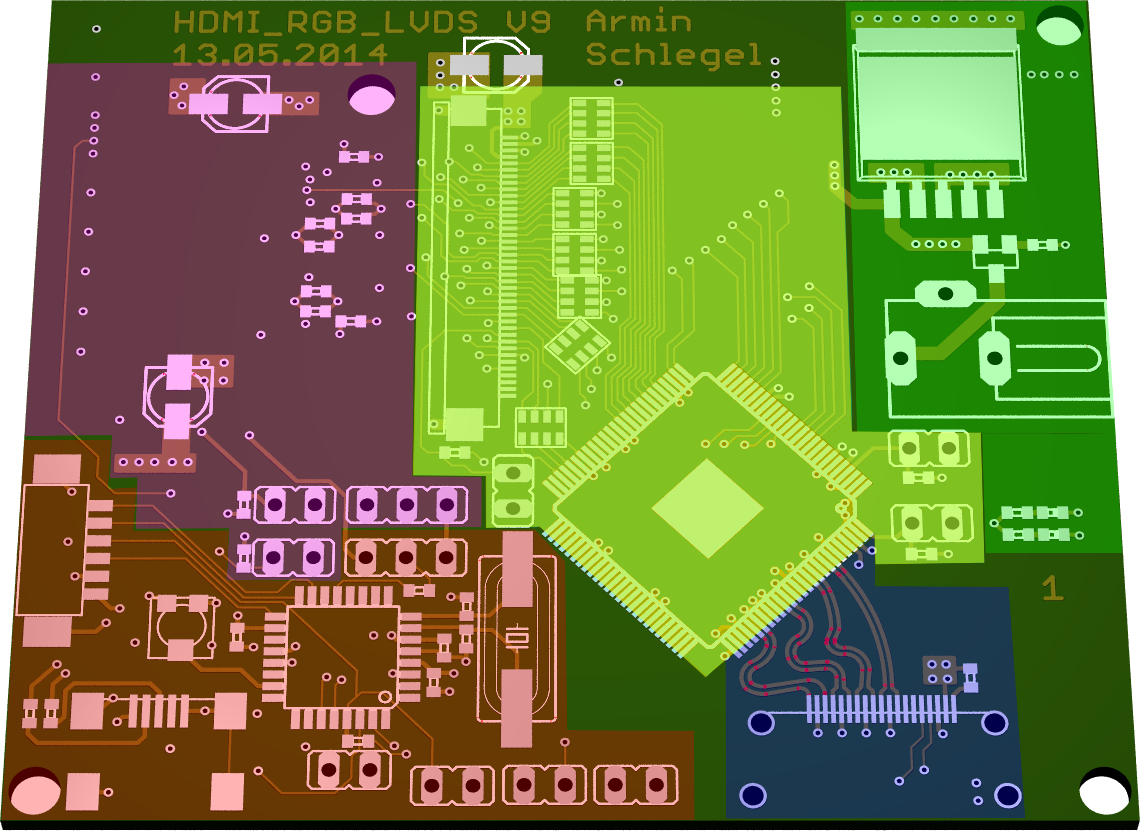
\includegraphics[height=4.7cm]{TeilB/HDMI_RGB_LVDS_V9_top.png}}
                \caption{Top Layer}
                \label{fig:teilb_pcb_top}
        \end{subfigure}
\quad 
        \begin{subfigure}[htp]{0.48\textwidth}
               \fbox{ 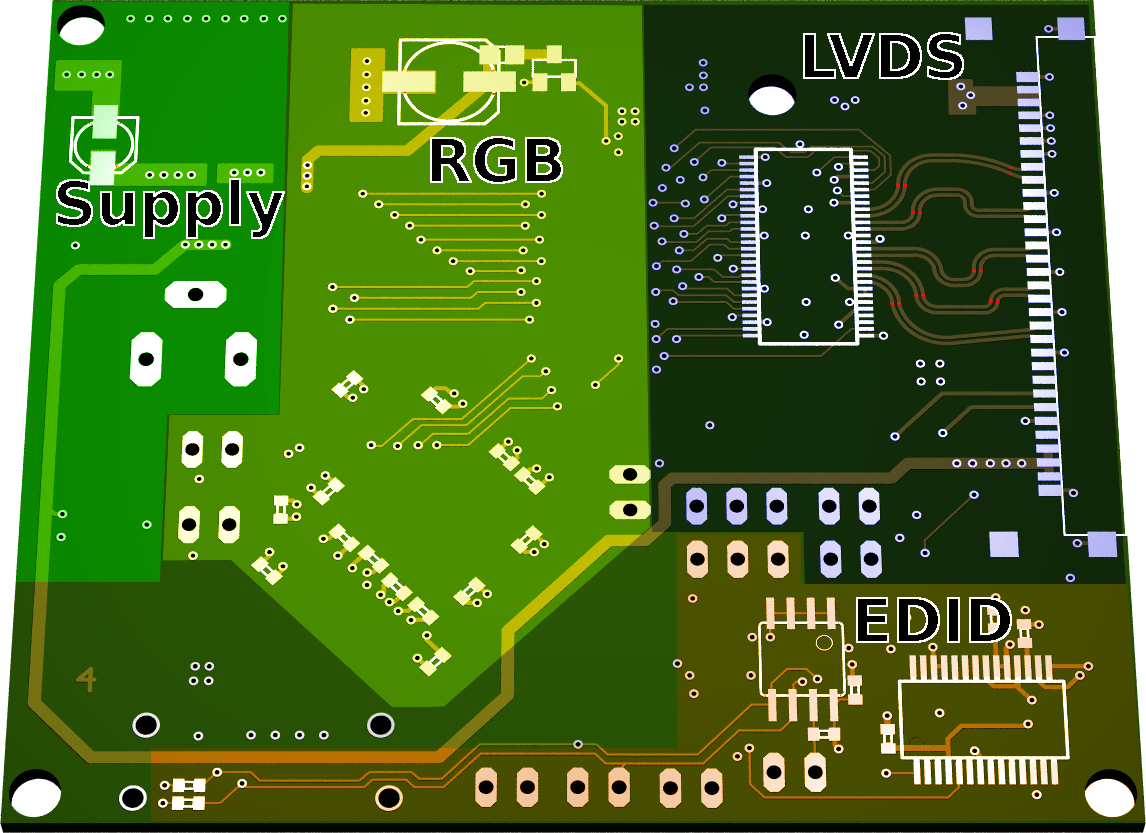
\includegraphics[height=4.7cm]{TeilB/HDMI_RGB_LVDS_V9_bot.png} }              				\caption{Bottom Layer}
                \label{fig:teilb_pcb_bot}
        \end{subfigure}
		%\end{center}
        \caption{HDMI RGB/LVDS Board}
        \label{fig:teilb_pcb}
\end{figure}

In den folgenden Abschnitten wird auf die Teilbereiche der Platine im Einzelnen eingegangen. Der Lagenaufbau ist entsprechend dem des Leiterplattenhersteller für vierlagige Platinen angelegt und ist in \refa{fig:teilb_lagenaufbau} zu sehen. Die Kupferdicke der einzelnen Lagen beträgt 35\,µm. Die beiden inneren Lagen sind als Versorgunglayer zur Leitung von Ground, +5\,V und +3.3\,V vorgesehen.
        \begin{figure}[htp]
        	\center
			\fbox{	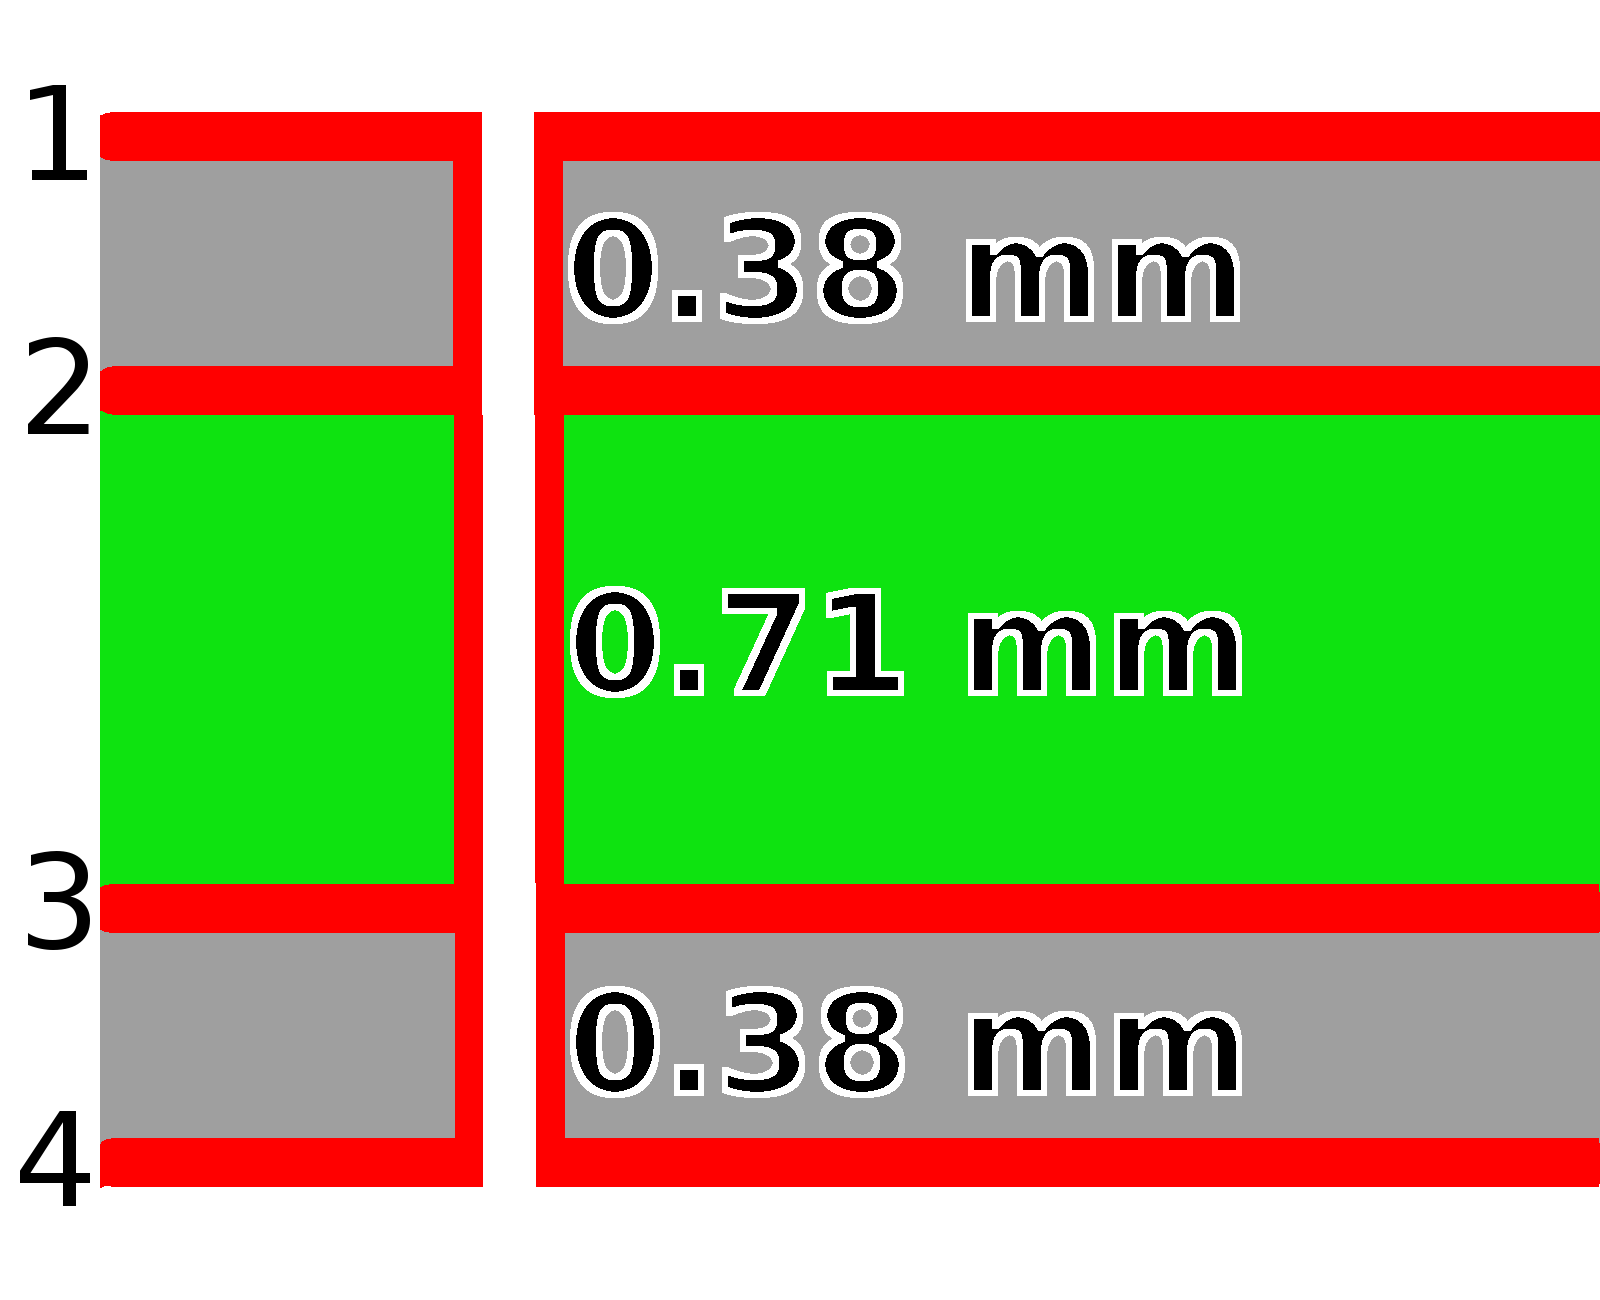
\includegraphics[width=0.3\textwidth]{TeilB/teilb_lagenaufbau.png}}
%			\fbox{	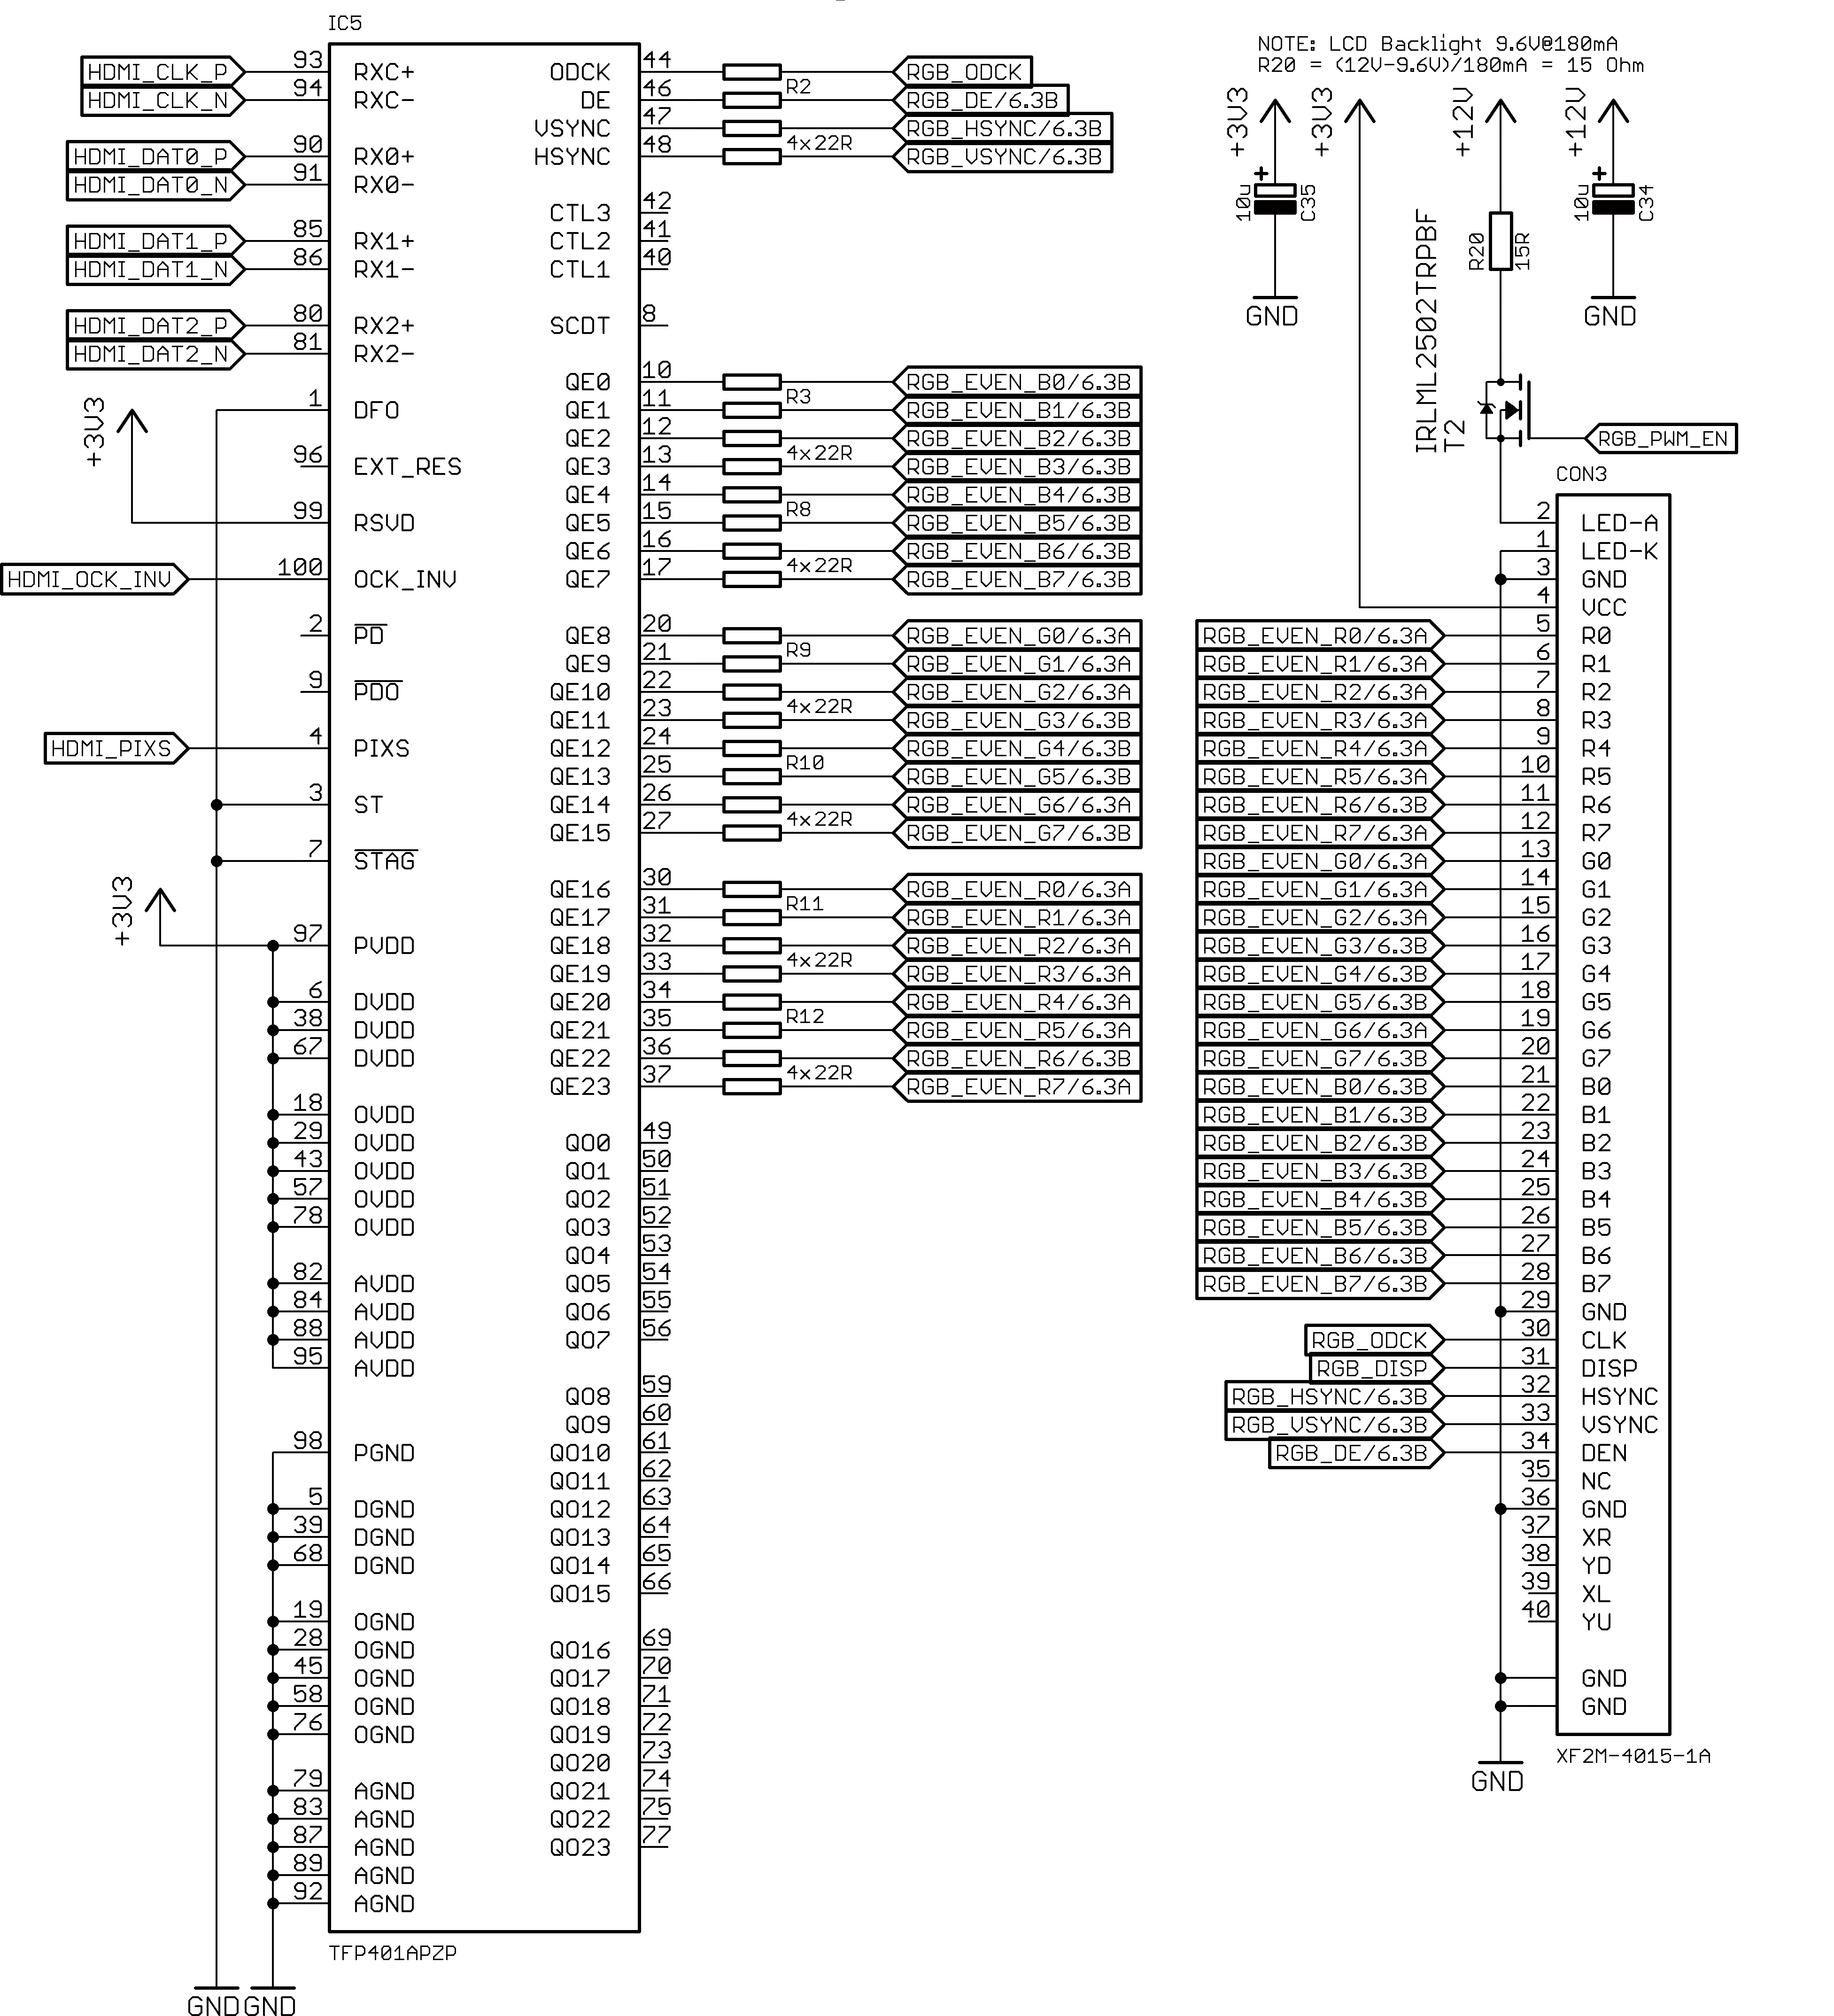
\includegraphics[width=8.5cm,keepaspectratio]{TeilB/rgb_bridge_sch.png}}
            \caption{Lagenaufbau Teil B}
            \label{fig:teilb_lagenaufbau}
        \end{figure}

\subsection{HDMI-Eingang}
\label{cha:hdmi_eingang}
Der HDMI-Eingang wird durch eine HDMI-Buchse der Firma \code{FCI} realisiert und wird mittels Impedanzkontrollierten Leitungen an die RGB-Bridge weitergegeben. Diese Leitungen sind mit einer differentielle Impedanz von 100\,$\Omega$ spezifiziert. Zu beachten ist, dass alle Leitungspaare dieselbe Länge aufweisen, da sonst Laufzeitunterschiede und Fehlabtastung innerhalb der verschiedenen Signalpaare auftreten und zu Fehlern führen können. Die Impedanz der differentieller Leitungen lässt sich nach den Gleichungen 
%
\begin{equation}
Z_0 = \frac{88.75}{\sqrt{\epsilon_r + 1.47}} \cdot ln\left(\frac{5.97 \cdot h}{0.8 \cdot W + t}\right)
\label{equ:z_0}
\end{equation}
%
und
%
\begin{equation}
Z_{Diff} = 2 \cdot Z_0  \cdot \left(1-0.48 \cdot e^{-0.96\frac{s}{h}}\right)
\label{equ:z_diff}
\end{equation}
%
mit den Parametern entsprechend \reft{tab:z_parameter} (siehe \cite{TI2007}) berechnen. Hier erhält man eine Impedanz $Z_0$ von 77\,$\Omega$ und eine differentielle Impedanz von 106\,$\Omega$. Aufgrund der kurzen Leitungslängen von maximal 11\,mm, spielt diese minimale Fehlanpassung keine große Rolle und kann vernachlässigt werden. Die Terminierung findet im Baustein statt und bedarf keiner externen Widerstände an den Enden der Leitungen.
\begin{table}[h]
\begin{tabular}{|p{7cm}|p{3cm}|p{3cm}|}\hline
\rowcolor{TableBackgroundColor} 
   \textbf{Parameter} & \textbf{Bezeichnung} & \textbf{Wert}	\\ \hline
    Dielektrikum 					& $\epsilon_r$	& 4.2		\\ \hline
	Breite der Leitungen  		 	& W 			& 0.28 mm	\\ \hline
	Abstand des Paares zueinander 	& s 			& 0.17 mm 	\\ \hline
	Dicke des Dielektrikums 		& h 			& 0.35 mm 	\\ \hline 
	Dicke der Leiterbahn 			& t 			& 35 µm		\\ \hline 
\end{tabular}
\caption{Parameter bezüglich Impedanz der HDMI-Leitungen}
\label{tab:z_parameter}
\end{table} \\
\refa{fig:teilb_hdmi} zeigt den Schaltplan und das Layout des HDMI-Steckeres. In \refa{fig:teilb_hdmi_pcb} sind die TMDS-Leitungspaare zu sehen, bei der ein gleichmäßiger Abstand zwischen den Leitungen einzelner Paare, sowie die gleiche Länge der Paare selbst eingehalten wird. 


\begin{figure}[htbp]
        %\begin{center}
        \centering
        \begin{subfigure}[htp]{0.48\textwidth}
%			\fbox{	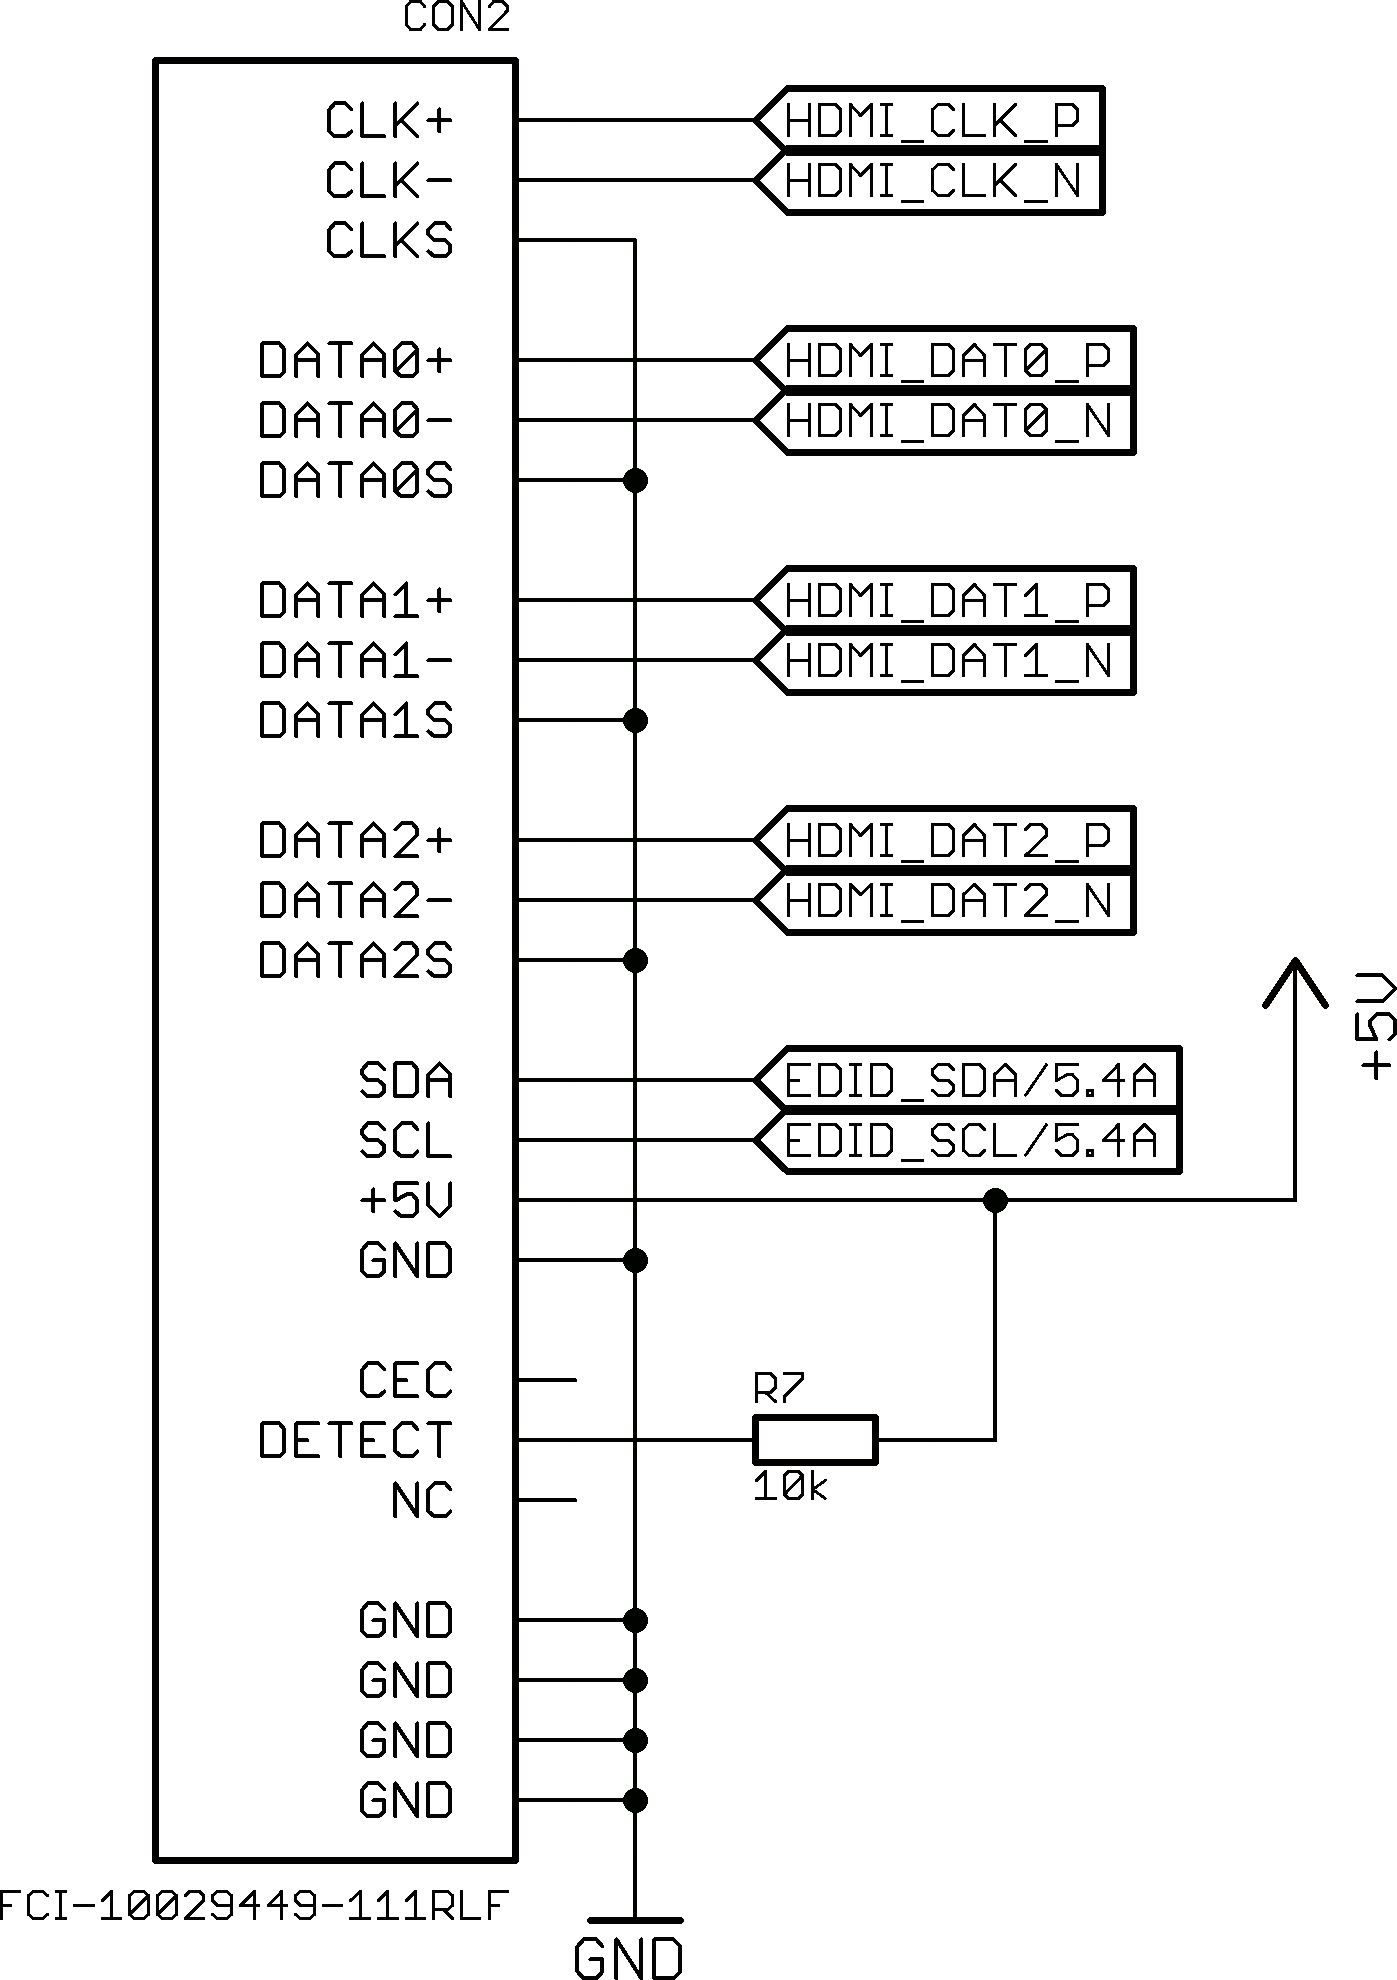
\includegraphics[width=1\textwidth]{TeilB/hdmi_sch.png}}
			\fbox{	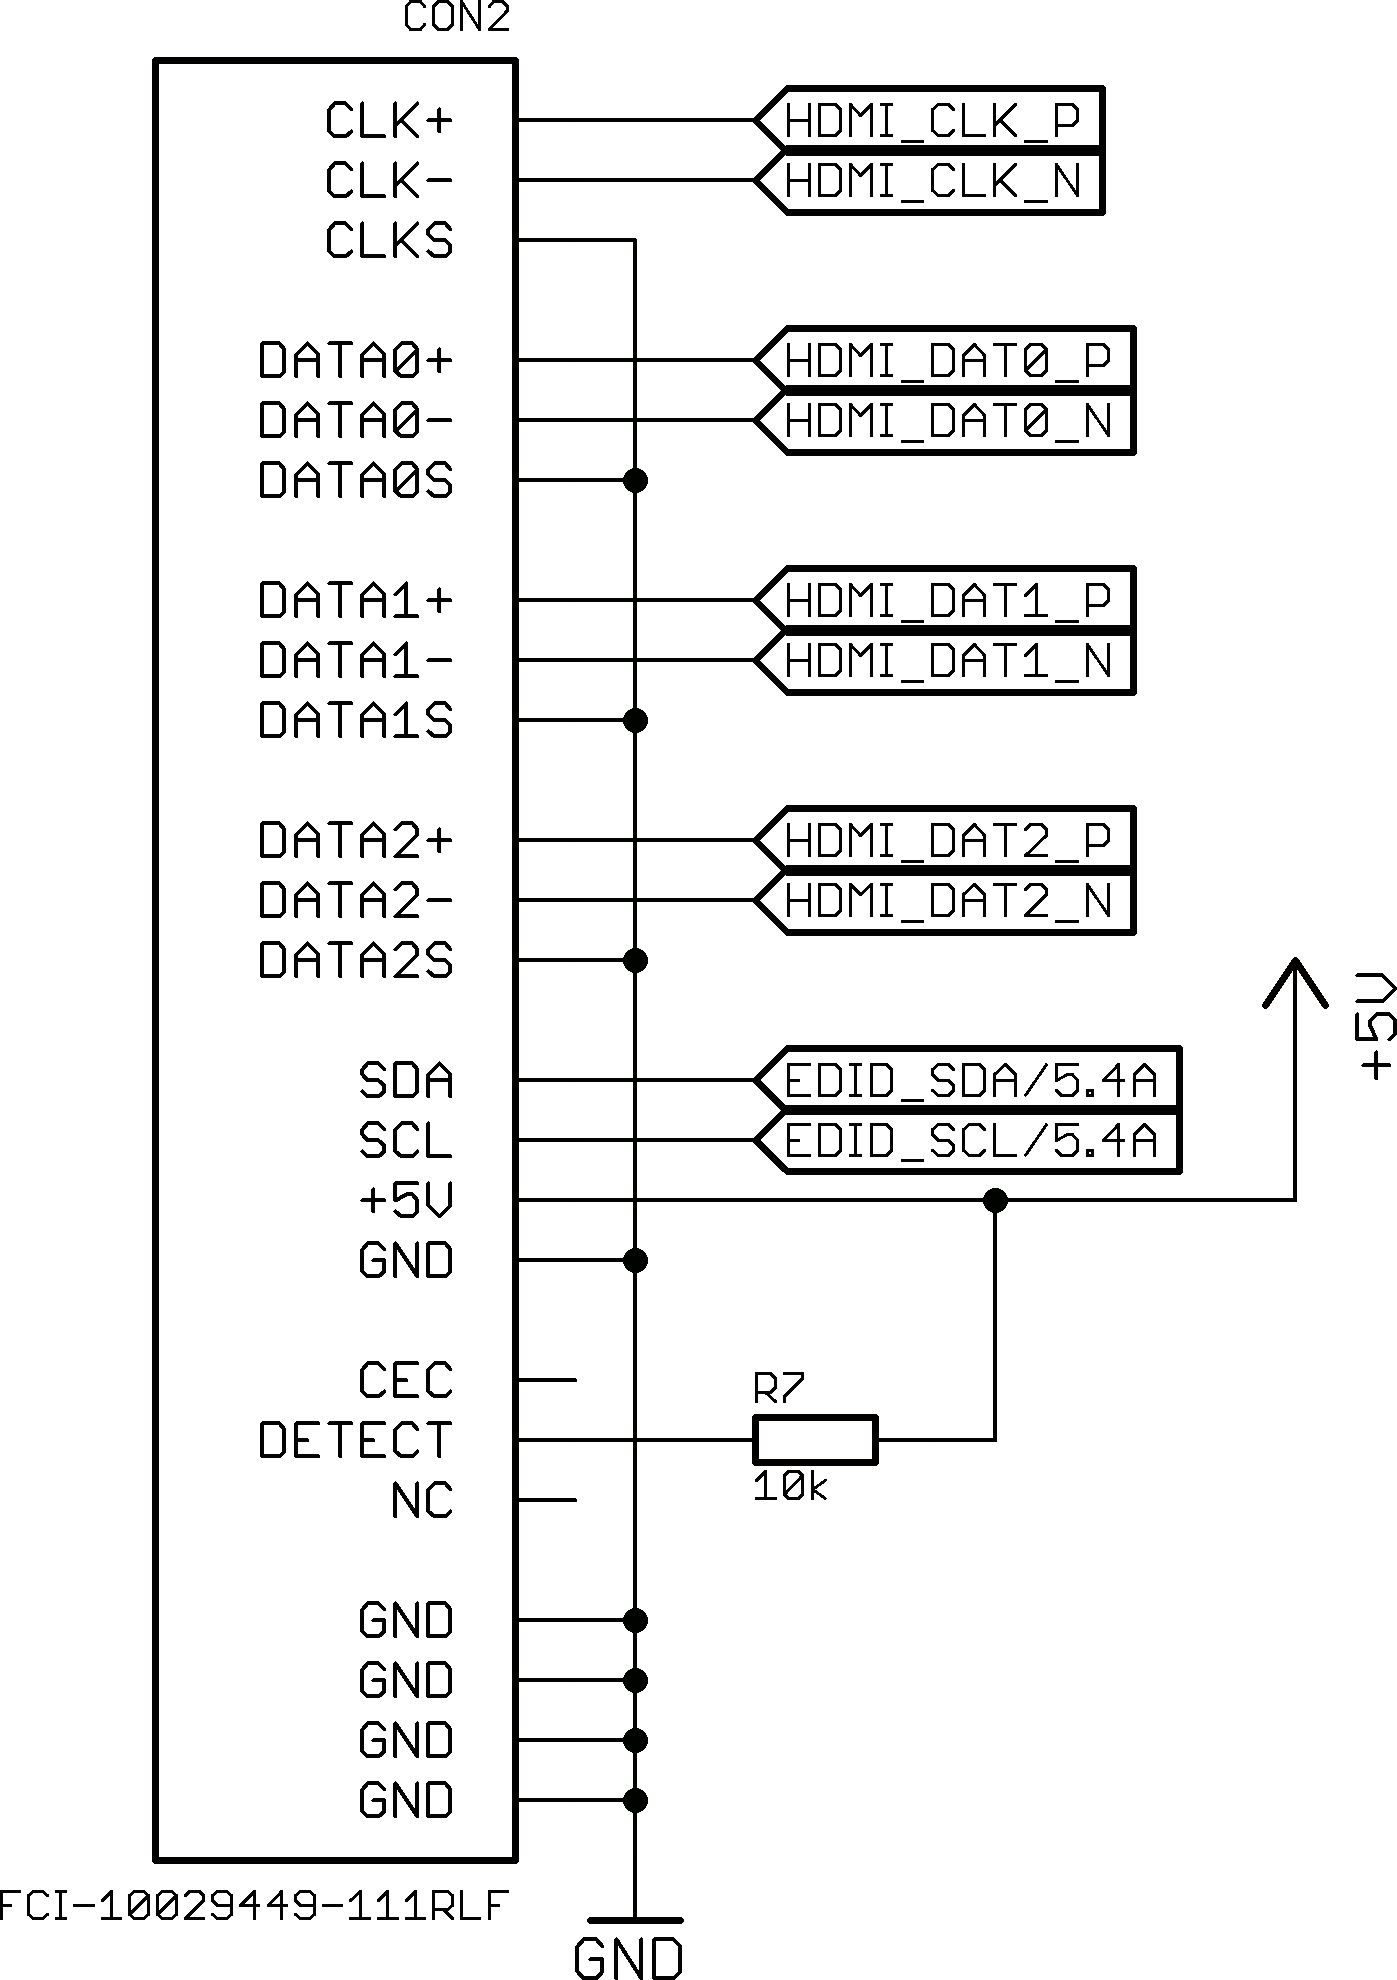
\includegraphics[height=6.5cm,width=1\textwidth,keepaspectratio]{TeilB/hdmi_sch.png}}
            \caption{HDMI-Stecker: Schaltplan}
            \label{fig:teilb_hdmi_sch}
        \end{subfigure}
\quad 
        \begin{subfigure}[htp]{0.48\textwidth}
			\fbox{	\includegraphics[height=6.5cm,width=1\textwidth,keepaspectratio]{TeilB/hdmi_stecker.png}}
 			\caption{HDMI Stecker: Layout}
            \label{fig:teilb_hdmi_pcb}
        \end{subfigure}
		%\end{center}
        \caption{HDMI Leitungen}
        \label{fig:teilb_hdmi}
\end{figure}
Neben den eigentlichen Video-Signalen befinden sich noch die $I^2C$-Signale \code{EDID_SCL}\footnote{EDID\_SCL: Taktleitung des $I^2C$-Bus} und \code{EDID_SDA}\footnote{EDID\_SDA: Datenleitung des $I^2C$-Bus} des EDID-EEPROMs sowie eine Hot-Plug-Detection auf der HDMI-Buchse.
\subsection{RGB-Bridge}
Die Eingänge der RGB-Bridge werden vom HDMI-Stecker gespeist. Die TMDS-Signale werden so aufbereitet, dass an den Ausgängen eine RGB-Schnittstelle zum Anschluss eines RGB-Panels bereitgestellt sind.
        \begin{figure}[htp]
        	\center
			\fbox{	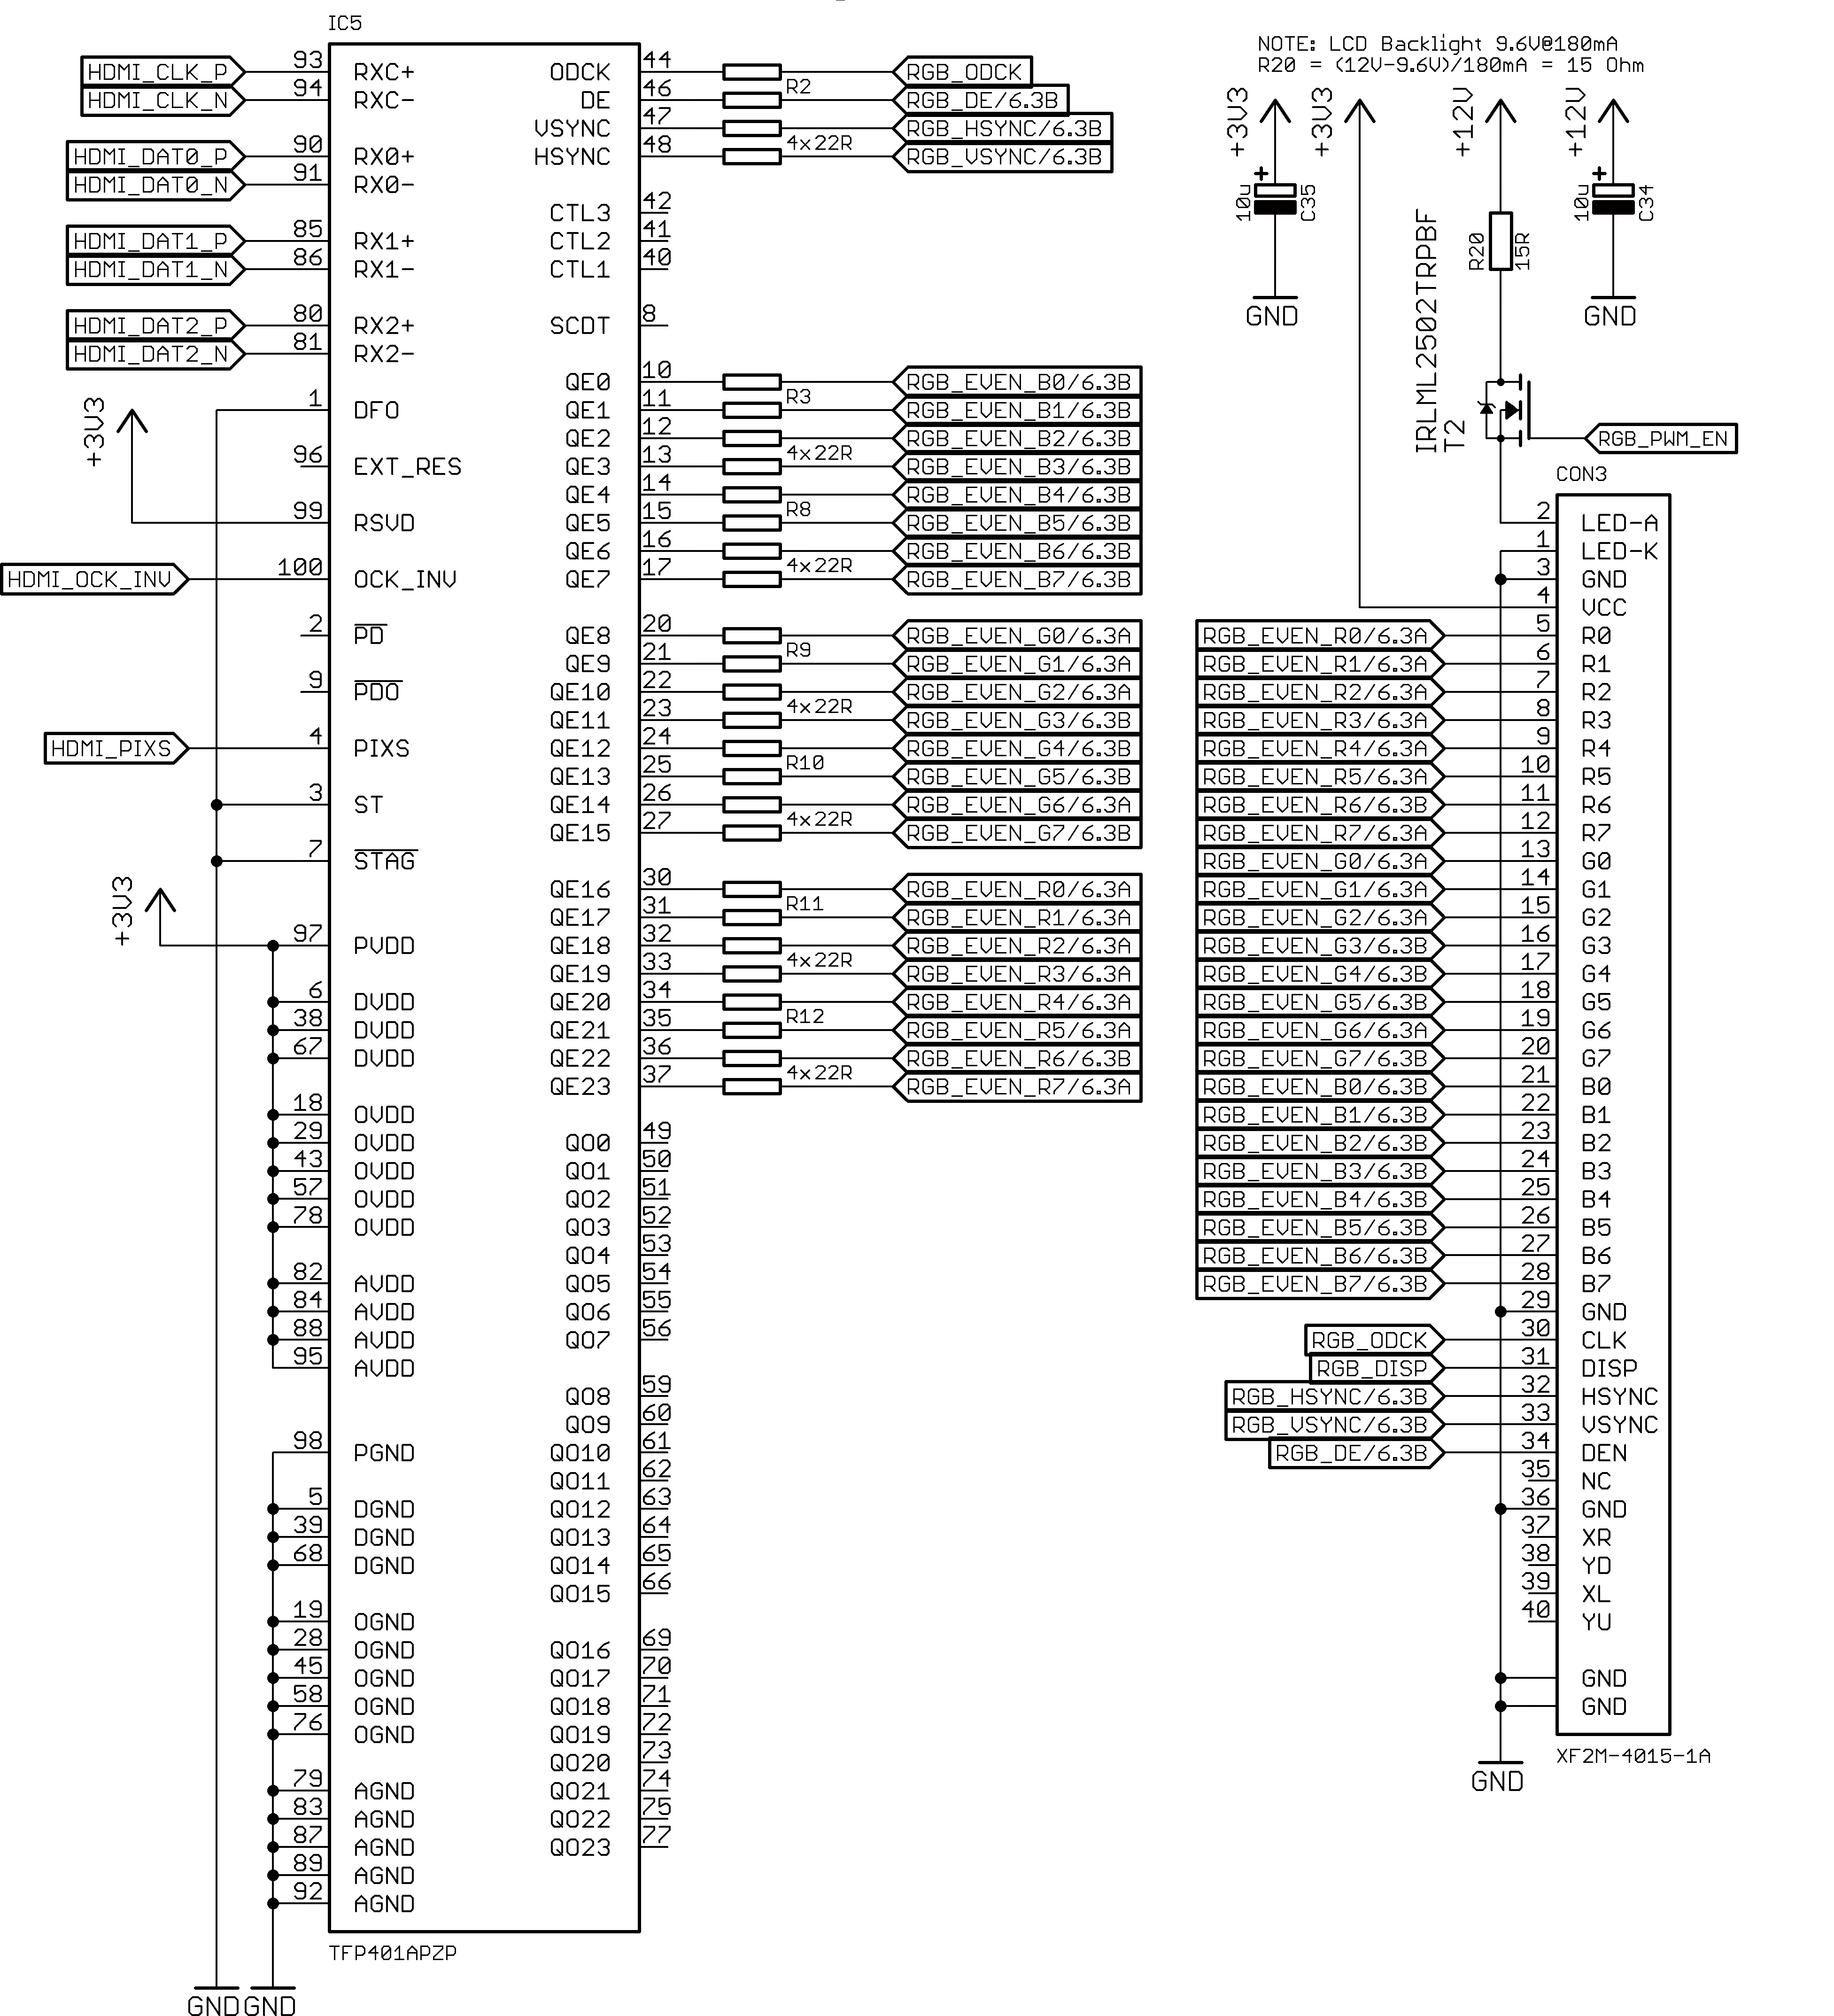
\includegraphics[width=0.9\textwidth]{TeilB/rgb_bridge_sch.png}}
%			\fbox{	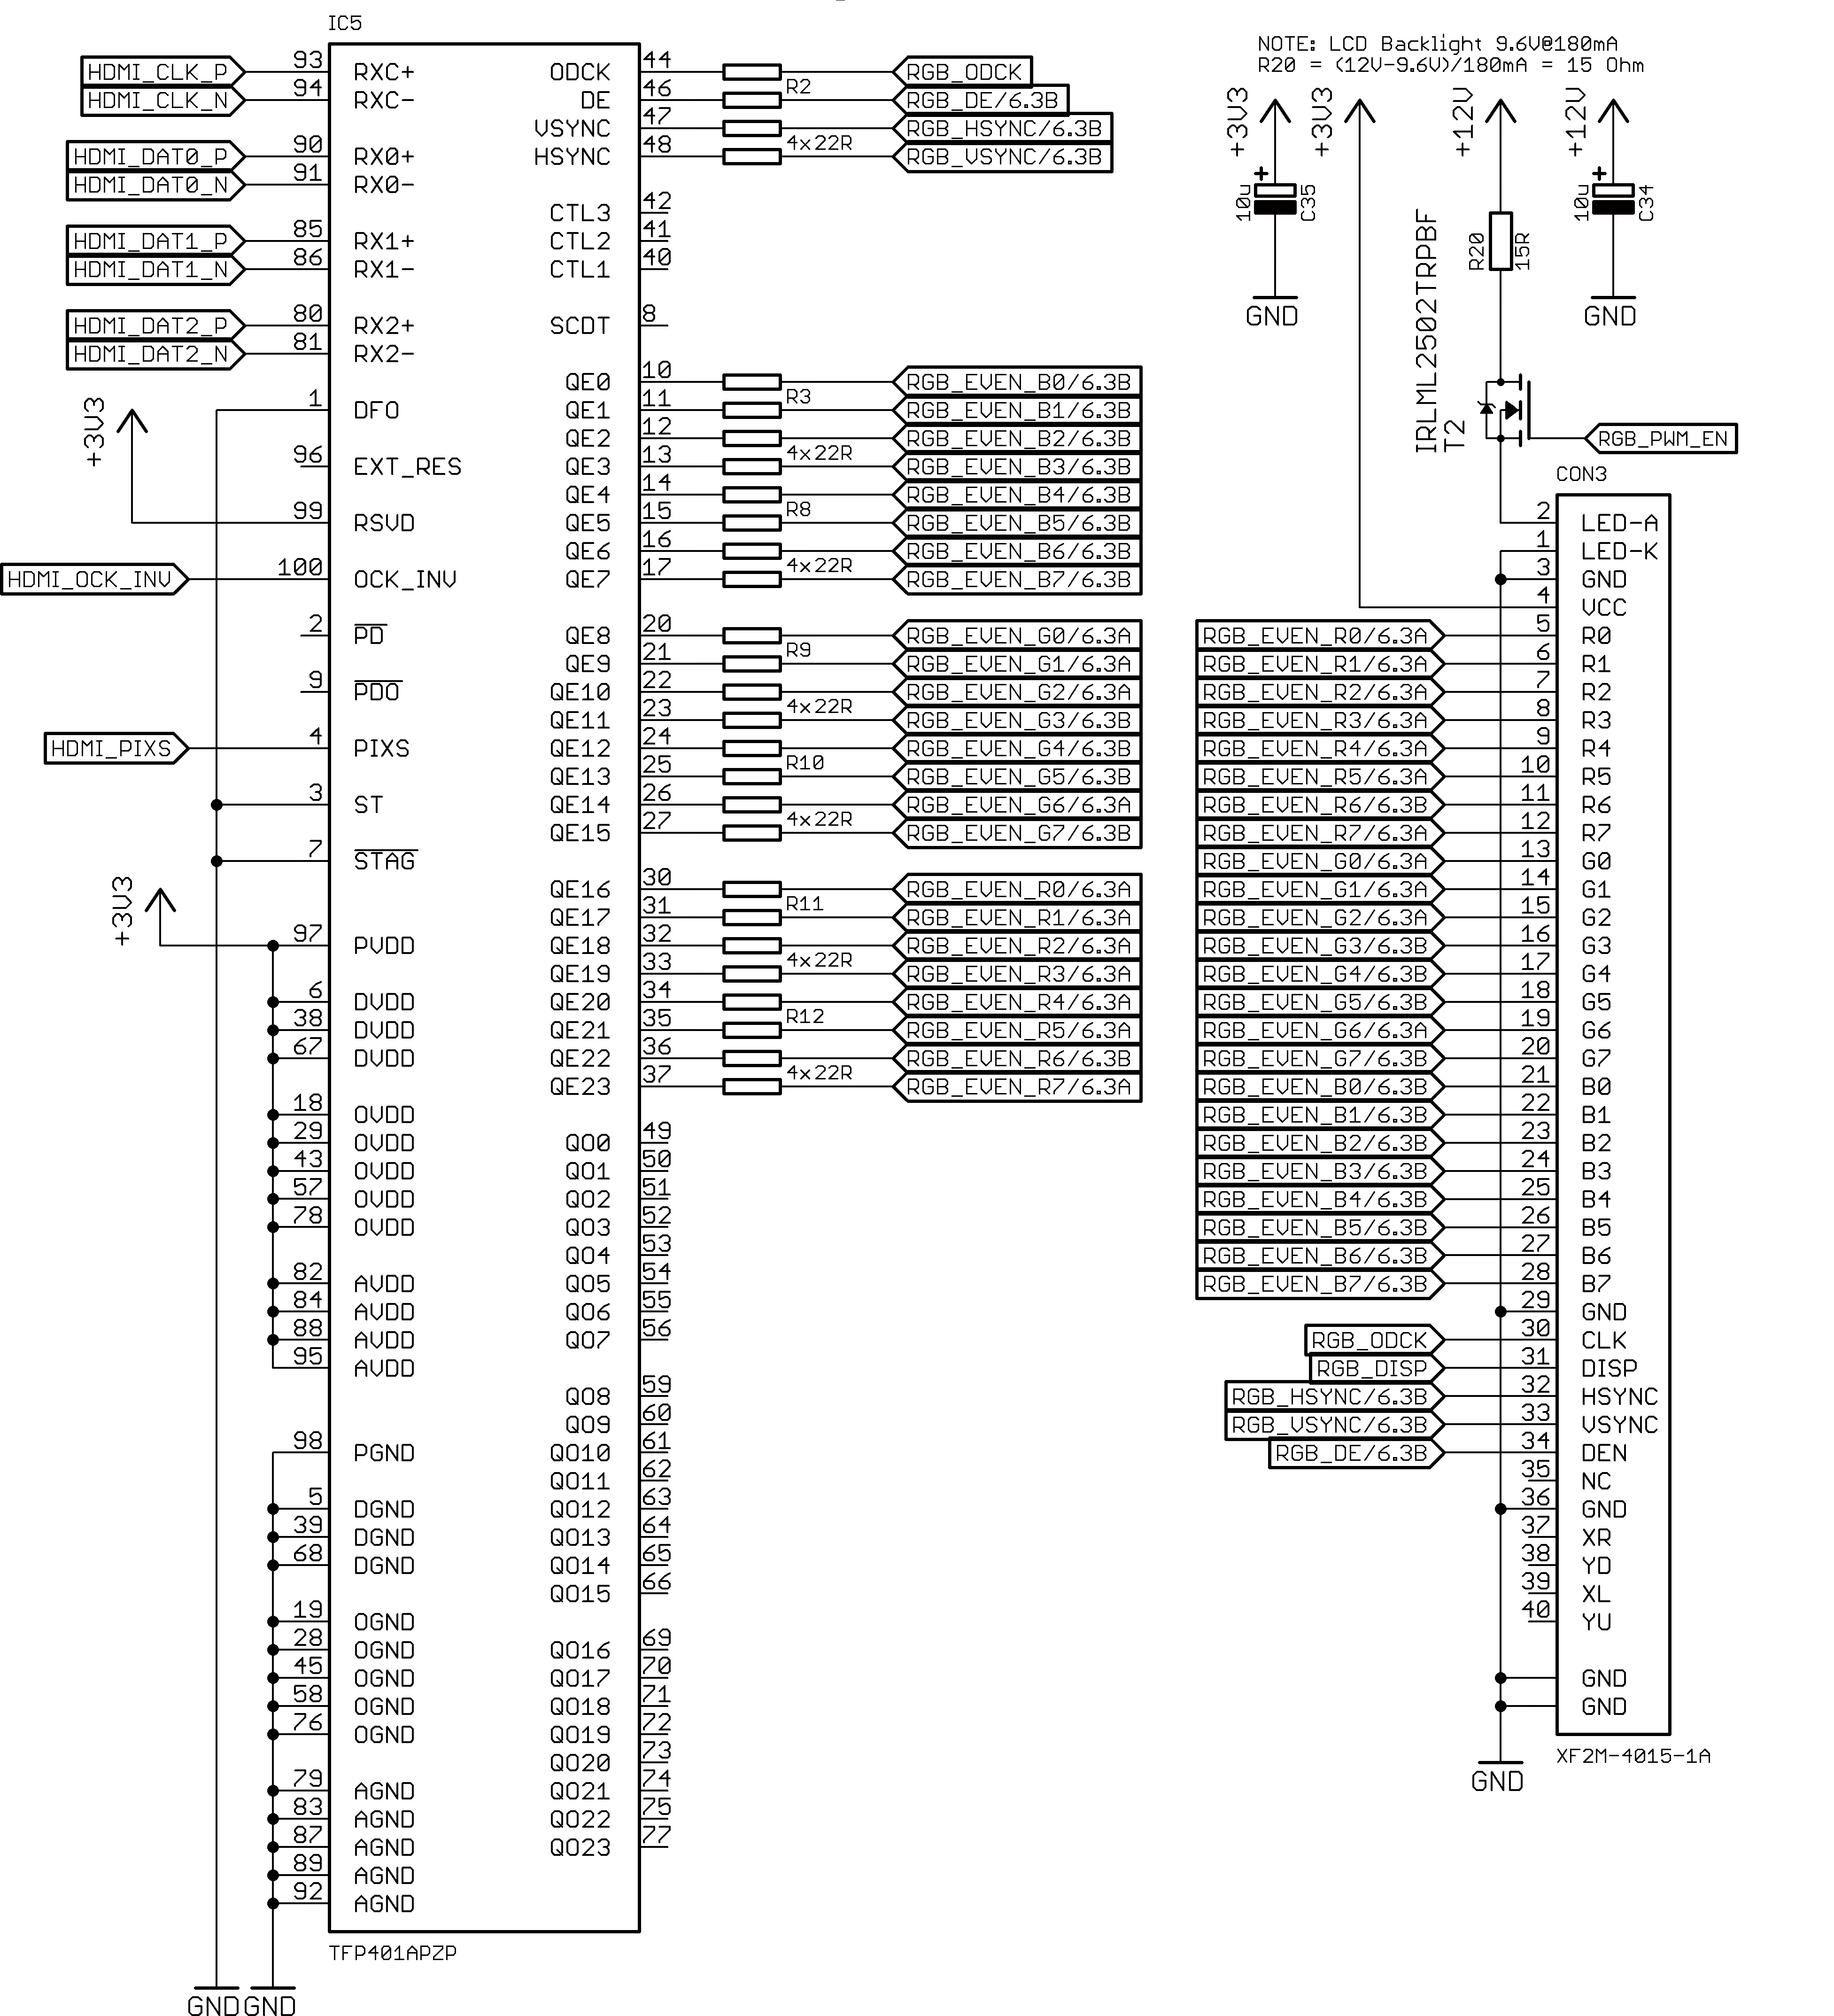
\includegraphics[width=8.5cm,keepaspectratio]{TeilB/rgb_bridge_sch.png}}
            \caption{RGB Bridge: Schaltplan}
            \label{fig:teilb_rgb_bridge_sch}
        \end{figure}
\newline        
\refa{fig:teilb_rgb_bridge_sch} zeigt den Schaltplan der RGB-Bridge mit dem Stecker für das RGB-Display. Als Baustein ist ein \code{TFP401A} von Texas Instruments im Einsatz. Neben den vier TMDS-Signalpaaren werden eingangsseitig noch die Signale \code{HDMI_PIXS} und \code{HDMI_OCK_INV} eingespeist. Diese sind zur Konfiguration der Ausgangssignale vorhanden. Ausgangsseitig sind die drei Farbkanäle für Rot, Grün und Blau (\code{RGB_EVEN_R[7:0]}, \code{RGB_EVEN_G[7:0]} und \code{RGB_EVEN_B[7:0]}) sowie die Steuersignale \code{RGB_ODCK}, \code{RGB_DE}, \code{RGB_HSYNC} und \code{RGB_VSYNC} verbunden.
Fließen Ströme mit hoher Frequenz, entstehen aufgrund des Induktionsgesetzes Störeffekte auf den Leitungen, die wiederum andere Signale beeinflussen können. Die induzierte Störspannung lässt sich mit der Gleichung
%
\begin{equation}
u \approx L \cdot \frac{di}{dt}
\label{equ:induzierte_spannung}
\end{equation}
%
berechnen. Steigt die Schaltfrequenz, und damit die Frequenz der Stromänderung $\frac{di}{dt}$, wird die abgestrahlte Störung ebenfalls stärker. Um diesem Effekt entgegenzuwirken, sind Serienwiderstände im Signalweg eingebaut, die mit der natürlichen Kapazität der Leitung den Tiefpasscharakter der Leitung besser ausprägt. Die Kapazität einer Mikrostreifenleitung lässt sich mit 
%
\begin{equation}
C_{Leiterbahn} = \epsilon_0 \cdot \epsilon_r \cdot \frac{(a+b) \cdot l}{d}
\label{equ:c_leiterbahn}
\end{equation}
%
für $\epsilon_0 = 8.86\cdot10^{-12} \frac{Am}{Vs}$, $\epsilon_r = 4.2$, der Leiterbahnbreite $a = 0.15 $mm, der Leiterbahndicke $b = 35$ µm, dem Abstand zur nächsten Fläche $d = 0.35$ mm und der durchschnittlichen Leiterbahnlänge $l = 50$ mm berechnen (siehe \cite{Gensicke2014}). Die durchschnittliche Kapazität der RGB-Leitungen beträgt somit rund 1\,pF. In Verbindung mit dem verwendeten 22\,$\Omega$ Widerstand bildet dieser in Verbindung mit der Leitung einen Tiefpass. Der quantitative Verlauf des Tiefpass deutet sich in \refa{fig:teilb_tiefpass_mess} an, wobei Grün die originale und Blau die gefilterte Kurve darstellt. Zu erkennen ist, dass die Steilheit der fallenden und steigenden Flanke abnimmt, was zu einer verlangsamten Stromänderung $\frac{di}{dt}$ führt.
\begin{figure}[htbp]
			\fbox{	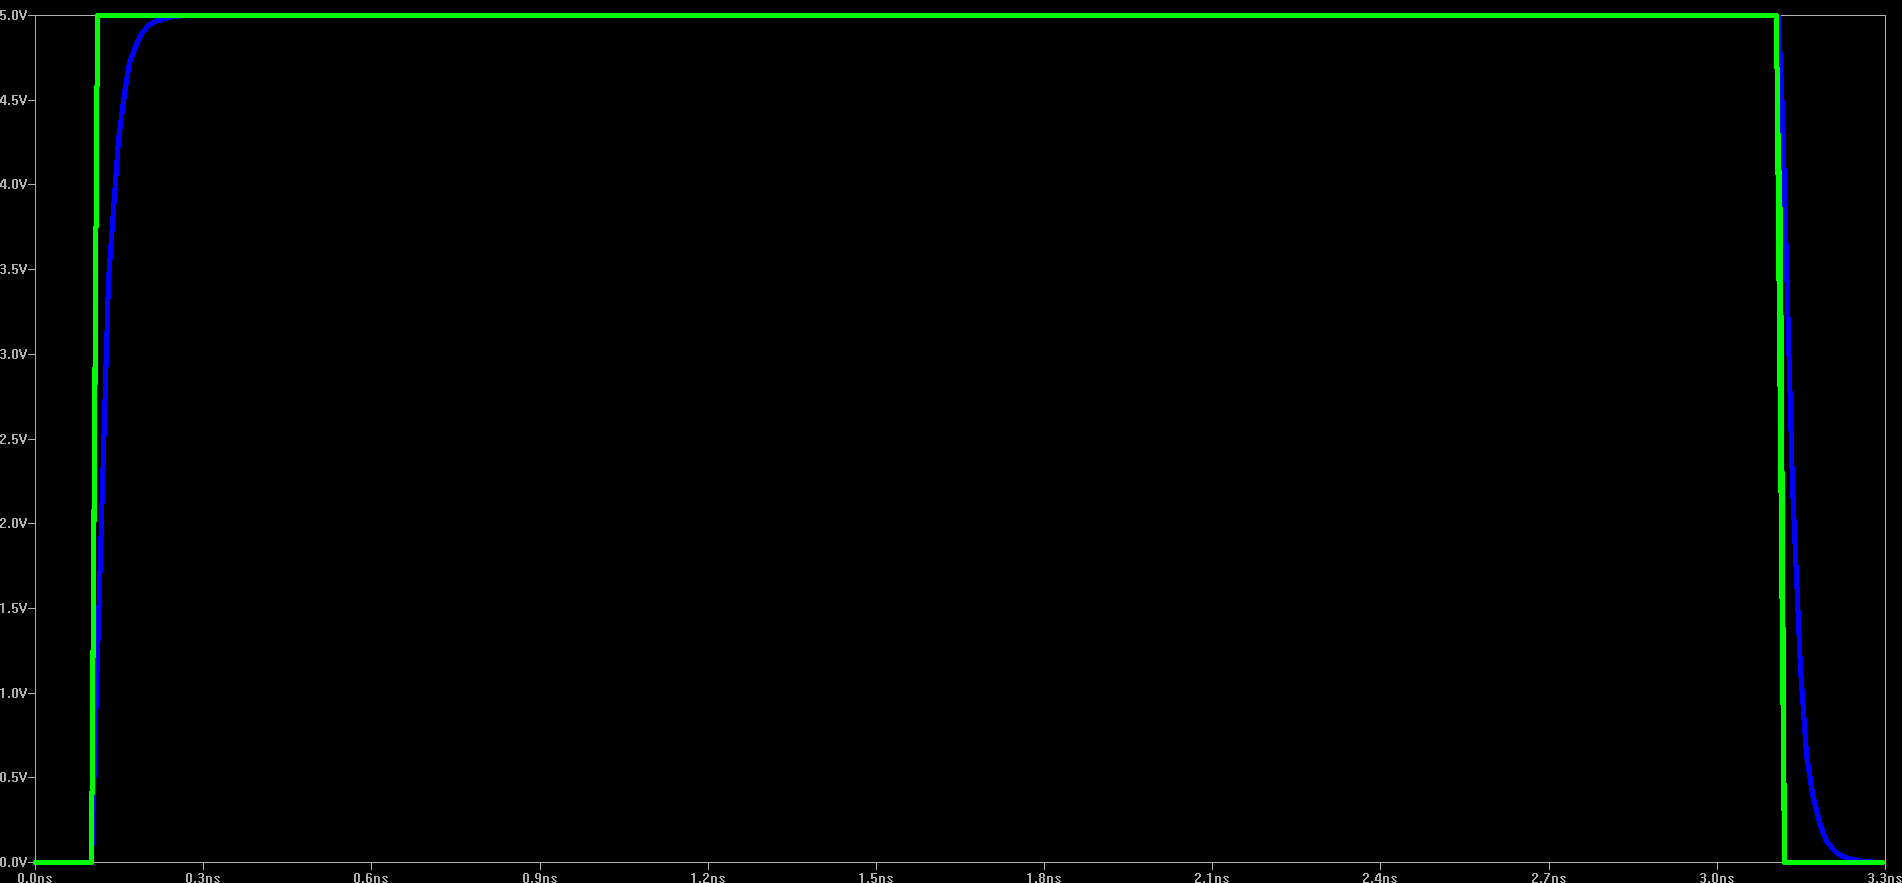
\includegraphics[width=1\textwidth,keepaspectratio]{TeilB/sim_serienwiderstand_messung.png}}
 			\caption{RGB Bridge: Simulationsergebnis des Leitungstiefpass}
            \label{fig:teilb_tiefpass_mess}
\end{figure}
Das Layout der RGB-Signale, gezeigt in \refa{fig:teilb_rgb_bridge_pcb}, ist unkritischer als das der HDMI-Signale, da beim verwendeten Display ein maximaler Pixeltakt von 33\,MHz auftritt (siehe \cite{LG2012}, S.14). Aufgrund der noch relativ langsamen Taktung, haben eventuell auftretende Laufzeitunterschiede zwischen den Signale einen vernachlässigbaren Effekt. Die Serienwiderstände sind als Widerstands-Array mit je vier realisiert.
\begin{figure}[htp]
	\center
	\fbox{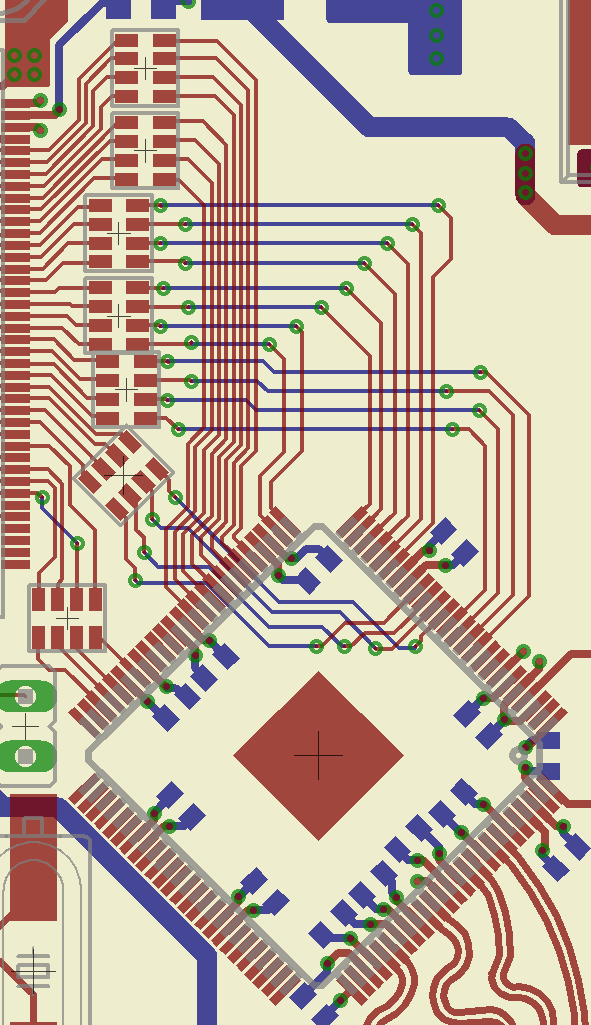
\includegraphics[height=0.8\textwidth,keepaspectratio,angle=90]{TeilB/rgb_bridge_pcb.png}}
 	\caption{RGB Bridge: Layout, gedreht um 90$^{\circ}$} 
    \label{fig:teilb_rgb_bridge_pcb}
\end{figure}
\newpage
\subsection{LVDS-Bridge}
Die LVDS-Bridge teilt die am Eingang liegenden parallelen RGB-Signale in Pakete zu je acht Bit auf und übertragt diese seriell über die verfügbaren LVDS-Kanäle. Die Beschaltung der LVDS-Bridge ist daher auf das verwendete Display \code{LB070WV8-SL01} zugeschnitten und analog den Abbildungen \ref{fig:teilb_lvds_bridge_format} und \ref{fig:teilb_lvds_display_format} zu verbinden.
\begin{figure}[htbp]
        %\begin{center}
        \begin{center}
        \begin{subfigure}[htp]{0.48\textwidth}
			\fbox{	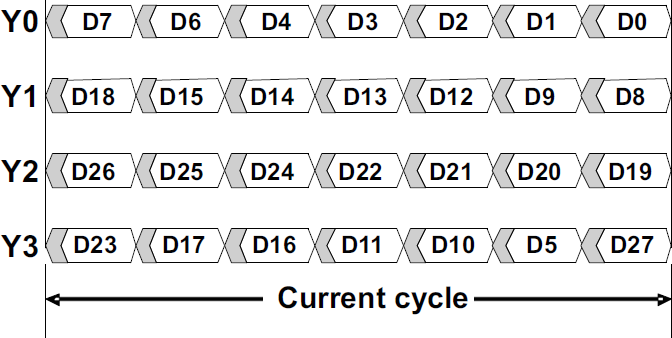
\includegraphics[height=3.3cm]{TeilB/lvds_bridge_paket.png}}
 			\caption{Paketformat LVDS-Bridge, \cite{TI2011b}}
            \label{fig:teilb_lvds_bridge_format}
        \end{subfigure}
        \quad
        \begin{subfigure}[htp]{0.48\textwidth}
			\fbox{	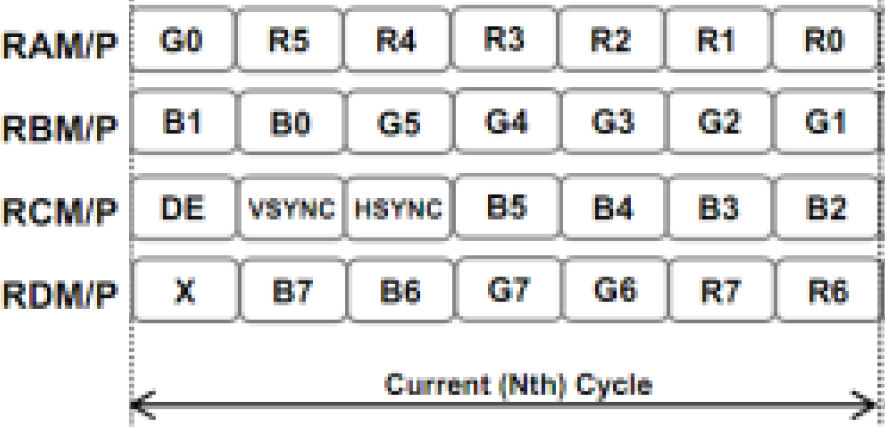
\includegraphics[height=3.3cm]{TeilB/lvds_display_paket.png}}
            \caption{Paketformat LVDS-Display, \cite{LG2012}}
            \label{fig:teilb_lvds_display_format}
        \end{subfigure}
		\end{center}
        \caption{LVDS Paketformate}
        \label{fig:teilb_lvds_format}
\end{figure} \\
So liegt zum Beispiel das RGB Bit G4 auf dem Dateneingang D13 der LVDS-Bridge. Der Schaltplan in \refa{fig:teilb_lvds_bridge_sch} zeigt die Beschaltung der LVDS-Bridge und des Steckverbinders für das Display.\\
\begin{figure}[htp]
		\center
		\fbox{	\includegraphics[width=0.8\textwidth]{TeilB/lvds_bridge_sch.png}}
%			\fbox{	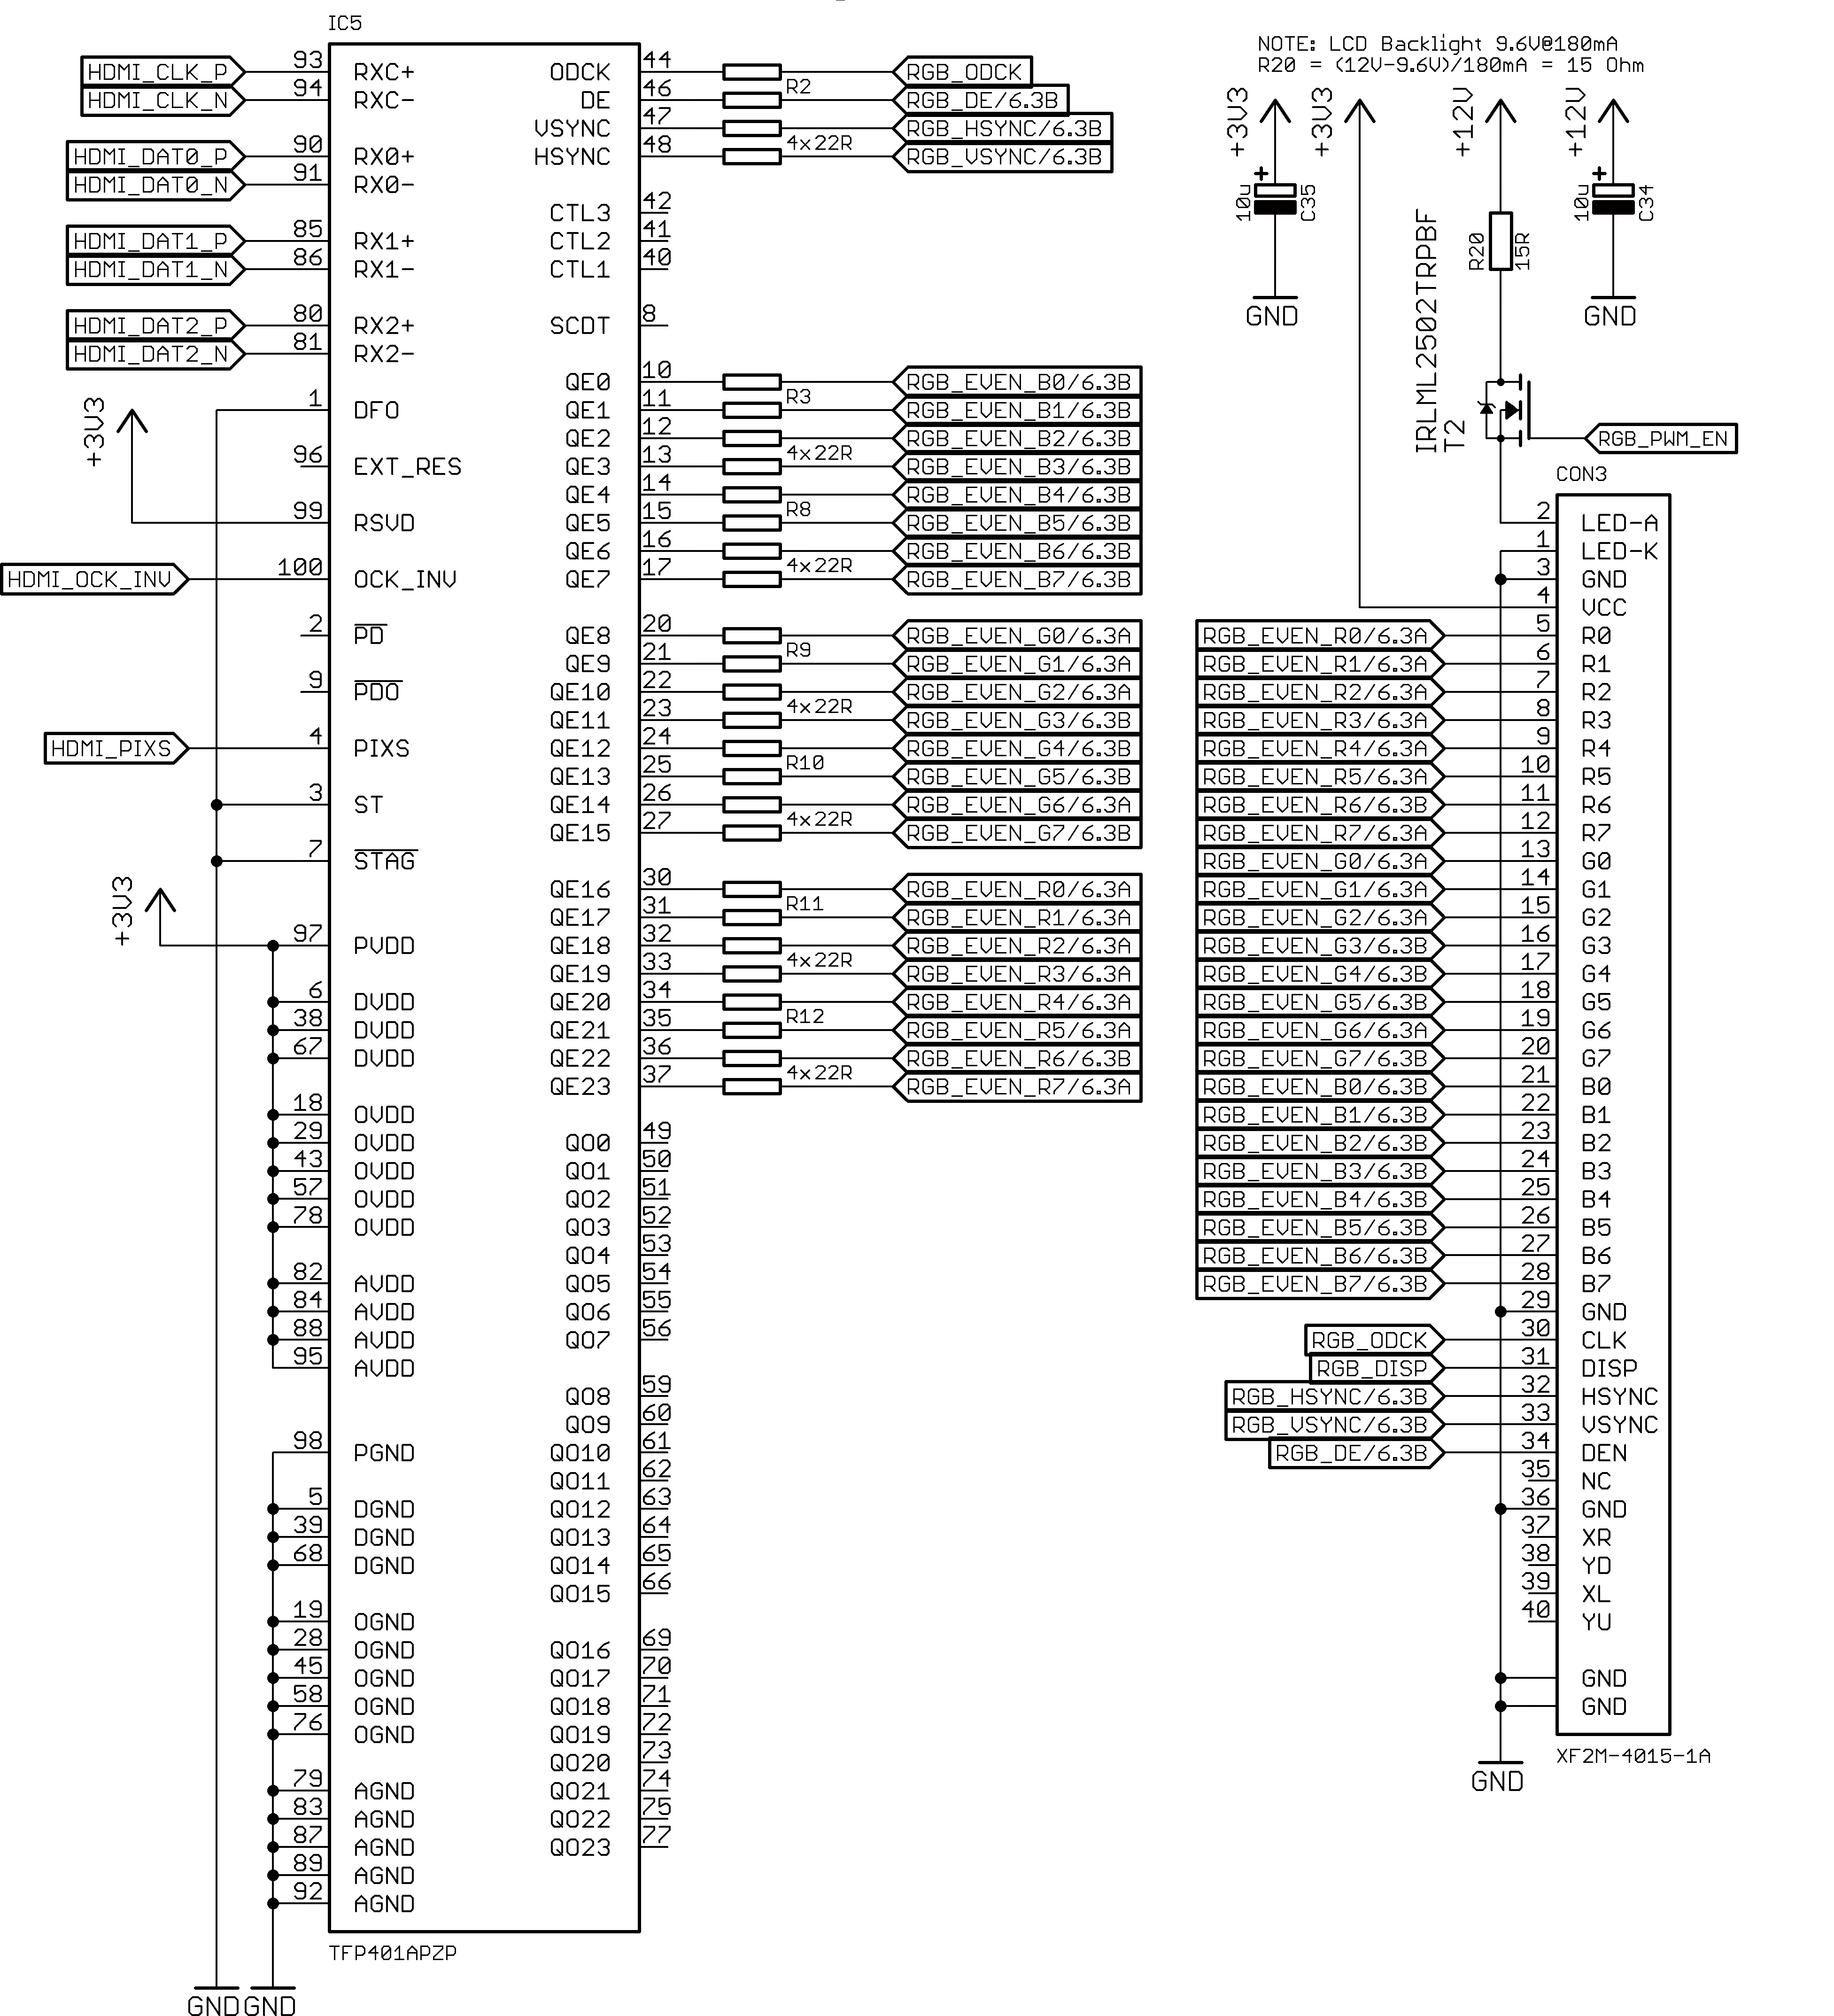
\includegraphics[width=8.5cm,keepaspectratio]{TeilB/rgb_bridge_sch.png}}
        \caption{LVDS Bridge: Schaltplan}
       \label{fig:teilb_lvds_bridge_sch}
\end{figure}\\
Wie auch bei den HDMI-Leitungen muss beim Layouten ein besonderes Augenmerk geworfen werden. Da hier ebenfalls eine Impedanz von 100\,$\Omega$ gefordert werden, sind dieselben Parameter bzgl. Leitungsbreite und Abstand wie in Abschnitt \ref{cha:hdmi_eingang} verwendet, bei der sich eine differentielle Impedanz von 106\,$\Omega$ errechnet.  Die Terminierung findet am Ende der LVDS-Leitungen im Display statt und bedarf keiner zusätzlichen Bauteile auf der Platine. Wie zuvor ist die Länge der Leitungspaare zueinander enorm wichtig. Die Längen der Leitungspaare sind im Bereich zwischen 13.825\,mm und 14.010\,mm, was einer maximalen Abweichung von 1.34 \% entspricht. Durch die angepasste differentielle Impedanz und gleichlangen Leitungen, ist die LVDS-Strecke hinreichend gut dimensioniert. \refa{fig:teilb_lvds_bridge_pcb} zeigt das Layout der LVDS-Bridge. Um die RGB-Signale vom Top-Layer auf den Bottom-Layer zu bekommen, werden diese mit Vias\footnote{Via: Durchkontaktierung} verbunden. Um große Umwege für Rückströme zu verhindern, ist zwischen den Durchkontaktierungen ausreichend Platz, sodass die Vias vollständig von einer Ground-Fläche umschlossen werden.
\begin{figure}[htp]
		\center
		\fbox{	\includegraphics[width=0.6\textwidth,angle=90]{TeilB/lvds_bridge_pcb.png}}
%			\fbox{	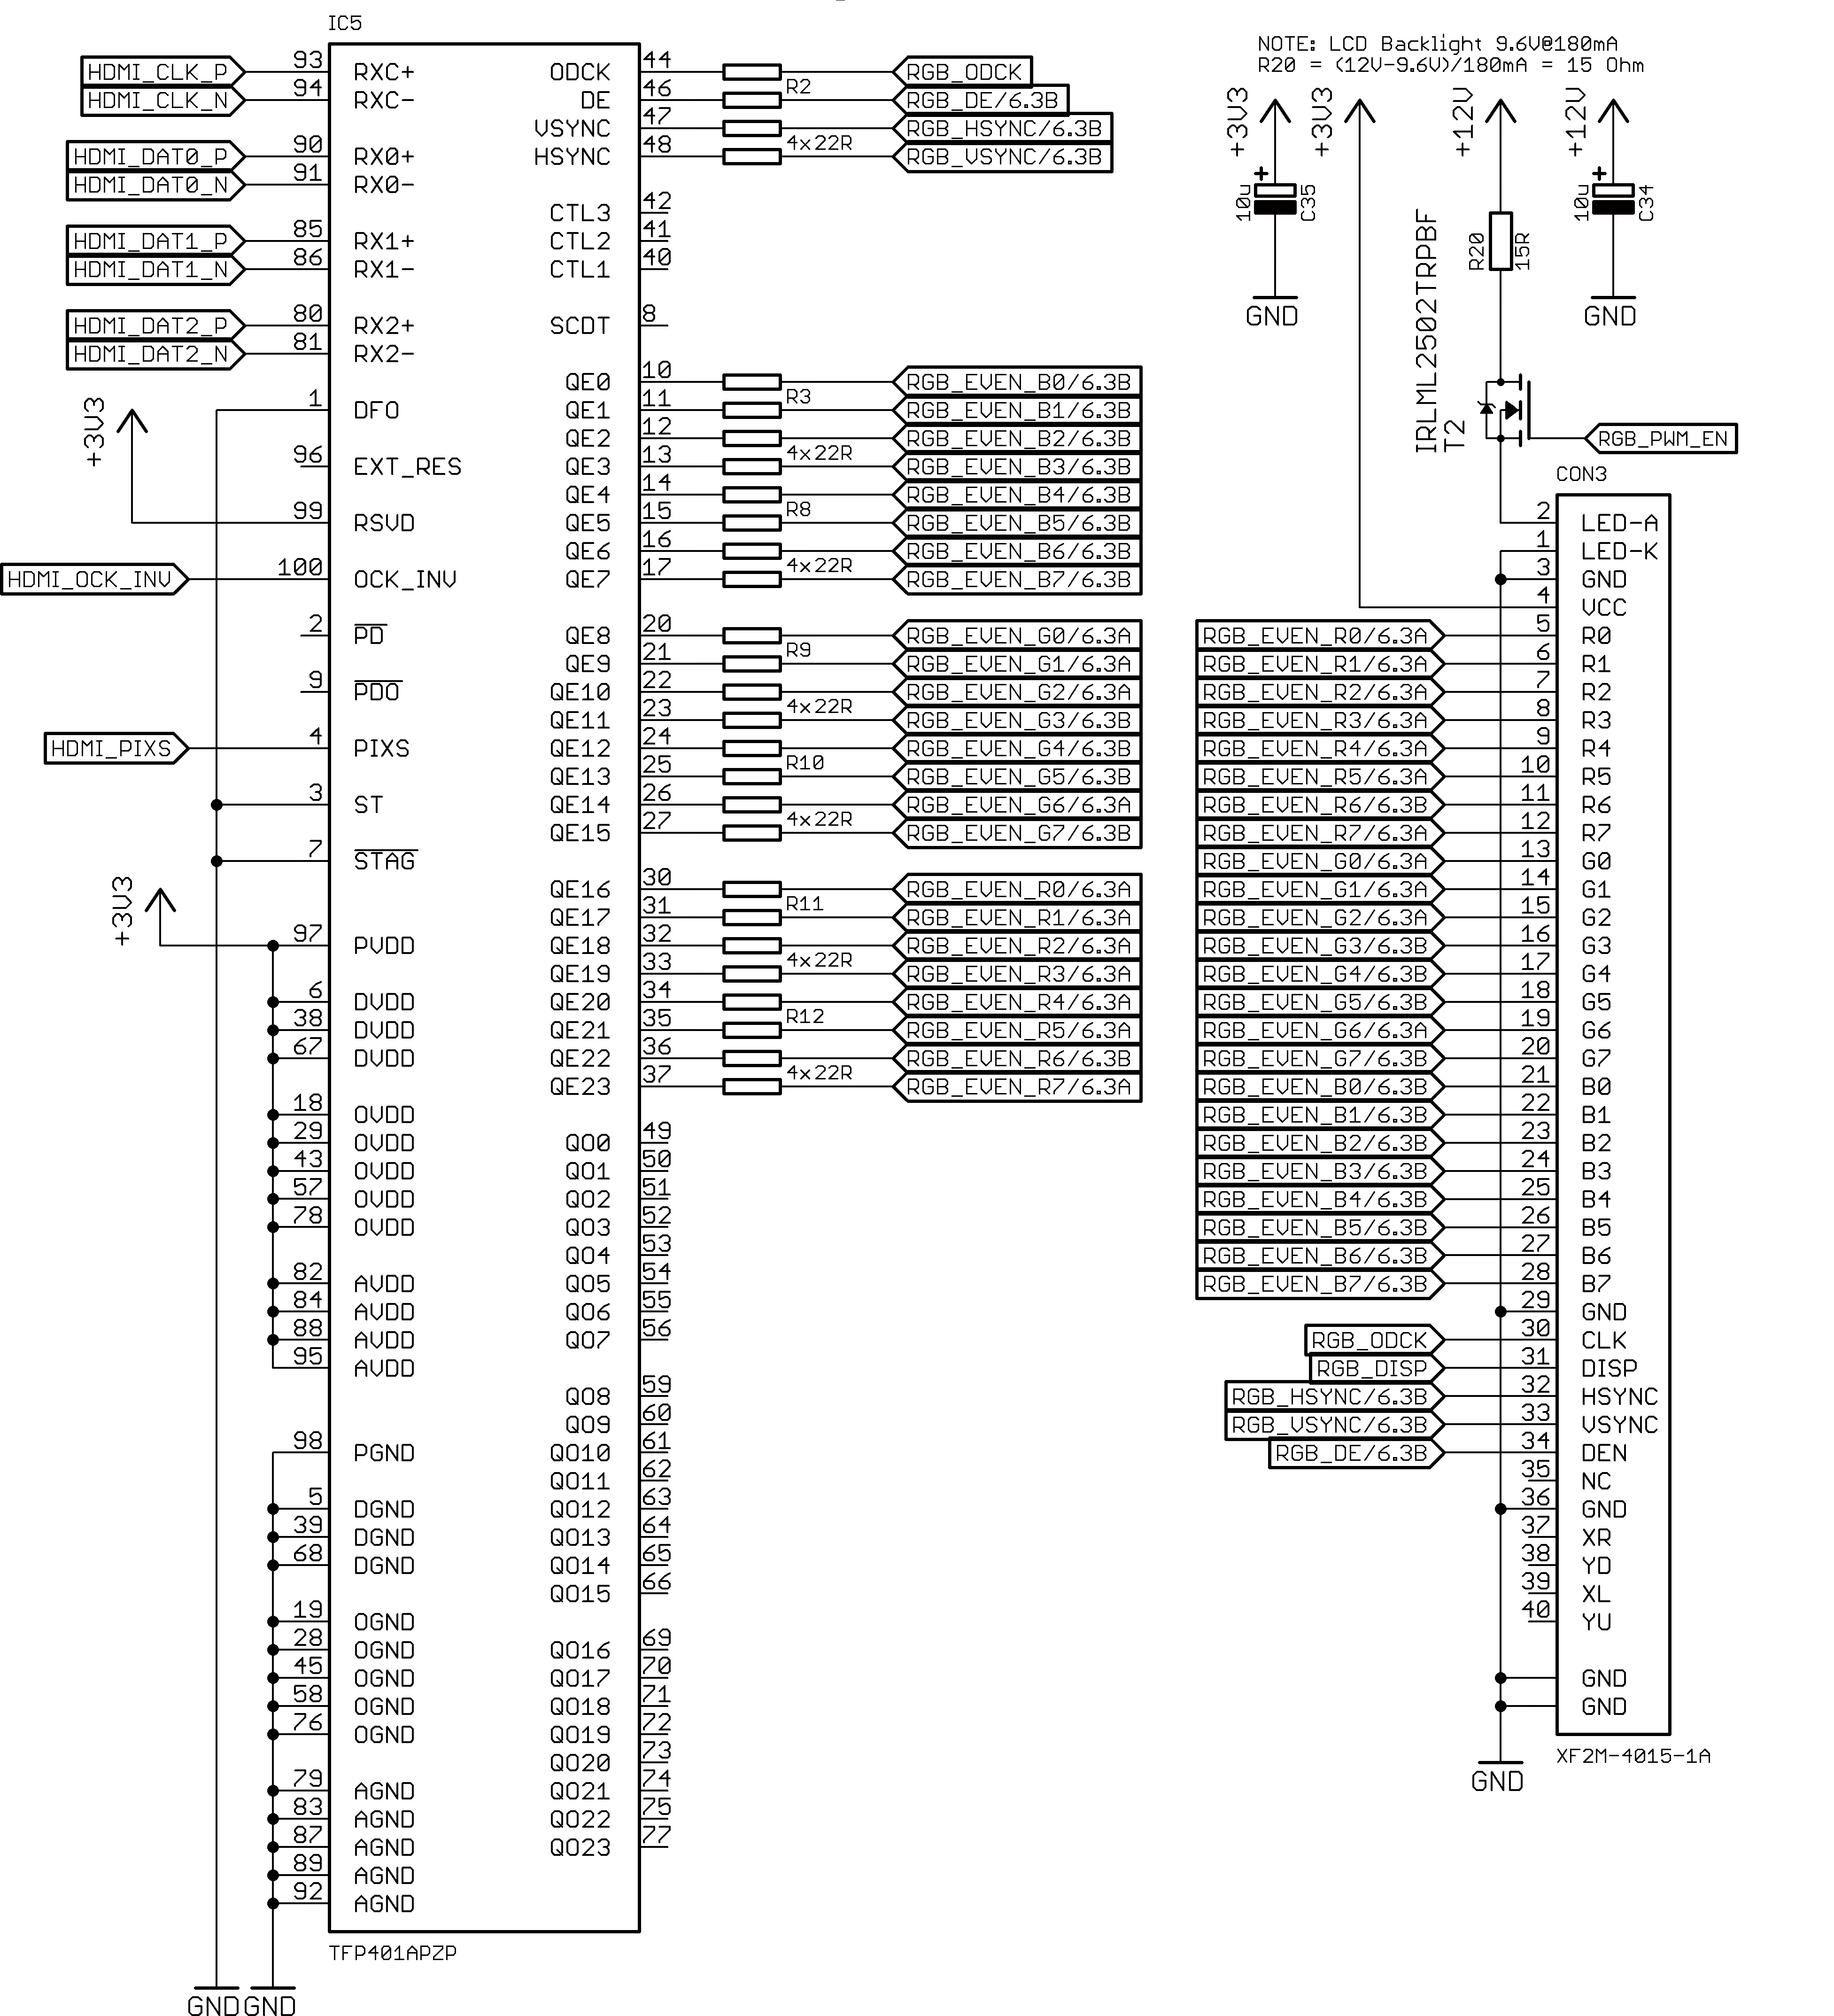
\includegraphics[width=8.5cm,keepaspectratio]{TeilB/rgb_bridge_sch.png}}
        \caption{LVDS Bridge: Layout, gedreht um 90$^{\circ}$}
       \label{fig:teilb_lvds_bridge_pcb}
\end{figure}
\newpage
\subsection{EDID-Daten}
\label{cha:sw_edid_daten}
Wie bereits in \refc{sec:TeilB_Konzept} angesprochen ist ein EEPROM vorhanden, welches die EDID-Informationen beinhaltet. Ohne diese Informationen ist ein Plug-And-Play-Betrieb der Hardware an einer HDMI-Quelle nicht möglich, da der Quelle nicht mitgeteilt wird, welche Randbedingungen an Timings und Auflösung das Anzeigegerät benötigt. Um den Anschluss von verschiedenen RGB- oder LVDS-Displays zu gewährleisten, können die EDID-Daten über eine integrierte USB-Buchse und dem zugehörigen Programm direkt auf der Hardware programmiert werden. \refa{fig:teilb_edid_blockschaltbild} zeigt einen Ausschnitt aus \refa{fig:teilb_architektur}, das die einzelnen Komponenten des EDID-Blocks darstellt. 
\begin{figure}[htp]
	\center
	\fbox{	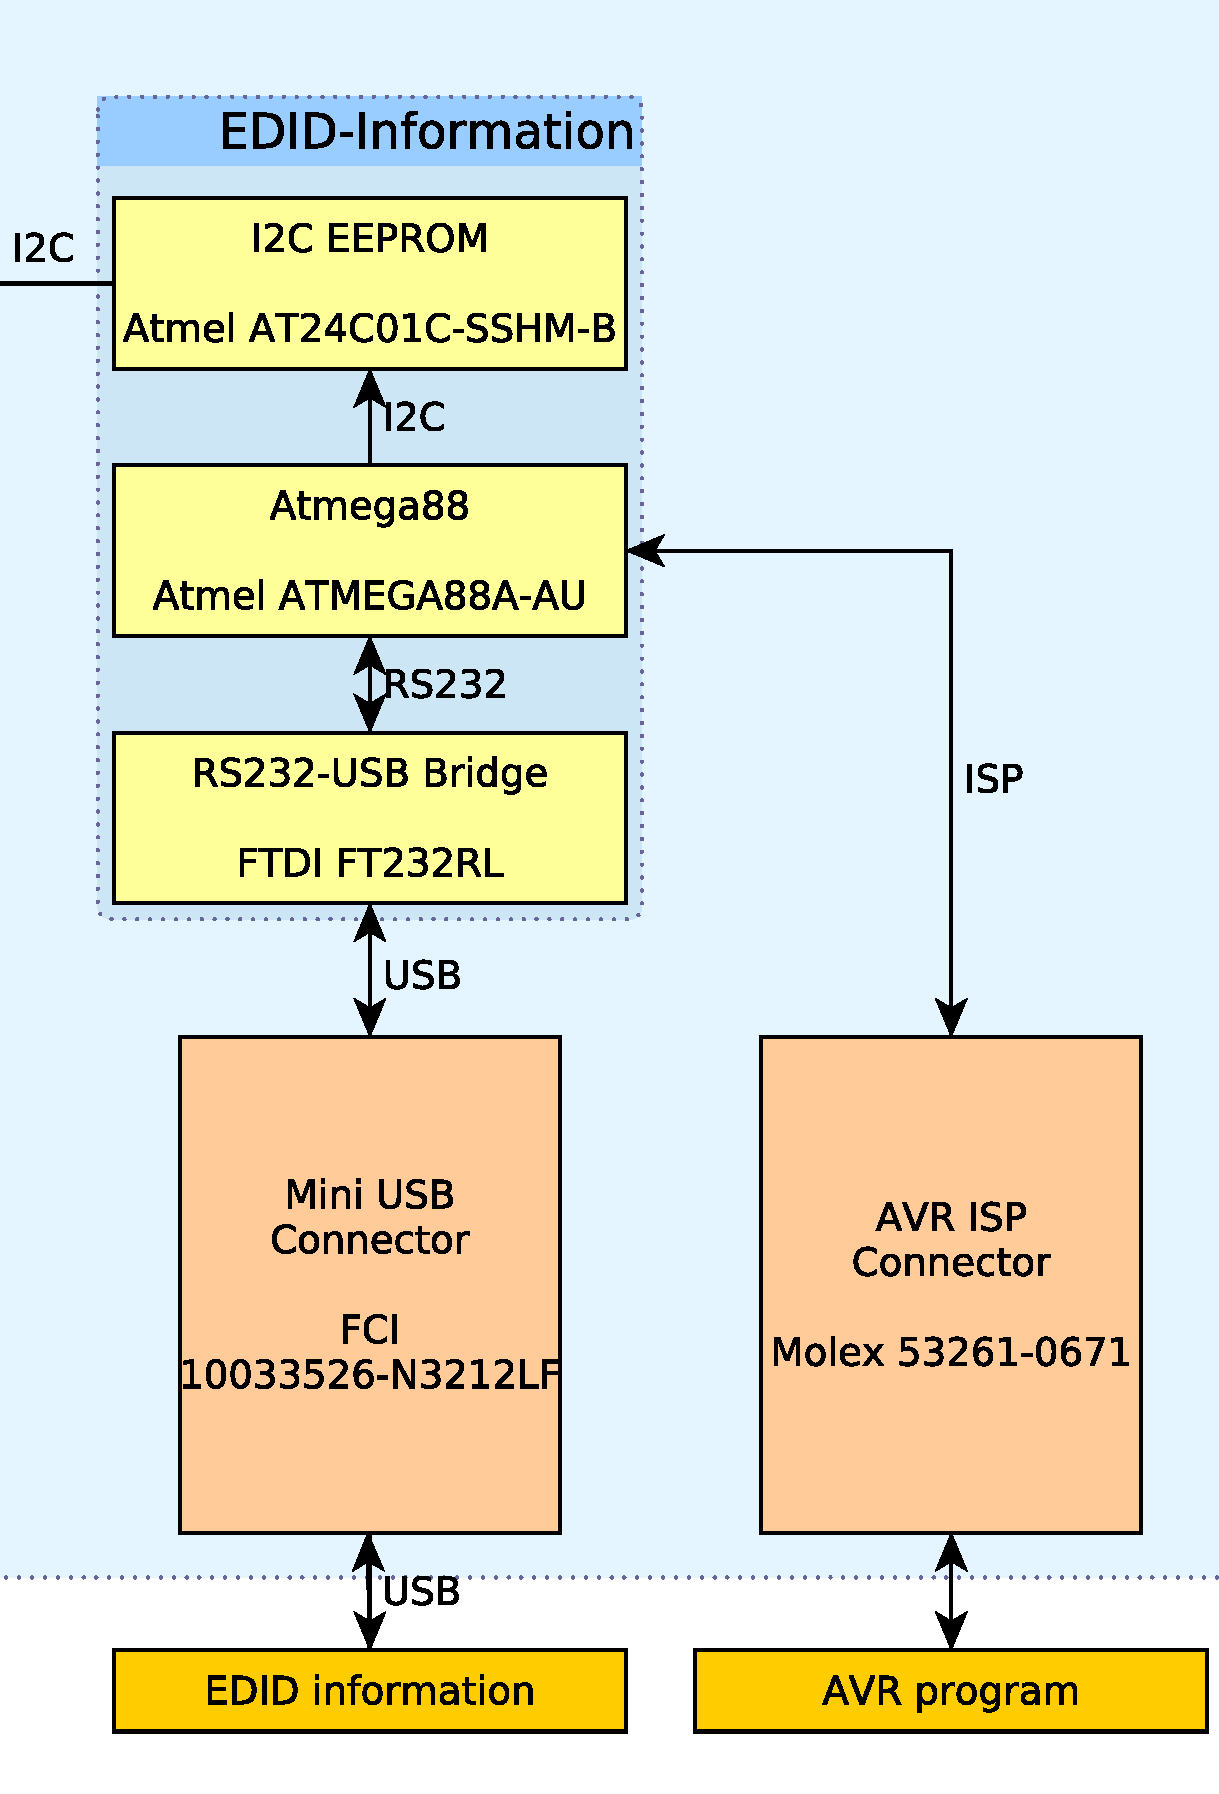
\includegraphics[width=0.6\textwidth]{TeilB/EDID.pdf}}
    \caption{EDID: Blockschaltbild}
    \label{fig:teilb_edid_blockschaltbild}
\end{figure}\\
Als externe Schnittstellen stehen eine USB-Buchse und ein ISP-Stecker\footnote{ISP: In System Programmer - Schnittstelle um den Prozessor im eingebauten Zustand zu programmieren} für den Prozessor zur Verfügung. Die RS232-UART-Bridge stellt die Kommunikation mit dem PC her, indem diese die serielle Schnittstelle des AVRs in USB-Signale umwandelt. Dies ist notwendig, da heutzutage kaum mehr echte serielle Schnittstellen in Computern verbaut sind. Gerade im embedded Bereich ist die Verwendung der seriellen Schnittstelle aufgrund seiner einfachen Bedienung sehr beliebt, weshalb Lösungen mittels USB-Konvertern quasi zum Standard gehören. Der Prozessor selbst ist durch einen ATMEGA88 realisiert, und beschreibt das $I^2C$-EEPROM mit einem in der Software hinterlegten Protokoll. 
\refa{fig:teilb_edid_usb_sch} zeigt die USB-Bridge mit dem USB-Stecker und dem Baustein \code{FT232RL} von FTDI, der die Konversion durchführt. Die differentiellen USB-Signale \code{USB_D+} und \code{USB_D-} sind mit dem Eingang des Bausteins verbunden. An den Ausgängen sind die seriellen Signale \code{FTDI_RX} und \code{FTDI_TX}. Diese Leitungen stellen die ein- beziehungsweise ausgehenden Signale zum und vom Prozessor dar.
\begin{figure}[htp]
	\center
	\fbox{	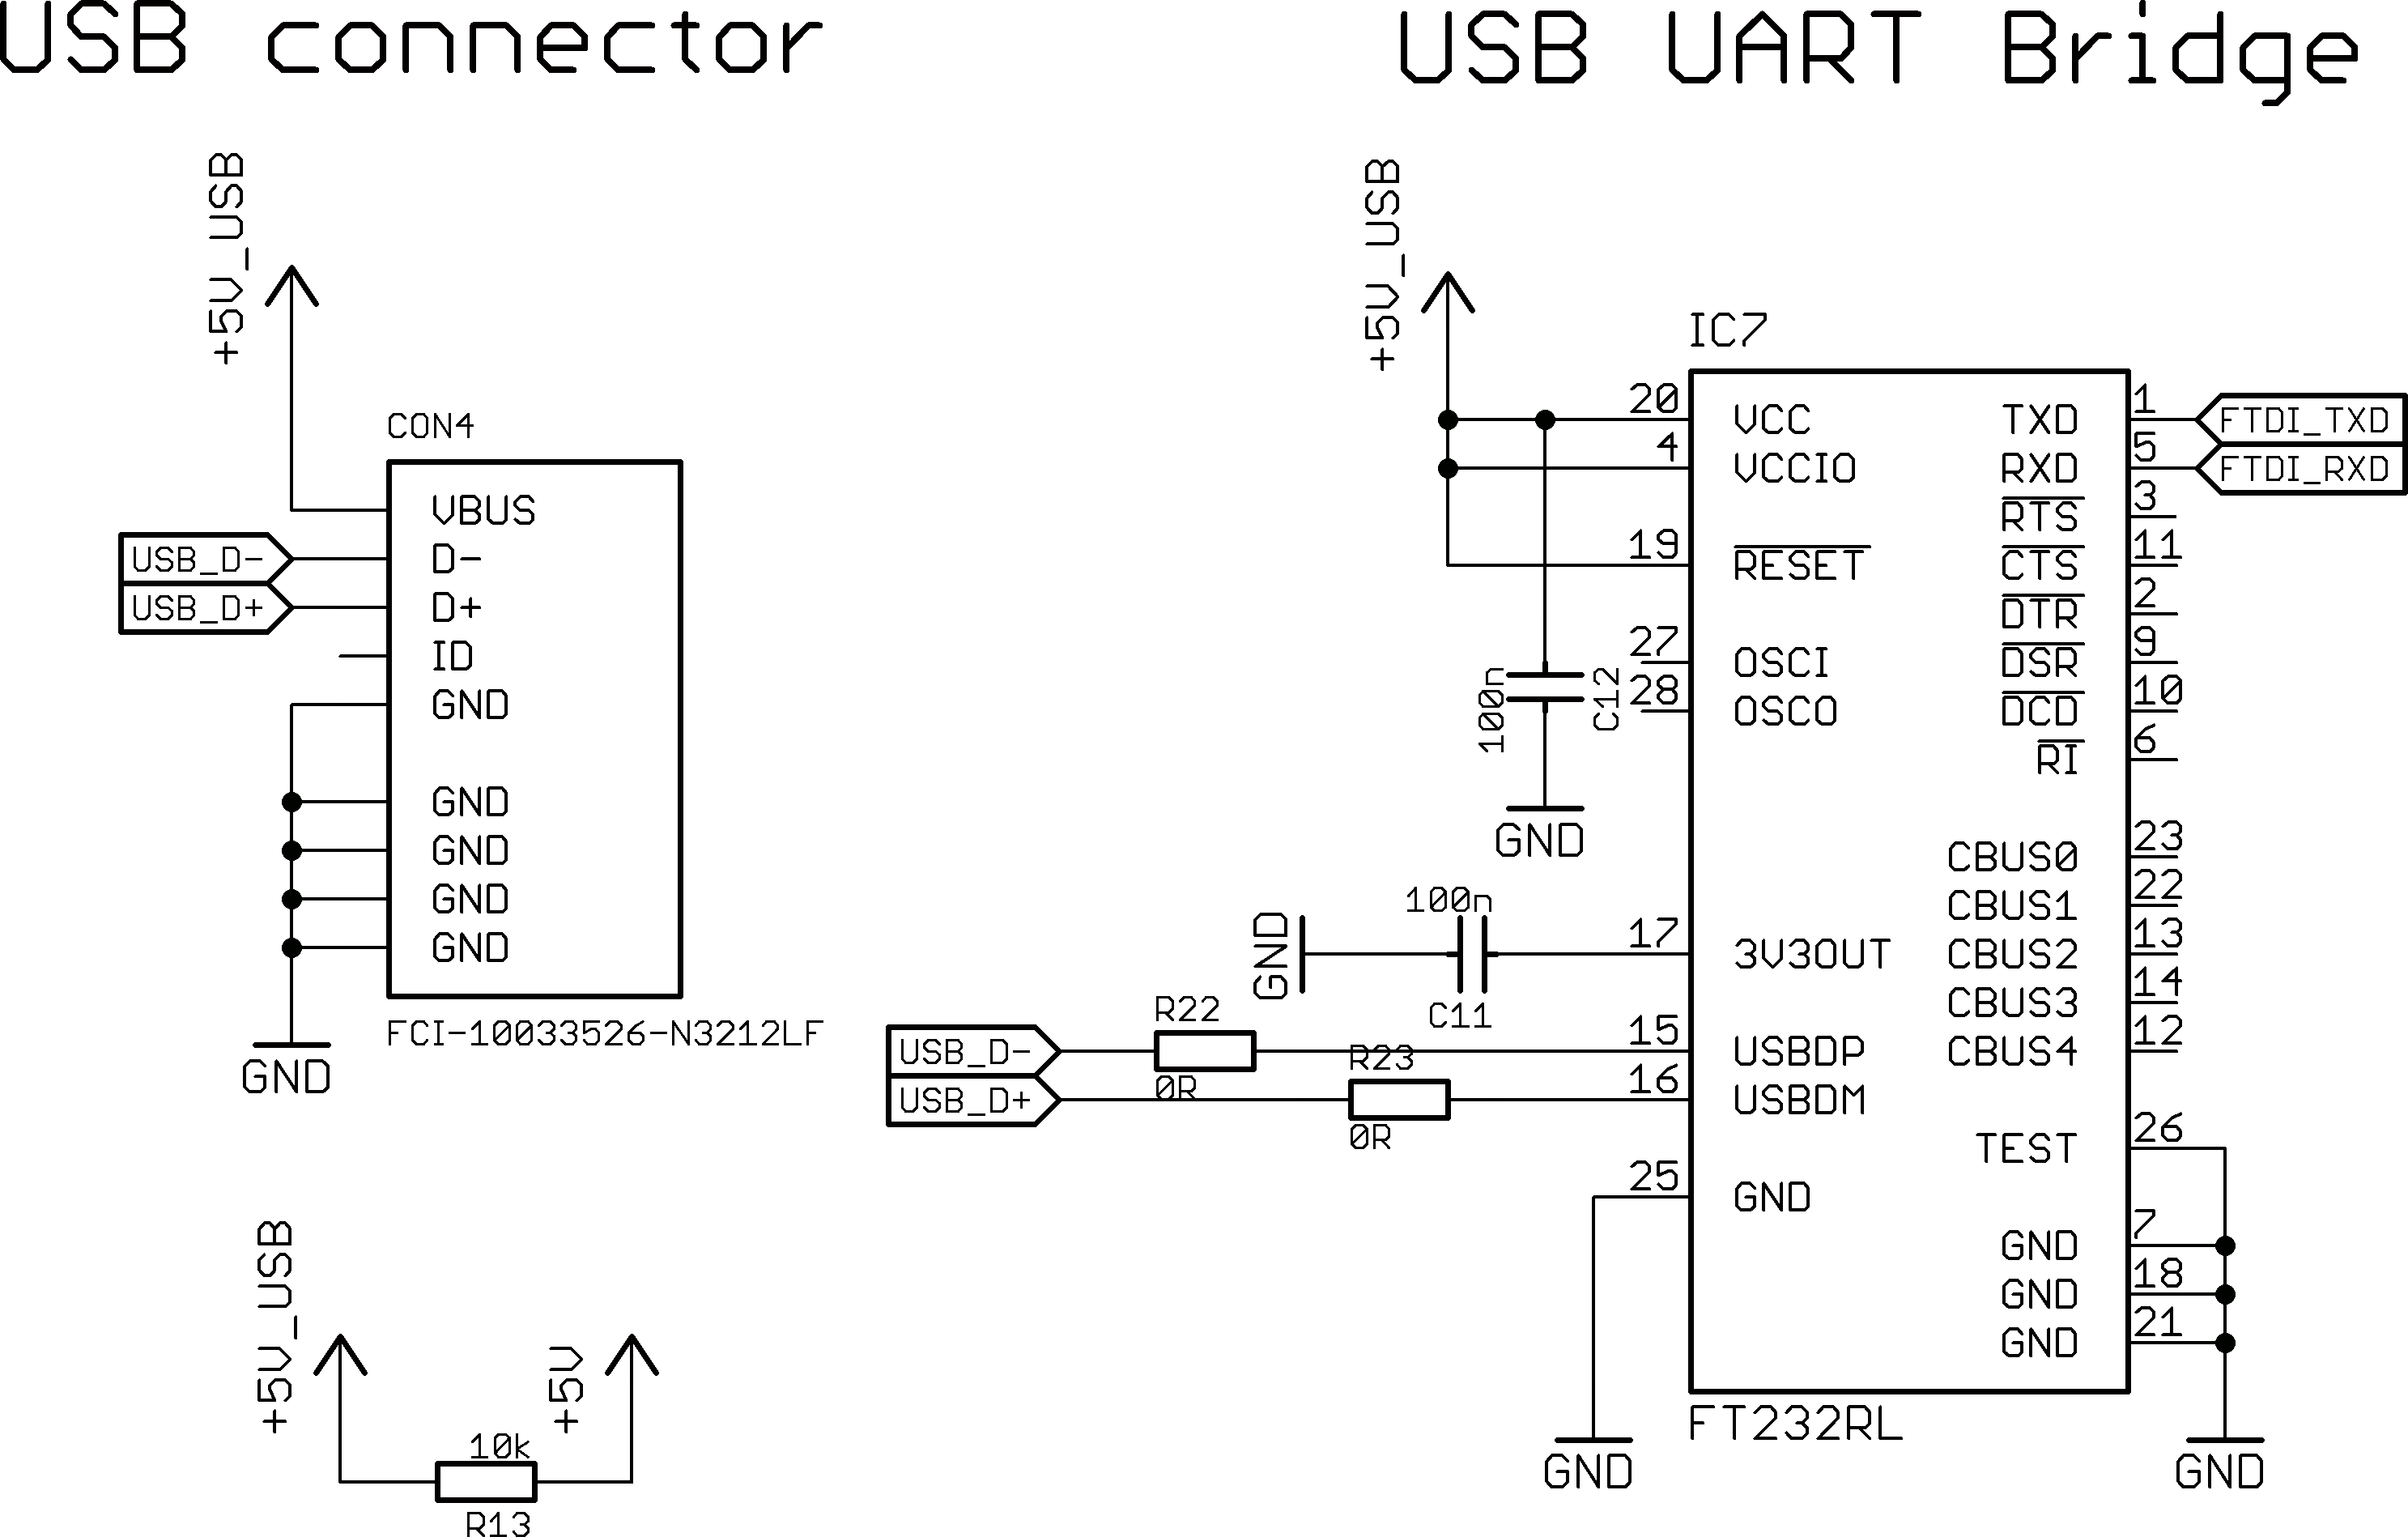
\includegraphics[width=0.8\textwidth]{TeilB/usb_sch.png}}
    \caption{EDID: USB-Bridge Schaltplan}
    \label{fig:teilb_edid_usb_sch}
\end{figure}\\
\refa{fig:teilb_edid_avr_sch} zeigt die Beschaltung des AVRs \code{IC6} und des EEPROMs \code{IC4}. Neben der Grundbeschaltung mit Quarz und Reset-Pin am AVR gehen die $I^2C$-Signale \code{EDID_SCL} und \code{EDID_SDA} an die Pins des EEPROMs. Das EEPROM bietet die Möglichkeit einen Schreibschutz aktiv zu schalten. Dieser kann mit dem Jumper \code{JP5} ein- und ausgeschaltet werden. Zum Programmieren des Prozessors ist der ISP-Stecker mit den entsprechenden Signalen verbunden. Um die Bauform recht gering zu halten sind alle Komponenten als SMD-Varianten gewählt - so auch der ISP-Stecker \code{CON5}. Um die 128 Byte großen EDID-Daten vollständig aufnehmen zu können ist das entsprechend gleichgrosse EEPROM \code{AT24C01C} in Verwendung. \\
Neben der reinen Funktion als Programmiergerät für das EEPROM bietet die Schaltung noch die Möglichkeit ein PWM-Signal auszugeben, welches zum Dimmen der Hintergrundbeleuchtungen der Displays verwendet werden kann. Hierzu ist ein Potentiometer mit dem Signal \code{AVR_PWM_ADC} an einem Analog-Eingang des AVRs verbunden, der es ermöglicht die Spannung im Bereich zwischen +5V und 0V zu messen. Je nach gemessener Spannung am Potentiometer kann ein PWM-Signal \code{AVR_PWM} ausgegeben werden, wobei beispielsweise +5\,V 100\%  und +2.5\,V 50\% Helligkeit bedeuten. Liegen 0V am Eingang an, so wäre die Hintergrundbeleuchtung komplett ausgeschaltet, wobei sich das PWM-Signal stufenlos im gültigen Wertebereich einstellen lässt. 
\begin{figure}[htp]
	\center
	\fbox{	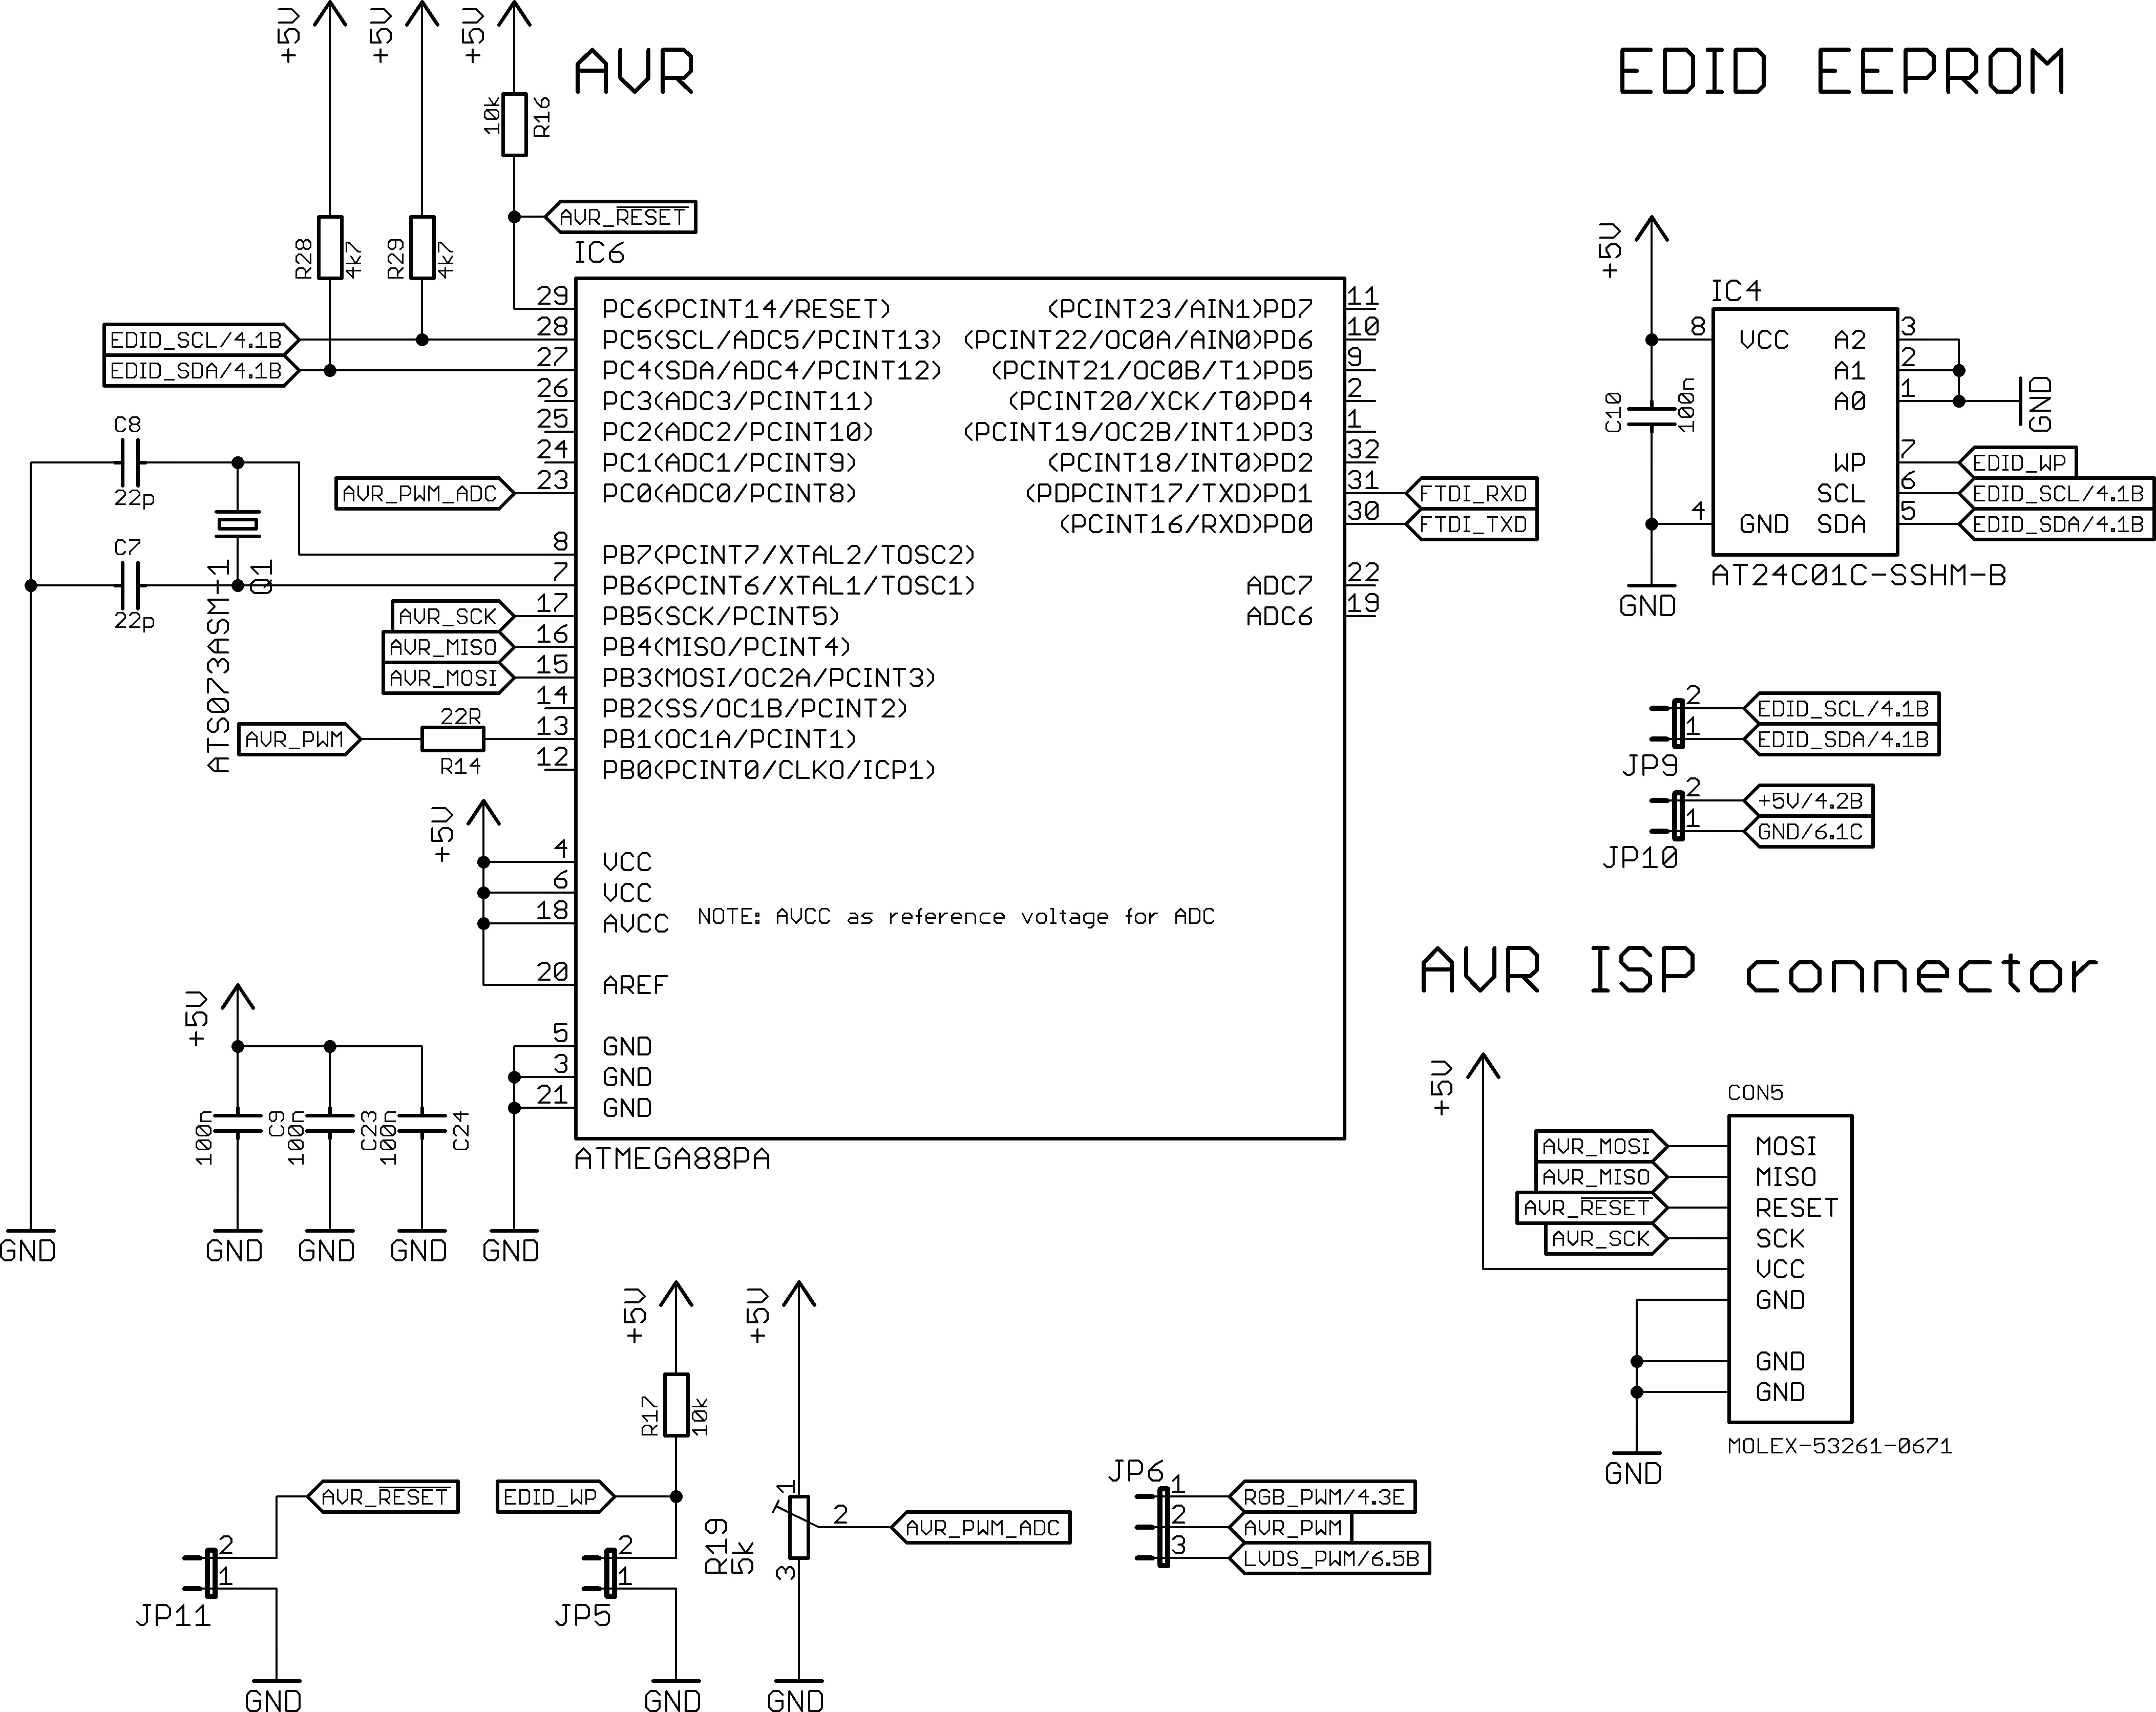
\includegraphics[width=1\textwidth]{TeilB/avr_sch.png}}
    \caption{EDID: AVR Schaltplan}
    \label{fig:teilb_edid_avr_sch}
\end{figure}\\
Der einzige kritische Aspekt beim Layout des Funktionsblocks ist der eingenommene Raum auf der Platine. Da hier weder mit schnellen Signalen noch hohen Strömen gearbeitet wird, kann die Leitungsführung platzoptimiert durchgeführt werden. Die Abbildungen \ref{fig:teilb_edid_pcb_top} und \ref{fig:teilb_edid_pcb_bot} zeigen das Layout auf dem Top- bzw. Bottom-Layer der Platine. In den Bildern sind die einzelnen Bereiche farblich und textuell markiert.

\begin{figure}[htbp]
        %\begin{center}
        \centering
        \begin{subfigure}[htp]{0.48\textwidth}
%                \fbox{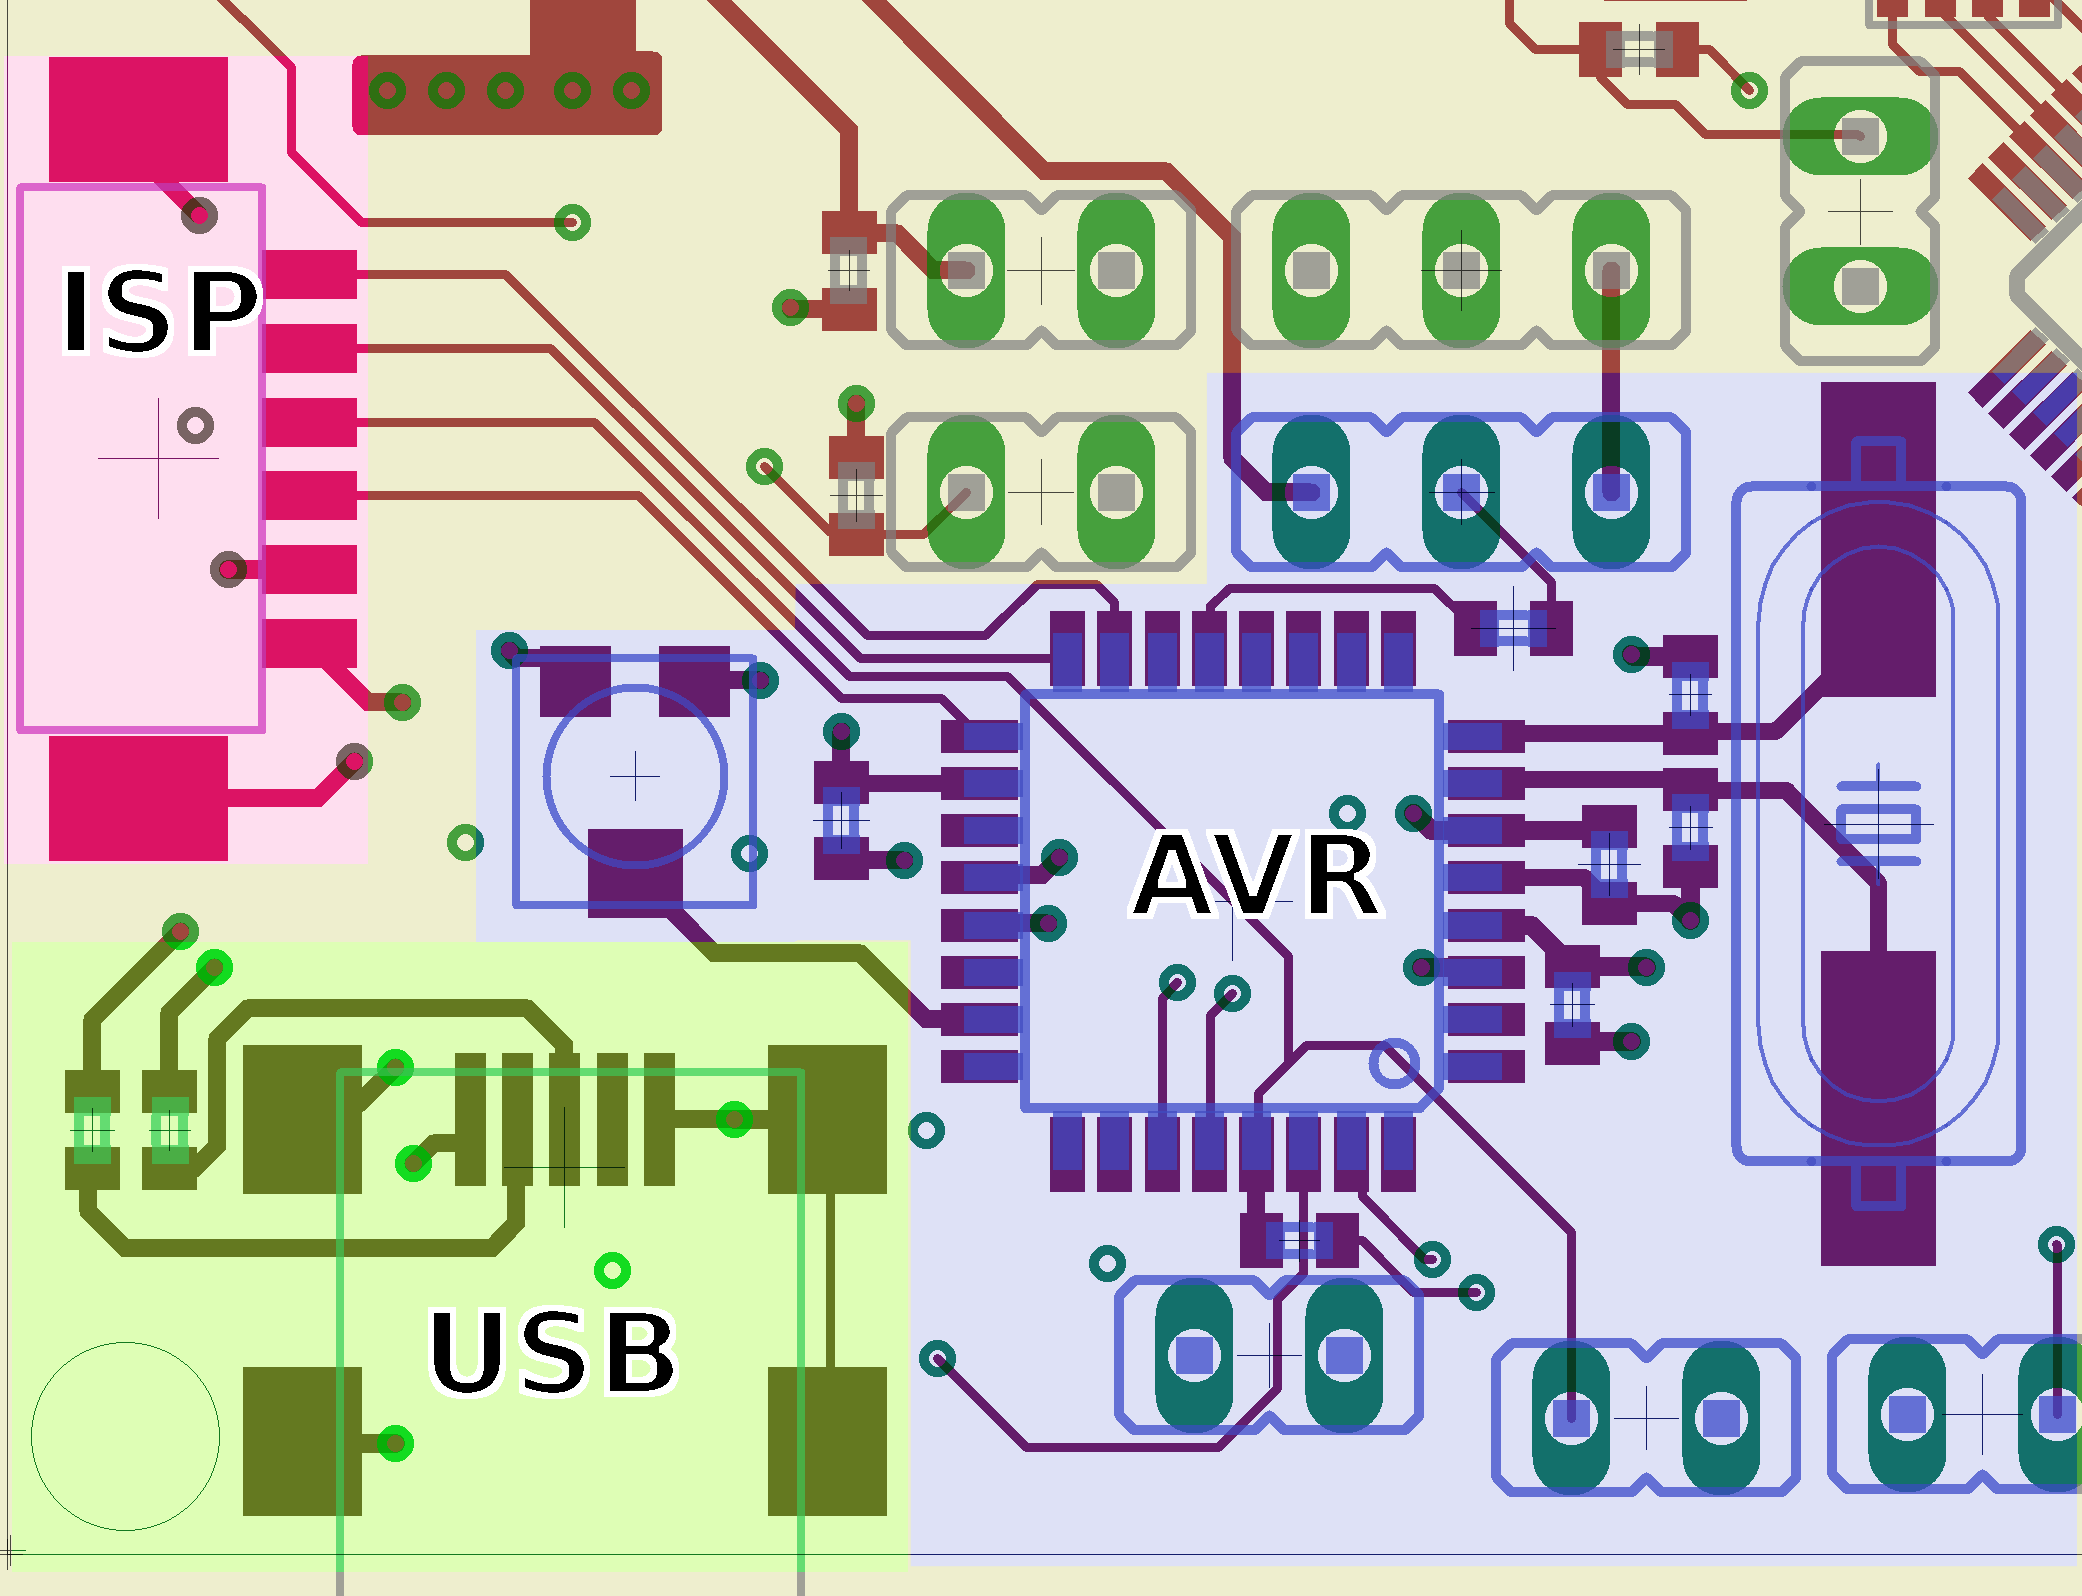
\includegraphics[width=1\textwidth]{TeilB/edid_pcb_top.png}}
                \fbox{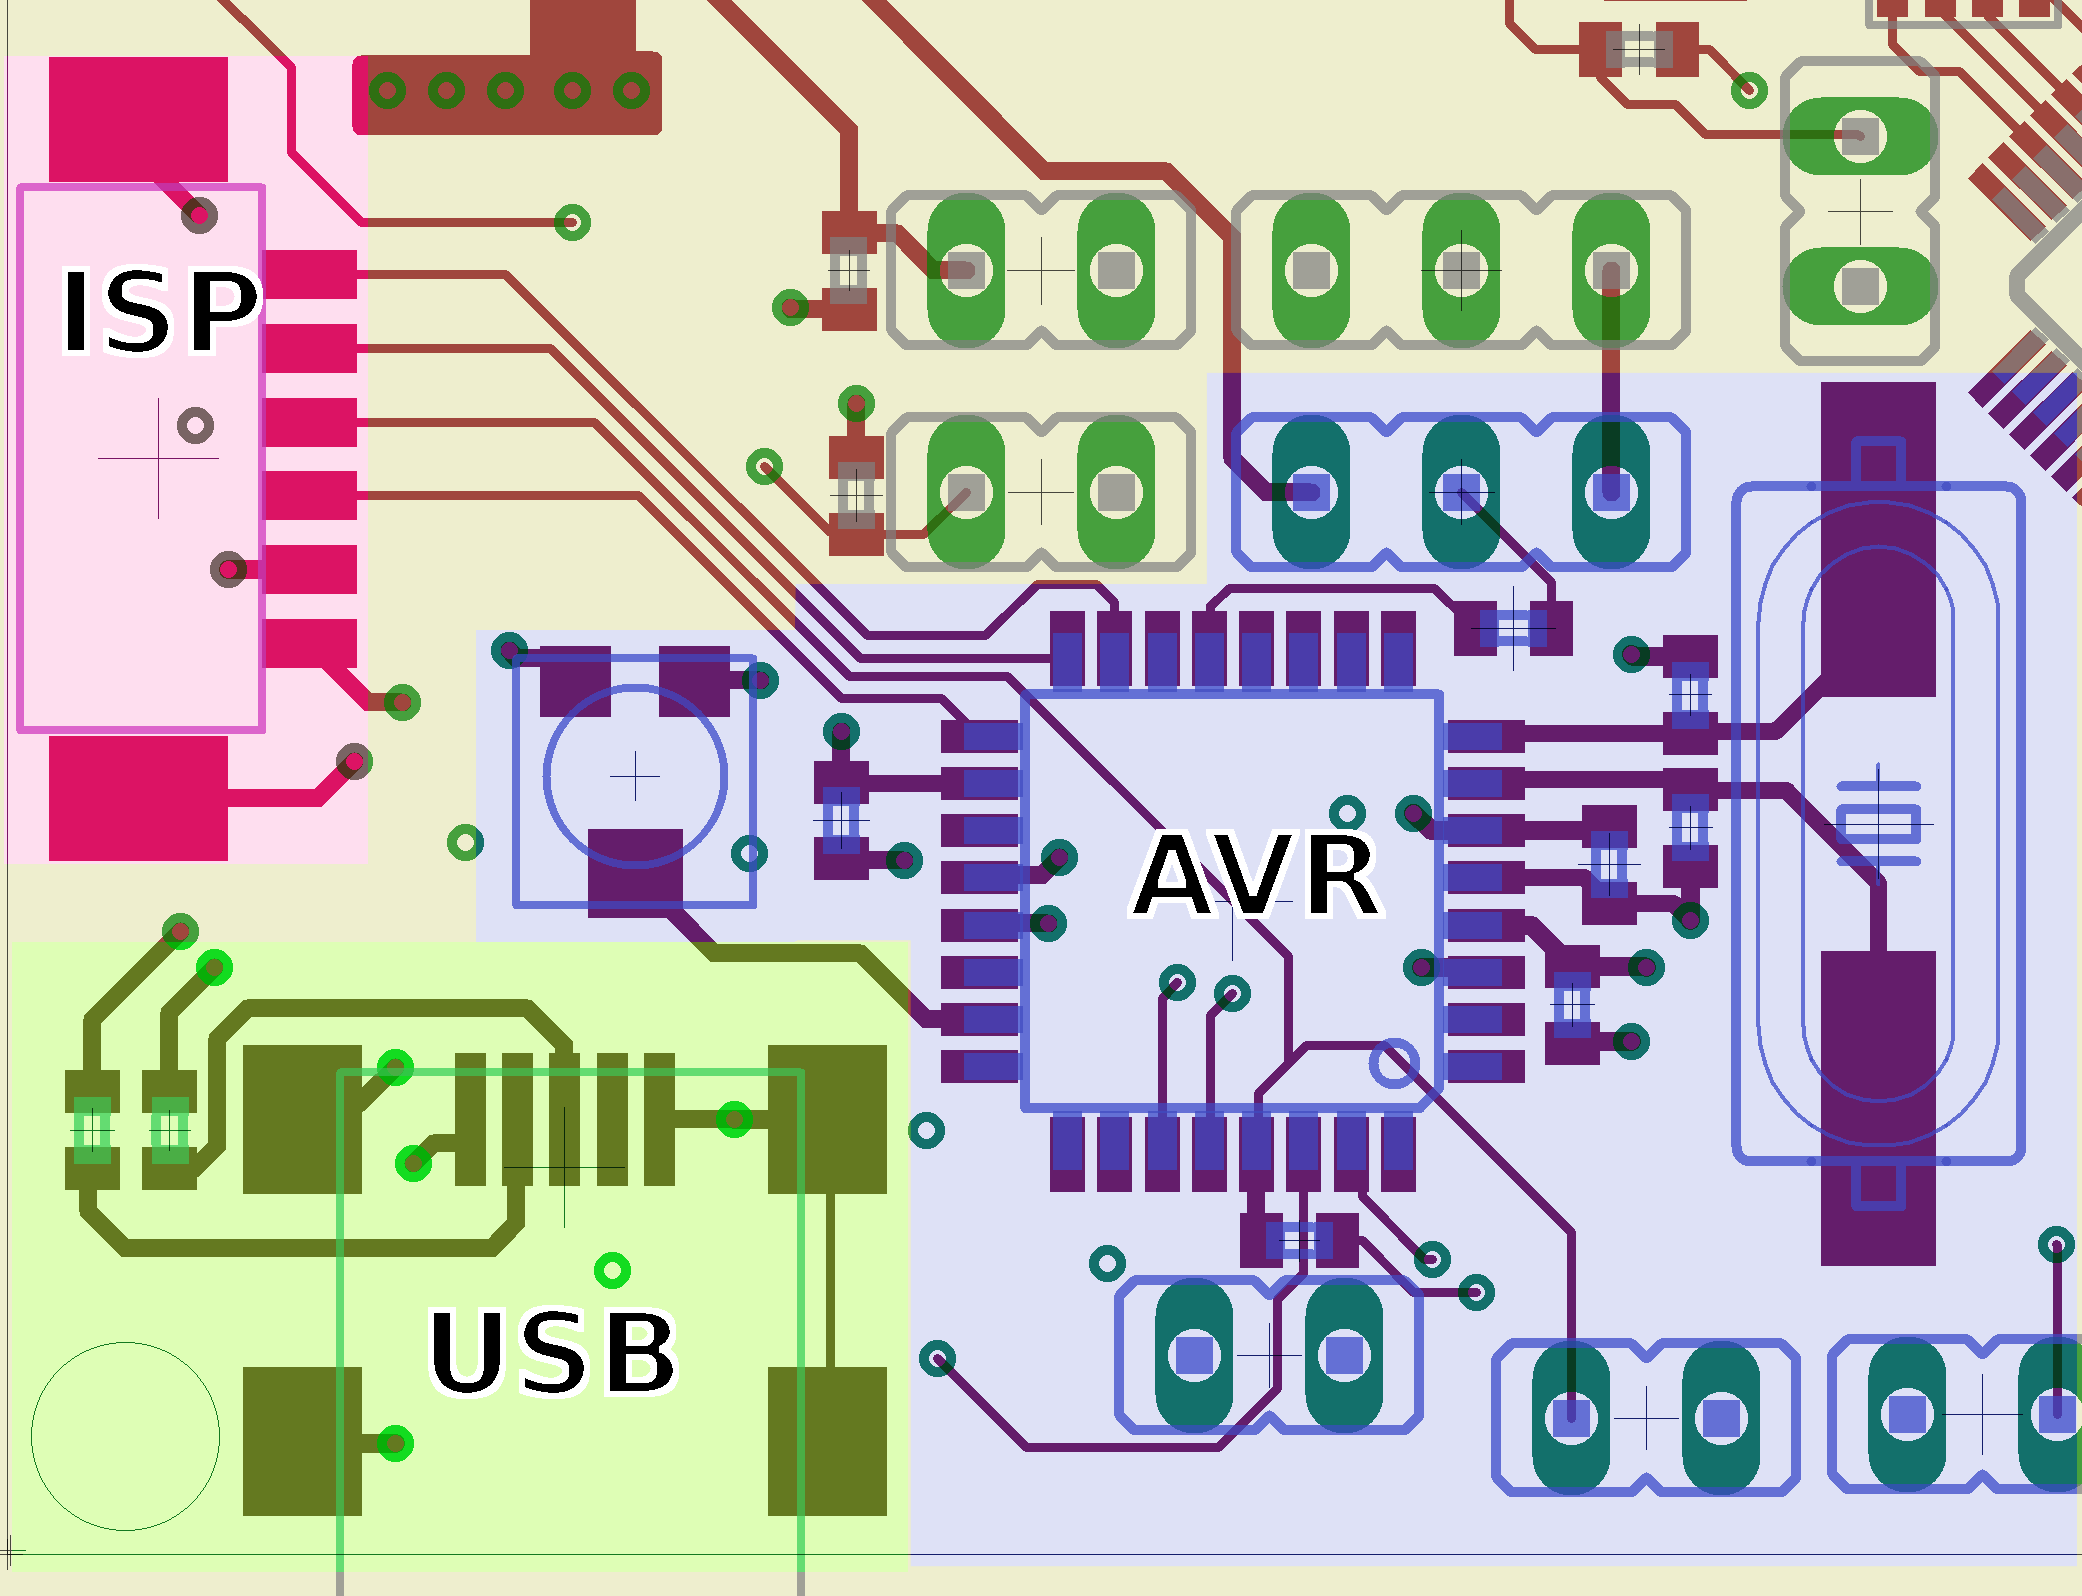
\includegraphics[height=5cm]{TeilB/edid_pcb_top.png}}
                \caption{Top Layer}
                \label{fig:teilb_edid_pcb_top}
        \end{subfigure}
\quad 
        \begin{subfigure}[htp]{0.48\textwidth}
%               \fbox{ 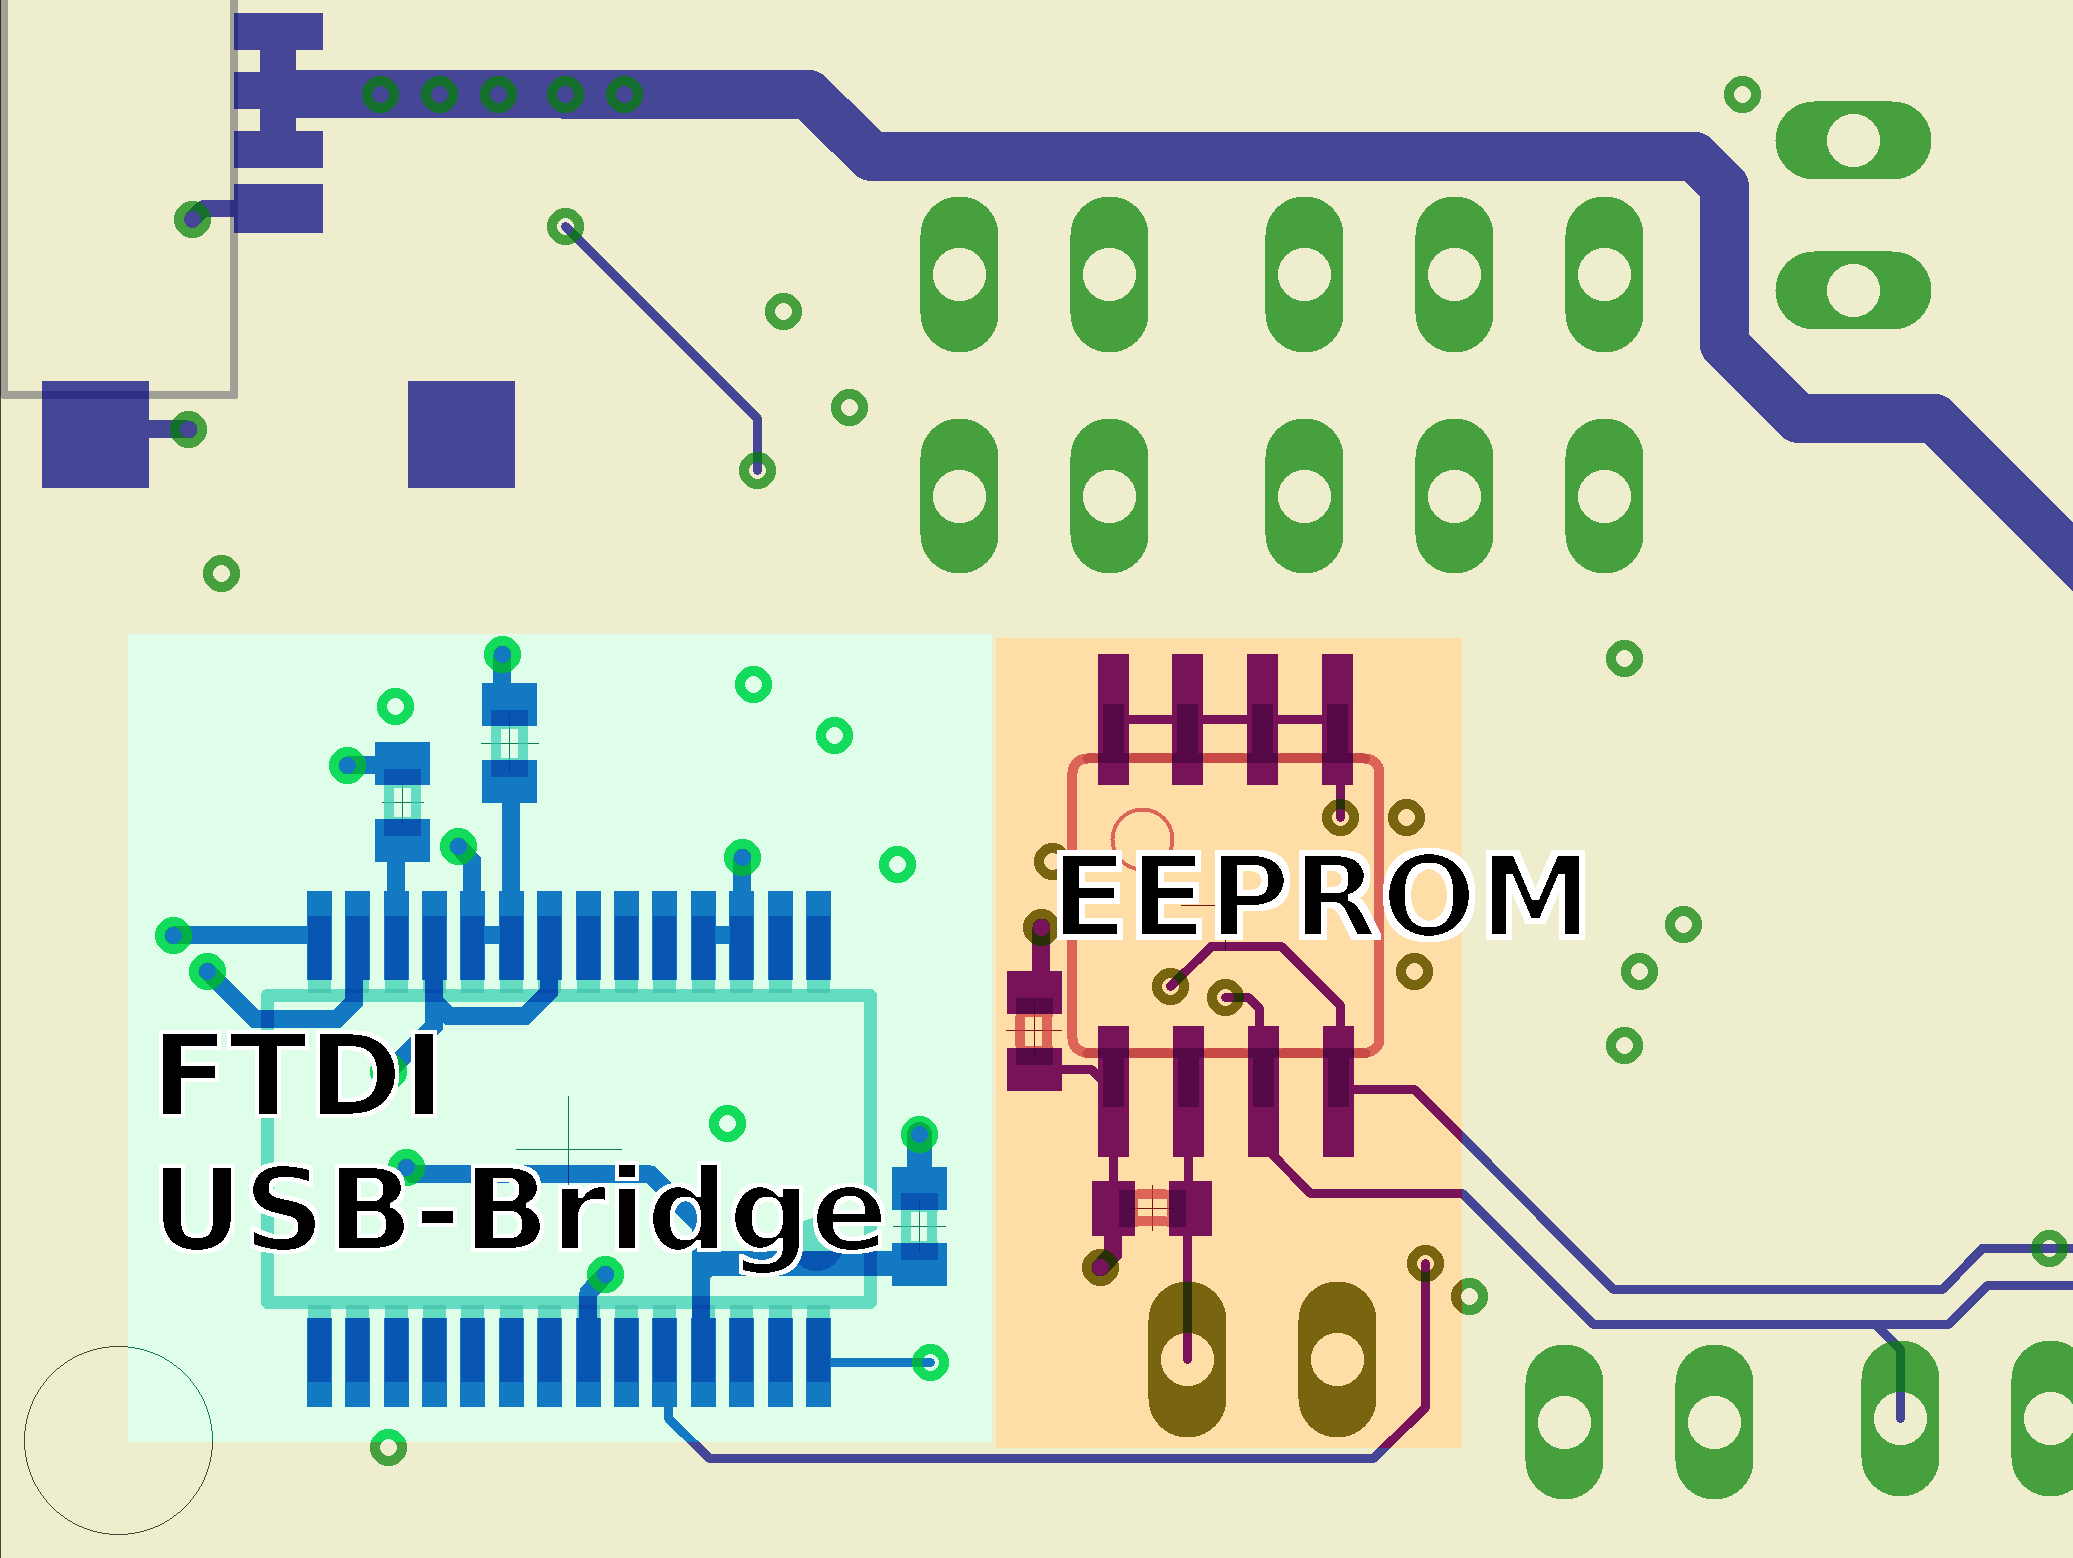
\includegraphics[width=1\textwidth]{TeilB/edid_pcb_bot.png} }              		
               \fbox{ 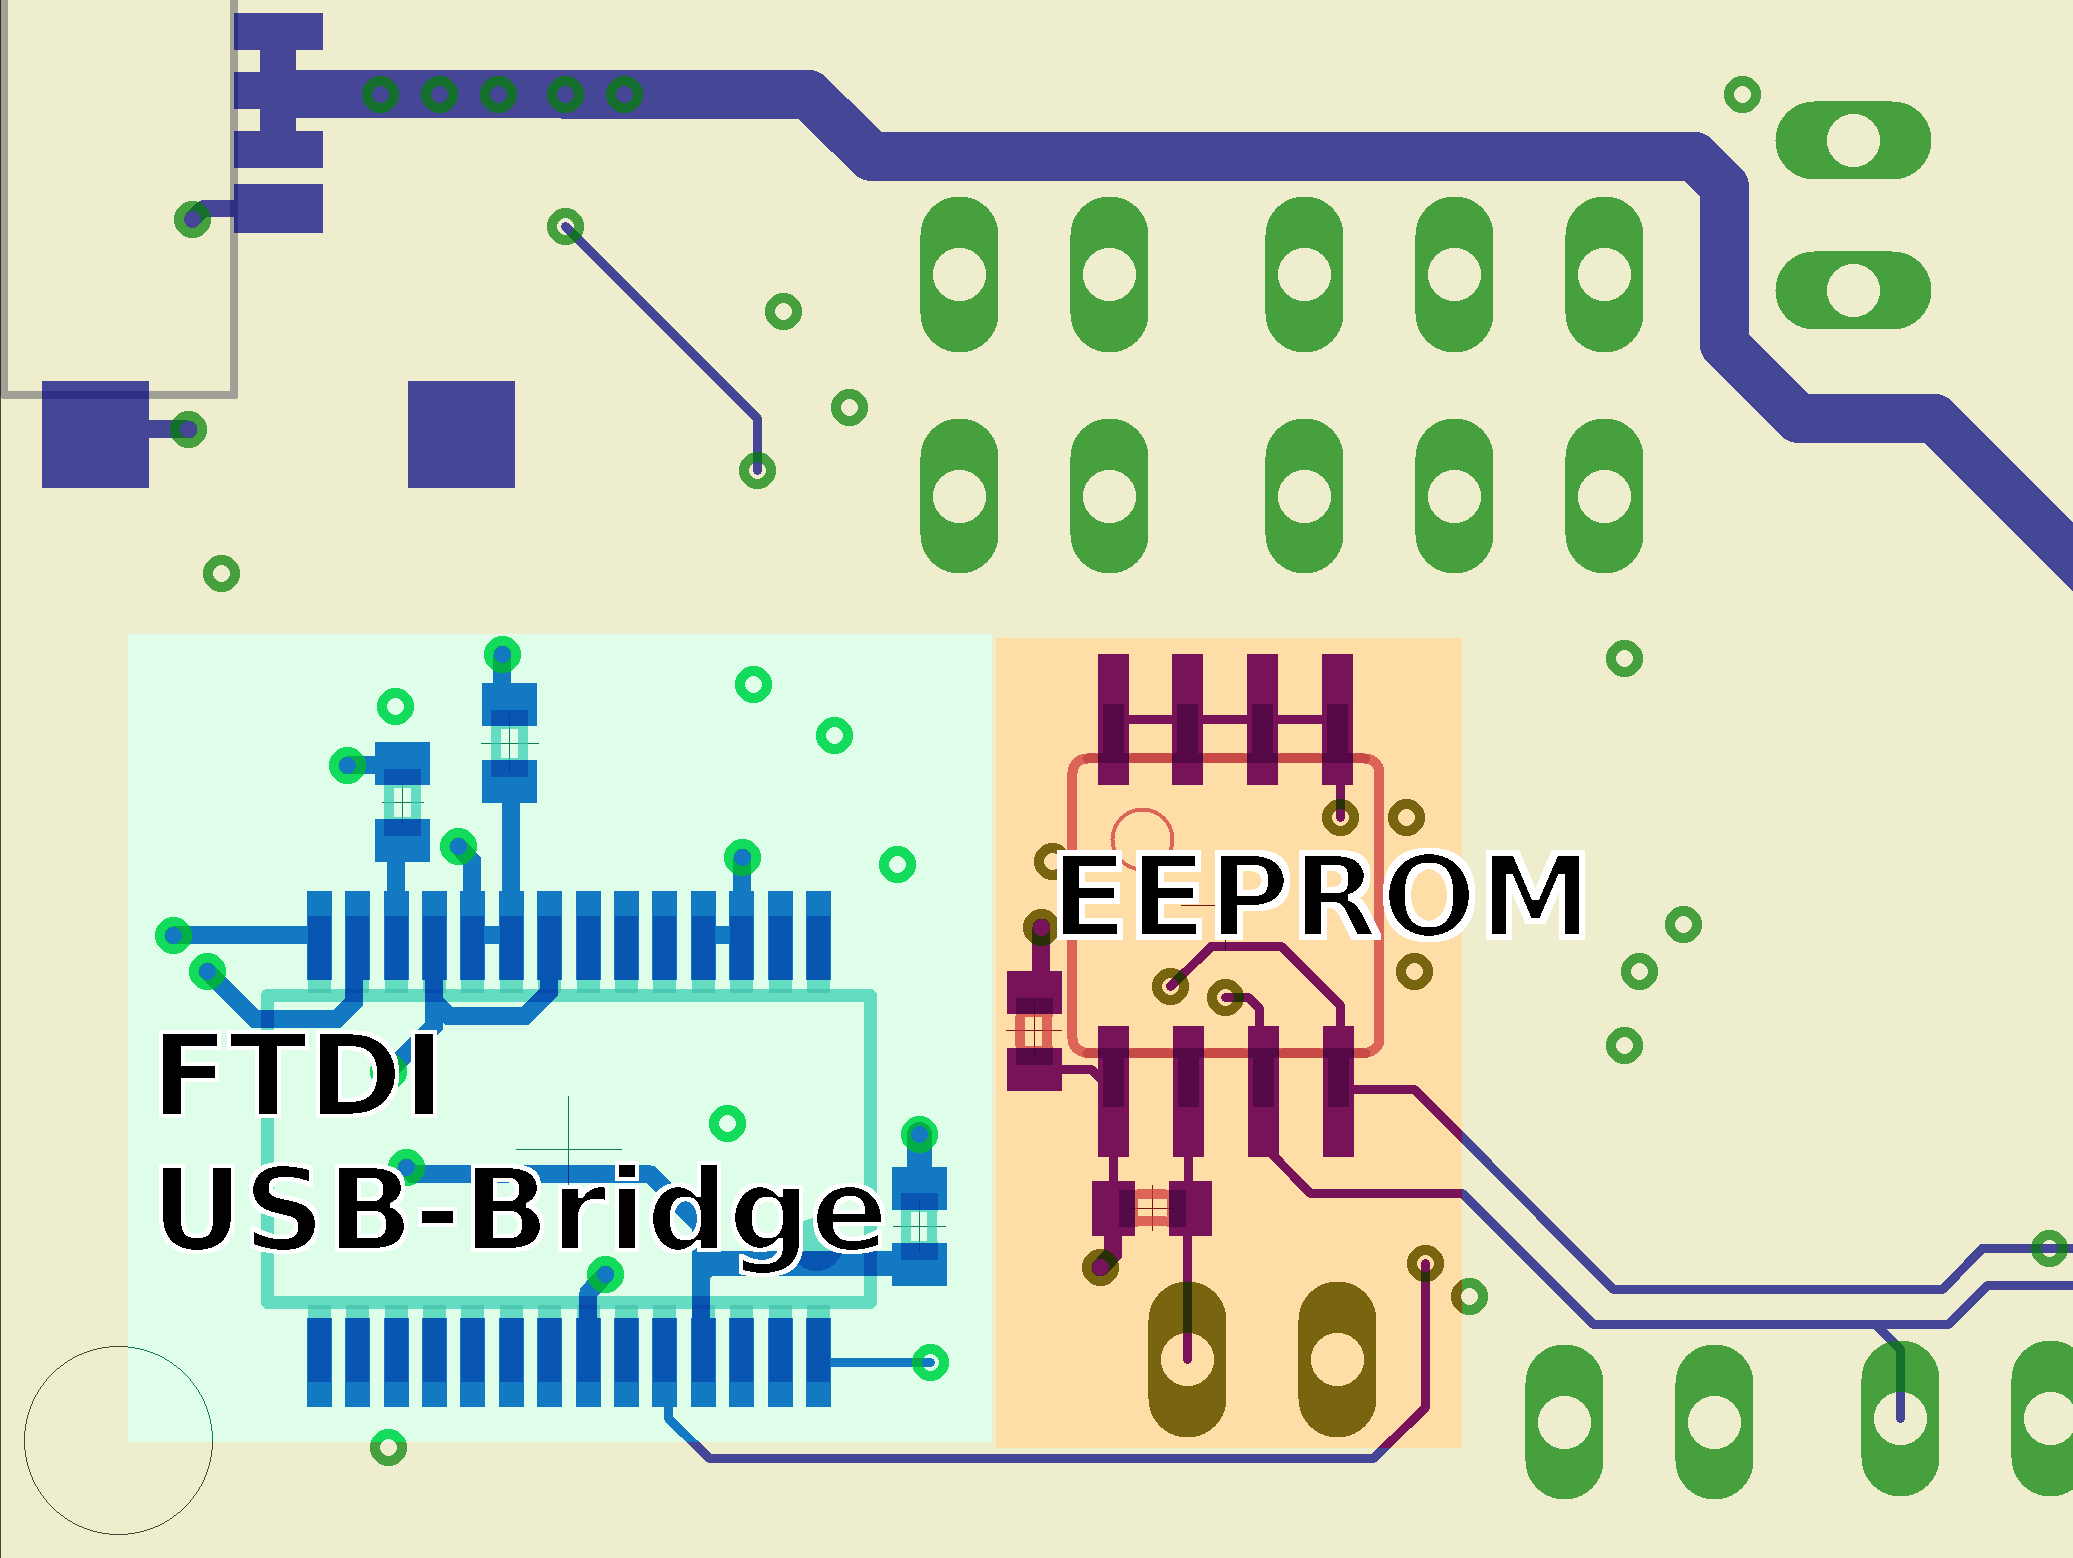
\includegraphics[height=5cm]{TeilB/edid_pcb_bot.png} }              		
		\caption{Bottom Layer}
                \label{fig:teilb_edid_pcb_bot}
        \end{subfigure}
		%\end{center}
        \caption{EDID Baugruppe}
        \label{fig:teilb_edid_pcb}
\end{figure}


\subsection{Spannungsversorgung}
Im Projekt werden drei verschiedene Spannungen verwendet. \refa{fig:teilb_supply} zeigt, wie die Spannungen voneinander abhängen und welche Baugruppe wie versorgt wird. 
\begin{figure}[htp]
	\center
	\fbox{	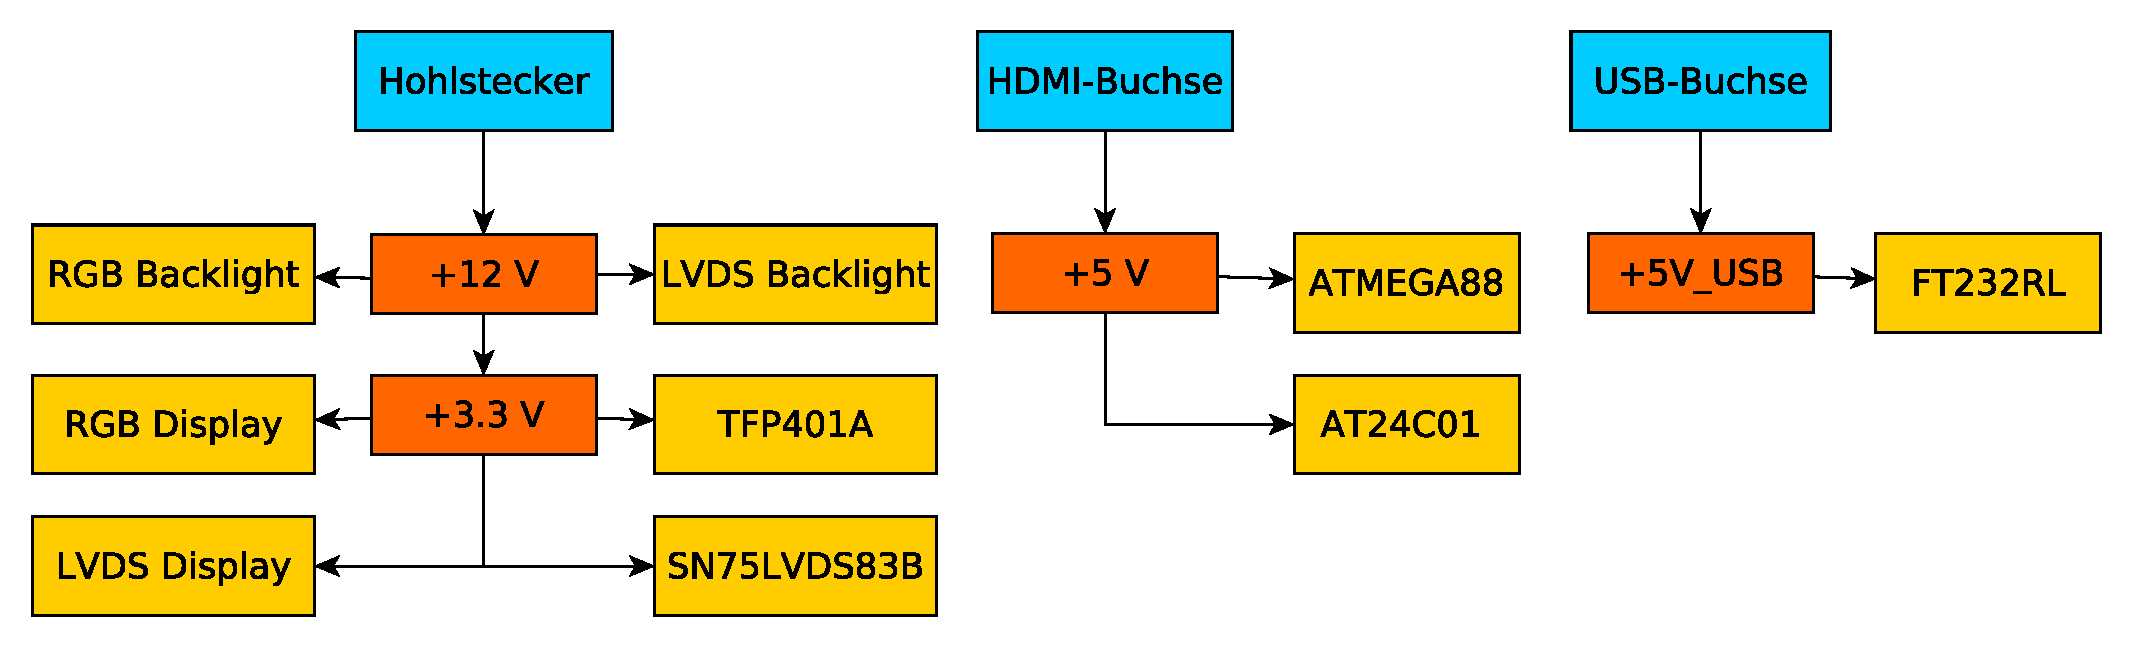
\includegraphics[width=1\textwidth]{TeilB/Supply.pdf}}
    \caption{Spannungsversorgung Teil B}
    \label{fig:teilb_supply}
\end{figure}\\
Extern werden über einen Hohlstecker +12\,V eingespeist, die ihrerseits die Hintergrundbeleuchtungen der Displays sowie den Schaltregler für die +3.3\,V Erzeugung versorgt. Um der Hardware beim verpolten Einstecken des Versorgungssteckers keinen Schaden zuzufügen, ist ein Verpolschutz eingebaut. Dieser ist mittels eines P-Kanal MOSFET\footnote{MOSFET: Feldeffekt-Transistor} \code{T1} realisiert. Der Schaltplan des Verpolschutzes und der +3.3\,V-Versorgung ist in \refa{fig:3_3_supply} zu sehen.
\begin{figure}[htp]
	\center
	\fbox{	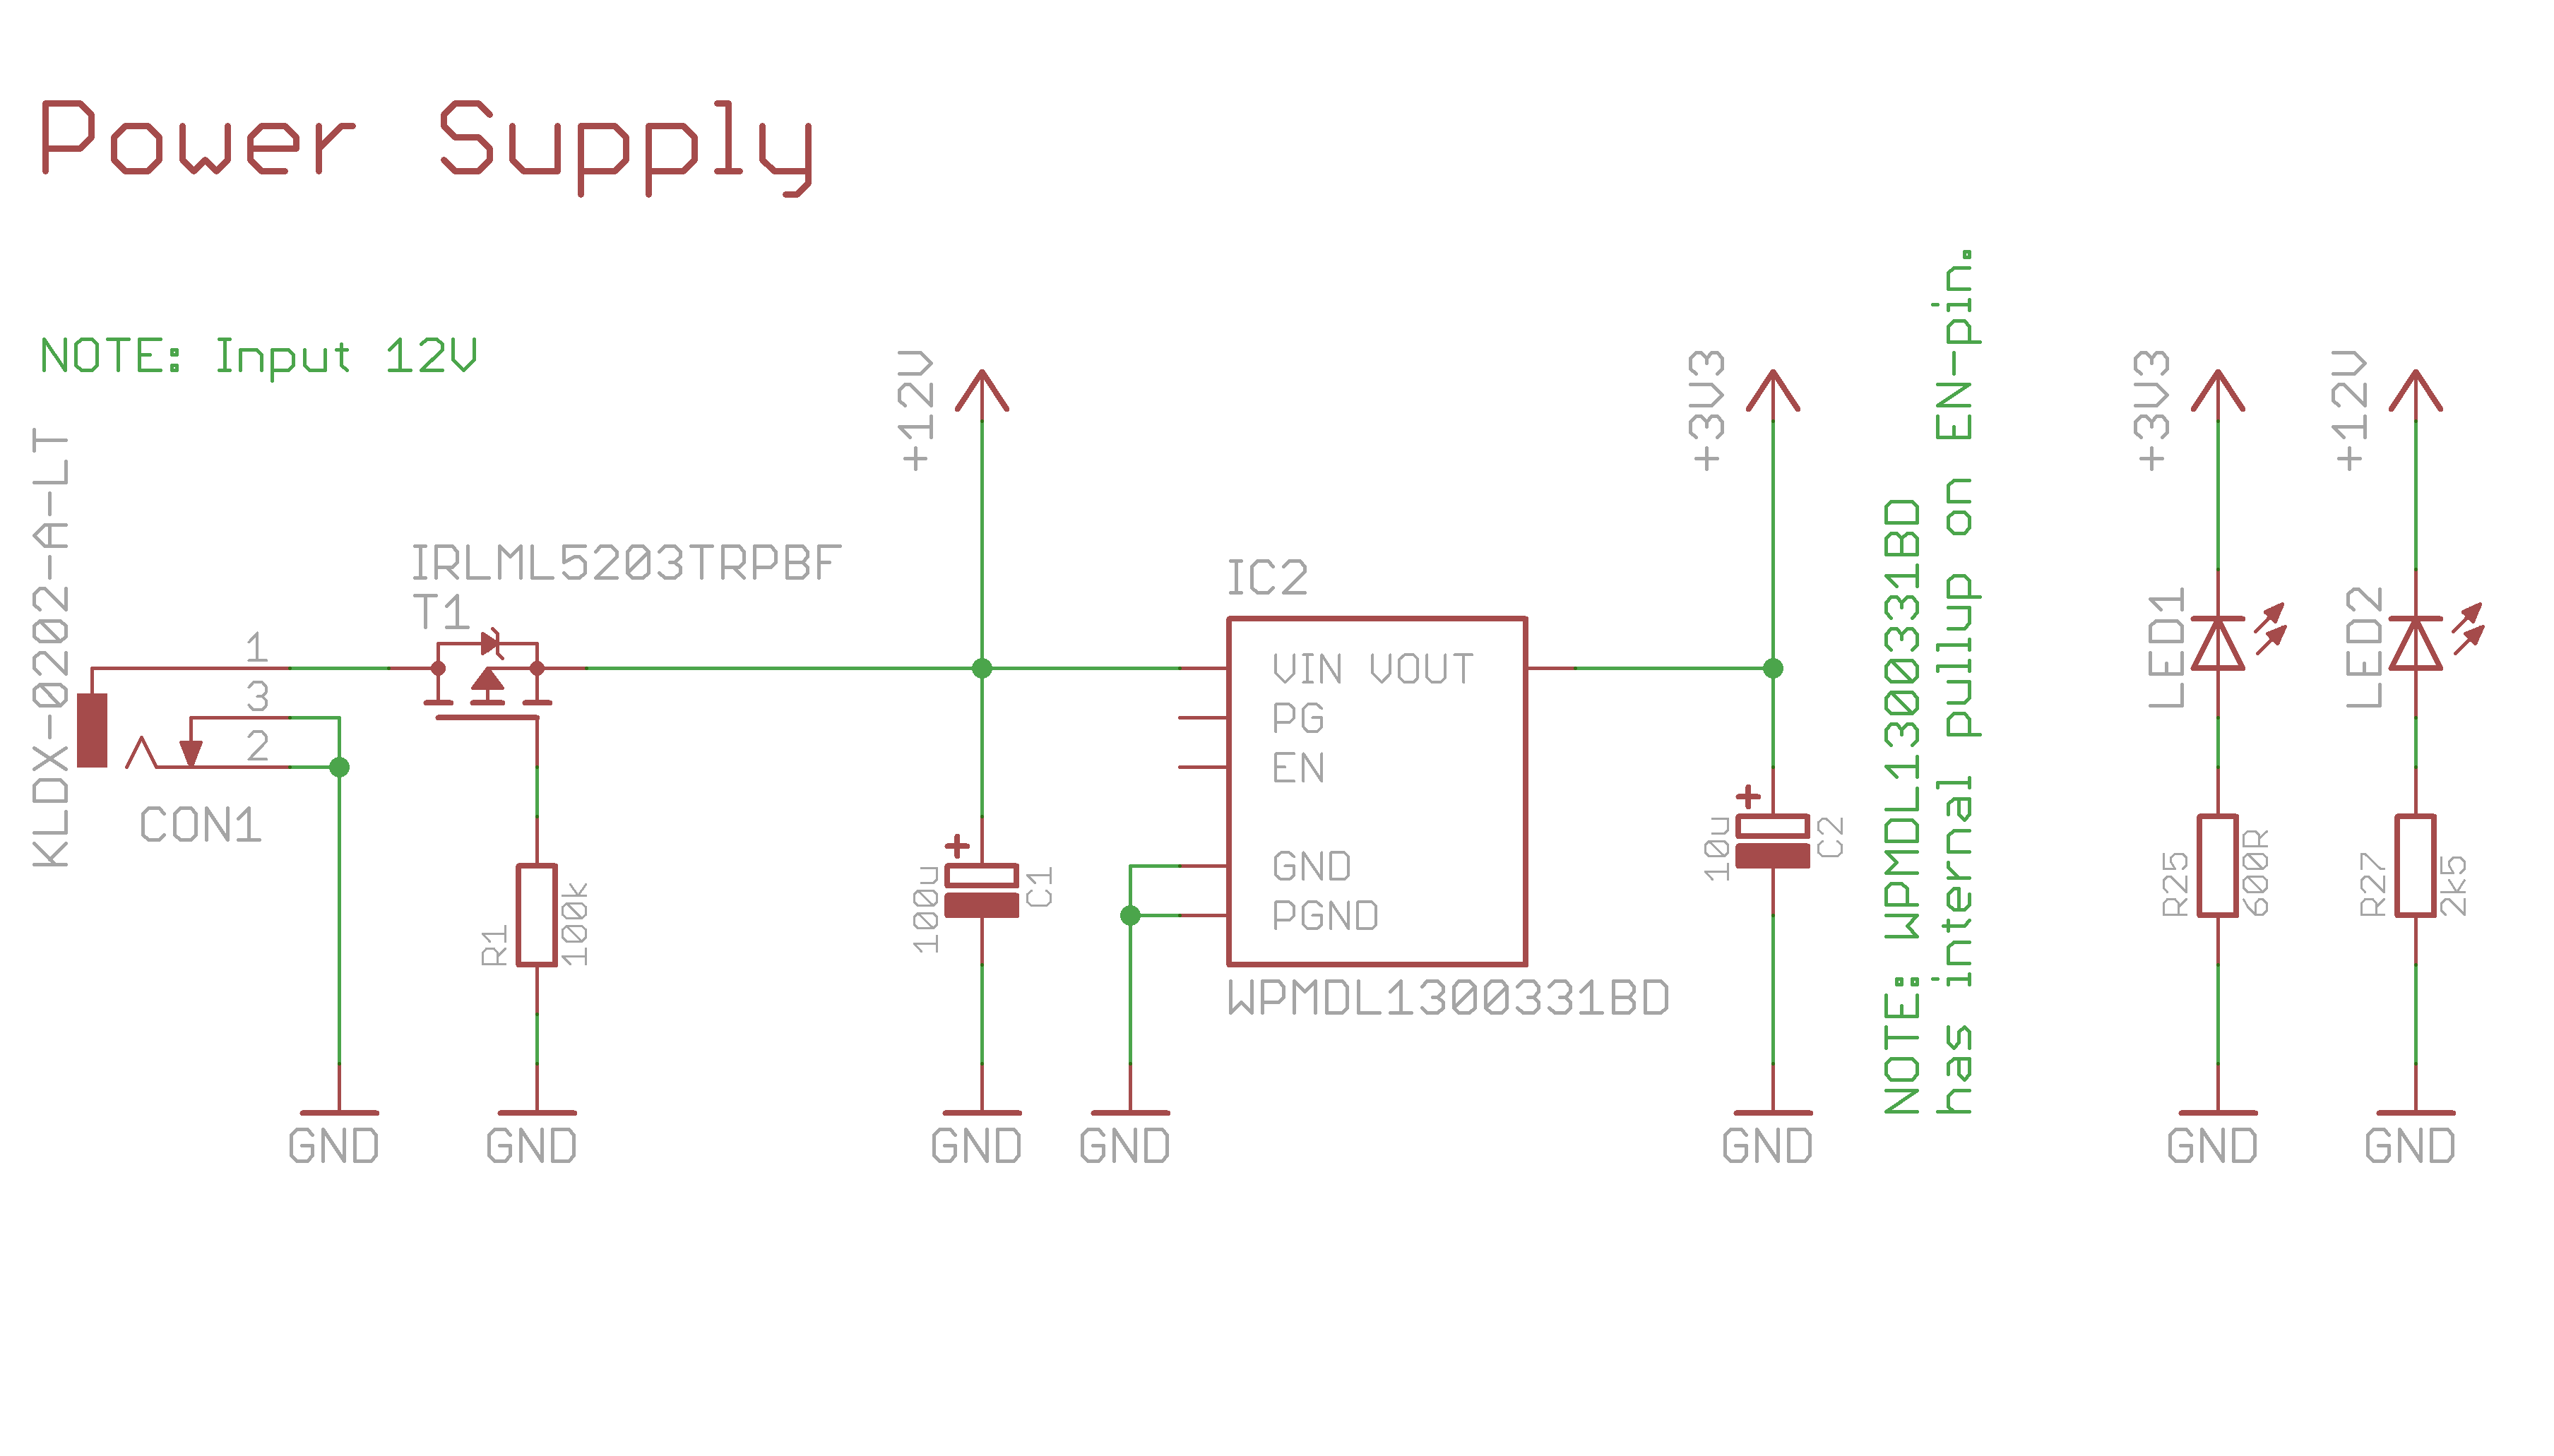
\includegraphics[width=1\textwidth]{TeilB/power_sup_sch.png}}
    \caption{Verpolschutz und Versorgungsspannung +3.3\,V}
    \label{fig:3_3_supply}
\end{figure}\\
Wird eine korrekt gepolte Spannung angelegt, leitet zuerst die Bulk-Diode des P-Kanal MOSFETs. Somit liegt die Eingangsspannung an Source an und die Bedingung ist erfüllt, dass die Source-Spannung um $U_{gsth}$ kleiner wird wird als die Gate-Spannung. Der Transistor leitet nun Strom. Wird aber eine verpolte Spannung angelegt, so sperrt die Bulk-Diode und der Transistor ist nicht in der Lage in einen leitenden Zustand zu gelangen (siehe \cite{Miller2010}). \refa{fig:verpolschutz_sim} zeigt ein Simulationsergebnis des Verpolschutz, bei dem im Wechsel +12\,V und -12\,V am Eingang angelegt werden. Die Grüne Kurve zeigt diese wechselnde Eingangsspannung, die Blaue die Spannung nach dem Verpolschutz. Zu sehen ist, dass sobald die Spannung negativ wird, der Transistor sperrt und die Spannung bei 0\,V liegt.
\begin{figure}[htp]
	\center
	\fbox{	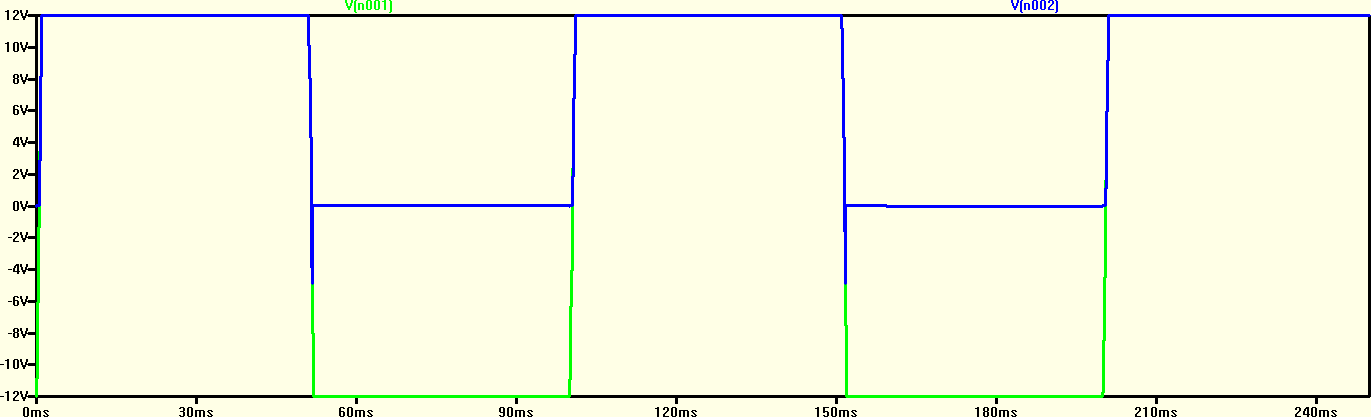
\includegraphics[width=1\textwidth]{TeilB/verpolschutz_messung.png}}
    \caption{Simulation des Verpolschutz}
    \label{fig:verpolschutz_sim}
\end{figure}\\

Die RGB-Bridge \code{TFP401A} sowie die LVDS-Bridge \code{SN65LVDS83B} werden mit +3.3\,V versorgt. Für die Erzeugung der +3.3\,V ist ein voll-integrierter Schaltregler \code{WPMDL1300331BD} von Würth Elektronik im Einsatz. Der Vorteil dieses Schaltreglers ist seine kompakte Bauform und dass keine weiteren externen Bauteile benötigt werden. Der Schaltregler liefert bei +3.3\,V bis zu 3\,A Strom (siehe \cite{Wuerth2013}, S. 4). Wie viel Strom die einzelnen Komponente innerhalb der +3.3\,V-Versorgung benötigen ist \reft{tab:3_3v_strom} zu entnehmen.
\begin{table}[h]
\begin{tabular}{|p{3cm}|p{5cm}|p{4.5cm}|}\hline
\rowcolor{TableBackgroundColor} 
   \textbf{Bauteil} & \textbf{Stromaufnahme} & \textbf{Quelle}	\\ \hline
    TFP401A & 370\,mA & \cite{TI2011}, S. 6\\ \hline
	SN65LVDS83B & 53.3\,mA & \cite{TI2011b}, S. 9\\ \hline
	LB070WV8-SL01 LVDS-Display & 403\,mA + 280\,mA = 683\,mA & \cite{LG2012}, S. 6f\\  \hline
	TY700TFT800480 RGB-Display & 125\,mA + 180\,mA = 305\,mA & \cite{Techtoys2012}, S. 3\\ \hline
\end{tabular}
\caption{Stromaufnahme der +3.3\,V-Versorgung}
\label{tab:3_3v_strom}
\end{table} \\
Wird unter Verwendung des RGB-Displays die LVDS-Bridge nicht auf der Platine bestückt, so errechnet sich die Stromaufnahme aus dem Verbraucht der RGB-Bridge und dem RGB-Display und beläuft sich auf  $370\,mA + 305\,mA = 675\,mA$. Wird die LVDS-Bridge bei gleichen Bedingungen bestückt, so ergibt sich eine maximale Stromaufnahme von $728\,mA$.\\
Im Falle der Verwendung des LVDS-Displays wird die RGB- sowie die LVDS-Bridge benötigt. Die errechnete maximale Stromaufnahme beläuft sich somit auf $370\,mA + 53\,mA + 683\,mA = 1106\,mA$. Die +3.3\,V-Versorgung ist somit für die Anwendung gut dimensioniert.\newline

Der ATMEGA sowie das EEPROM werden durch die HDMI-Buchse versorgt, da diese funktionieren müssen, sobald die Platine angesteuert wird. Laut Spezifikation liefert die HDMI-Buchse bei +5\,V mindestens einen Strom von 55\,mA (siehe \cite{HDMI11}). Der maximale Strom der einzelnen Komponenten ist in \reft{tab:5v_strom} gezeigt und macht in der Summe maximal 15\,mA aus. Die Stromaufnahme ist somit gut im Rahmen der HDMI-Spezifikation.
\begin{table}[h]
\begin{tabular}{|p{4cm}|p{5cm}|p{3.5cm}|}\hline
\rowcolor{TableBackgroundColor} 
   \textbf{Bauteil} & \textbf{Stromaufnahme} & \textbf{Quelle}	\\ \hline
    ATMEGA88 Prozessor & 12\,mA @ 5\,V, 8\,MHz	& \cite{Atmel2011}, S. 3\\ \hline
	AT24C01 EEPROM & 1\,mA lesend, 3\,mA schreibend & \cite{Atmel2003}, S. 303\\ \hline
\end{tabular}
\caption{Stromaufnahme der +5\,V-Versorgung}
\label{tab:5v_strom}
\end{table} \\
Die USB-Bridge \code{FT232RL} wird nur im Falle der erneuten Programmierung des EEPROMs benötigt und deshalb über den USB-Port versorgt. Im Low-Power Modus kann ein USB-Port 100\,mA liefern (siehe \cite{USB2005}, S. 1), was für die Verwendung des FTDI-Chips vollkommen ausreichend ist. Dieser benötigt im Normalbetrieb 15\,mA (siehe \cite{FTDI2010}, S. 18).

In \refc{sec:TeilB_Hardware} ist der Lagenaufbau bereits angesprochen worden. Die Innenlagen sind, mit wenigen Ausnahmen, für die \code{Ground}, \code{+5V} und \code{+3.3V} reserviert. 
\begin{figure}[htbp]
        %\begin{center}
        \centering
        \begin{subfigure}[htp]{0.48\textwidth}
                \fbox{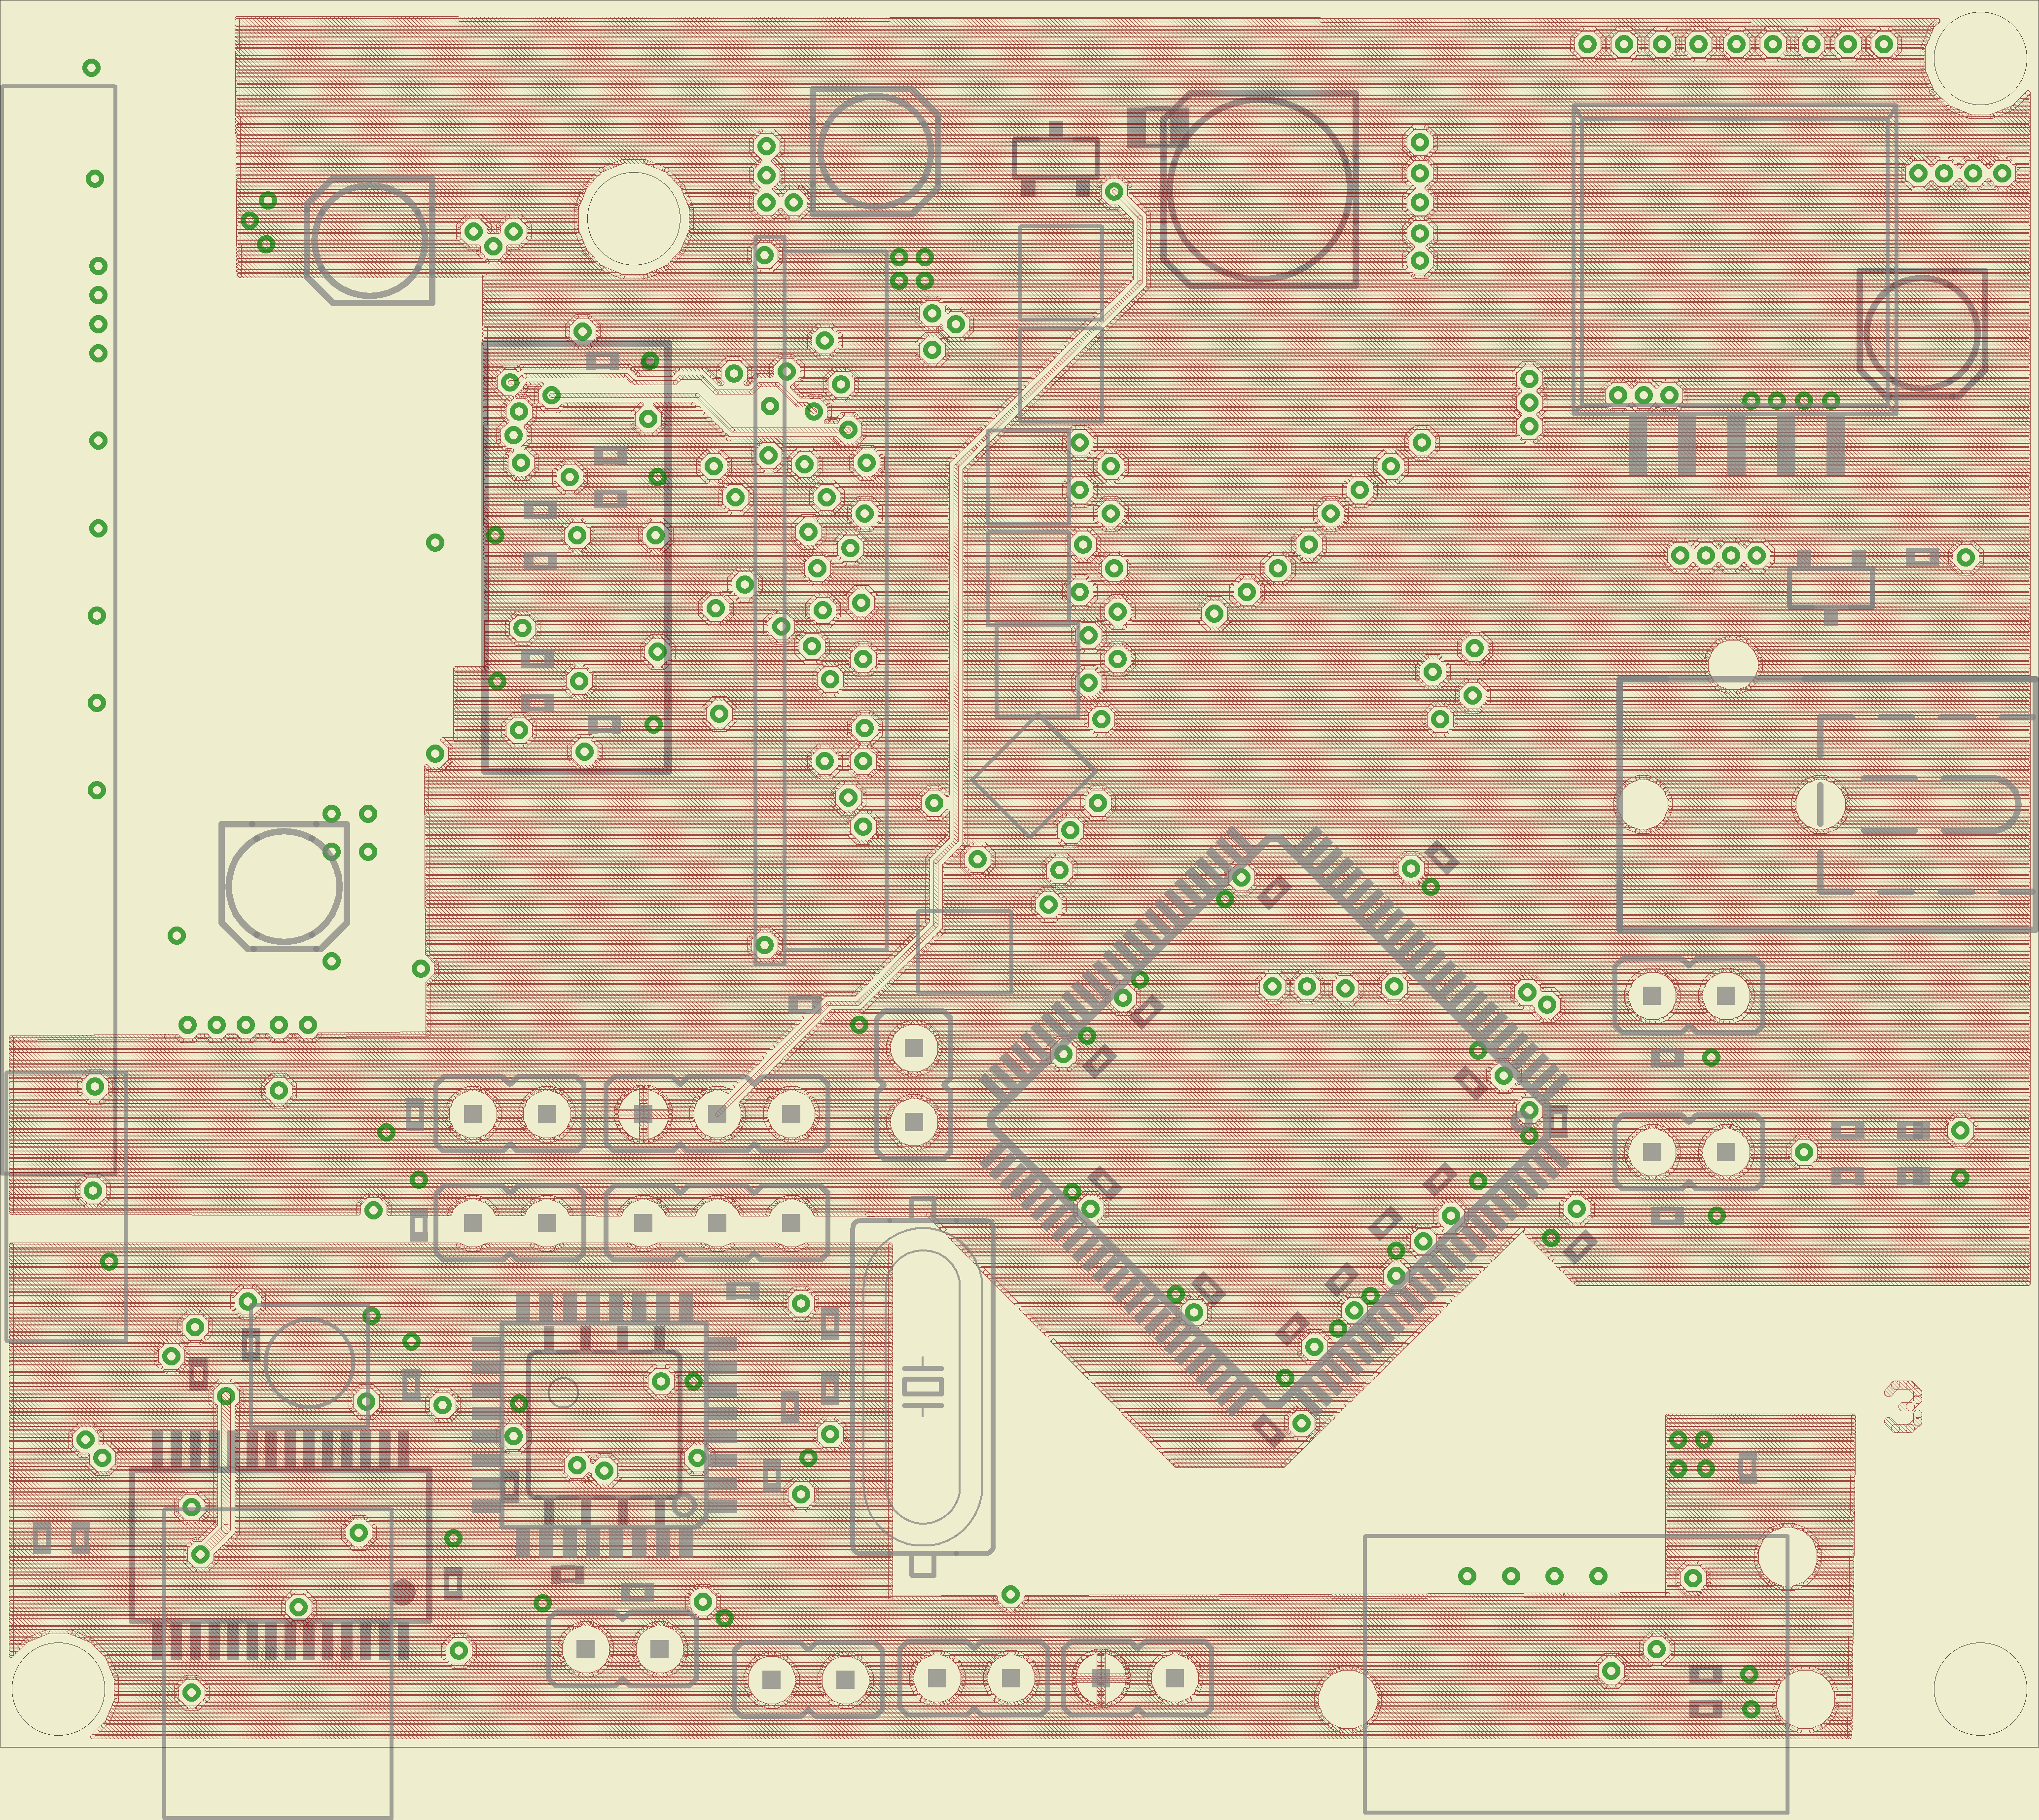
\includegraphics[width=1\textwidth]{TeilB/vcc_layer.png}}
                \caption{Versorgungs-Layer}
                \label{fig:teilb_vcc_layer}
        \end{subfigure}
		\quad 
        \begin{subfigure}[htp]{0.48\textwidth}
               \fbox{ 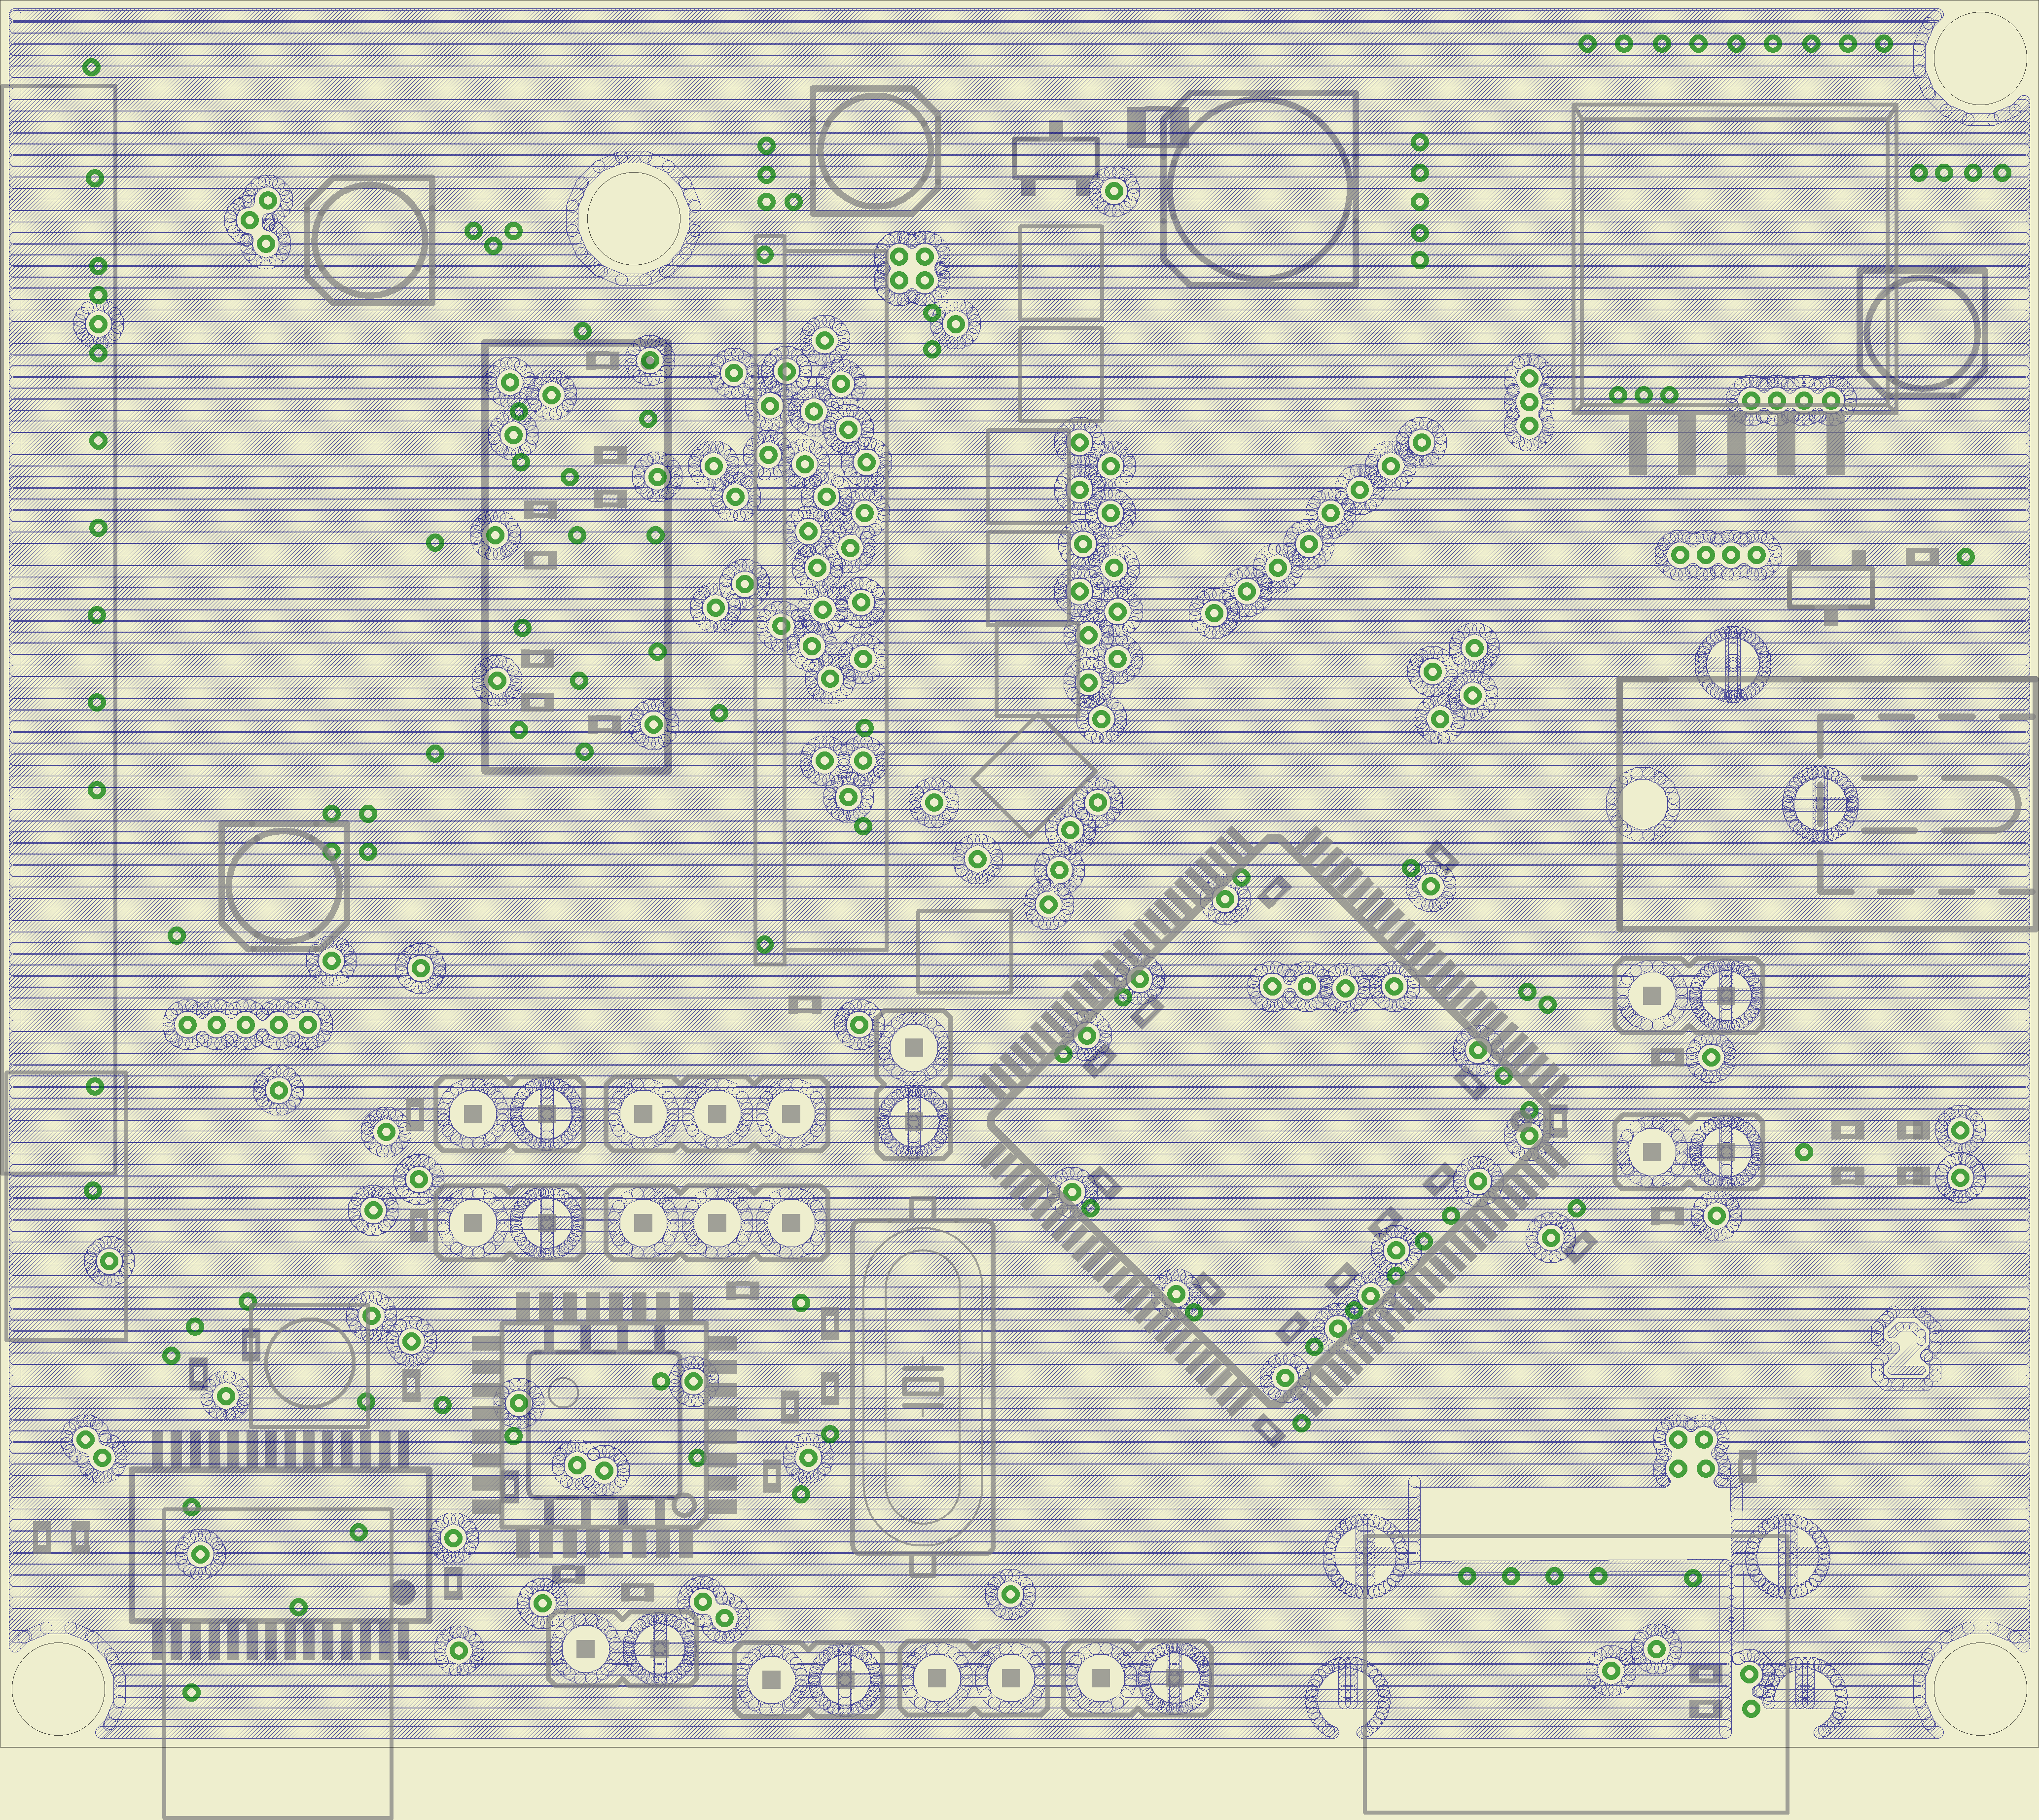
\includegraphics[width=1\textwidth]{TeilB/gnd_layer.png} }              								\caption{Ground-Layer}
                \label{fig:teilb_gnd_layer}
        \end{subfigure}
		%\end{center}
        \caption{Innenlagen}
        \label{fig:teilb_vcc_gnd_layer}
\end{figure}
Die obere Fläche in \refa{fig:teilb_vcc_layer} stellt die +3.3\,V-Versorgung dar. Die Bauteile sind durch kurze Wege mit Vias mit der Lage verbunden. Entsprechend ist die untere Fläche die +5\,V-Versorgung, vom HDMI-Stecker. Die Ground-Fläche ist in \refa{fig:teilb_gnd_layer} zu sehen. Sie umfasst fast die komplette Platine mit Ausnahme unter den Anschlüssen des HDMI-Steckers, da somit die Impedanz der HDMI-Leitungen besser angepasst werden (siehe \cite{TI2007}, S. 7). 